\documentclass[a4paper, 11pt, oneside]{report} 
\usepackage[utf8]{inputenc}
\usepackage[dutch]{babel}
\usepackage{diagbox}
\usepackage{amsmath}
\usepackage{amsfonts}
\usepackage{amssymb}
\usepackage{graphicx}
\usepackage{caption}
\usepackage[table,xcdraw]{xcolor}
\usepackage[toc,page]{appendix}
\usepackage{hyperref}
\usepackage{titlesec}
\usepackage{listings}
\usepackage{float}
\usepackage{tikz}
\usetikzlibrary{trees}
\usepackage{tikz-qtree}
\usepackage{graphicx}
\usepackage{fancyref}
\usepackage{wrapfig}
\usepackage{url}
\usepackage{pdflscape}
\usepackage{fancyvrb}
\usepackage{fancyhdr}
\graphicspath{ {Afbeeldingen/} }
\usepackage{subfig}
\usepackage{tabularx}
\usepackage{apacite}
\usepackage{longtable}
\usepackage{titlecaps}
%\usepackage[T1]{fontenc}
\usepackage{titlesec, blindtext, color}
\definecolor{gray75}{gray}{0.75}
\newcommand{\hsp}{\hspace{20pt}}
\usepackage{pdfpages}
\usepackage{booktabs}
\usepackage{listings}
\usepackage{siunitx}
\sisetup{per-mode=symbol,per-symbol = /,binary-units=true } 
\newcolumntype{L}[1]{>{\raggedright\arraybackslash}p{#1}}

\titleformat{\chapter}[hang]{\huge\bfseries}{\thechapter\hsp\textcolor{gray75}{|}\hsp}{0pt}{\Large\bfseries}

\makeatletter
\newcommand\tagreq[2]{#1\def\@currentlabel{#1}\label{#2}}
\makeatother

\def\checkmark{\tikz\fill[scale=0.4](0,.35) -- (.25,0) -- (1,.7) -- (.25,.15) -- cycle;} 
\def\figureautorefname{Figuur}
\def\subsectionautorefname{Subparagraaf}
\def\sectionautorefname{Paragraaf}
\def\chapterautorefname{Hoofdstuk}
\def\tableautorefname{Tabel}
\DeclareRobustCommand{\VAN}[3]{#2} % set up for citation

%% Sets page size and margins 
\usepackage[a4paper,top=3cm,bottom=3cm,left=3cm,right=3cm,marginparwidth=1.75cm]{geometry}

\definecolor{dkgreen}{rgb}{0,0.6,0}
\definecolor{gray}{rgb}{0.5,0.5,0.5}
\definecolor{mauve}{rgb}{0.58,0,0.82}



\lstset { %
	language=C++,
	backgroundcolor=\color{black!3}, % set backgroundcolor
	basicstyle=\footnotesize,% basic font setting
		numbers=none,
	numberstyle=\tiny\color{gray},
	keywordstyle=\color{blue},
	commentstyle=\color{dkgreen},
	stringstyle=\color{mauve},
	breaklines=true,
	breakatwhitespace=true,
	tabsize=3
}

\author{M.W.J. Berentsen}
\font\myfont=cmr12 at 40pt
\title{\myfont Drone meshnetwerk simulatie}
\usepackage{titling}

\newcommand{\subtitle}[9]{%
	\posttitle{%
		\par\end{center}
	\begin{center}\large#1\end{center}
	\begin{center}\large#2\end{center}
	\vskip0.5em
	\begin{center}\normalsize#3\end{center}
	\begin{center}\large#4\end{center}
	\begin{center}\large#5\end{center}
	\begin{center}\large#6\end{center}
	\begin{center}\normalsize#7\end{center}
	\begin{center}\normalsize#8\end{center}
	\begin{center}\normalsize#9\end{center}
	\vskip0.5em}%
	\rfoot{{\footnotesize \textbf{#1}}}
}

\subtitle{Onderzoeksrapport}{Versie 2.0}{Alten Nederland B.V.}{Hogeschool van Arnhem en Nijmegen}{HBO Technische Informatica - Embedded Software Developement }{MWJ.Berentsen@student.han.nl}{Studentnummer: 561399}{Docent: J. Visch, MSc}{Assessor: ir. C.G.R. van Uffelen}


\setlength{\parindent}{0pt}
\setlength{\parskip}{5pt plus 2pt minus 1pt}



\hypersetup{colorlinks=true, urlcolor=red,citecolor=black,linkcolor=blue}  % Colours hyperlinks in blue, but this can be distracting if there are many links.
\setcounter{tocdepth}{2}

\usepackage{fancyhdr}
\pagestyle{fancy}

\setlength\headheight{26pt} %% just to make warning go away. Adjust the value after looking into the warning.
% \rhead{{\color{blue}\rule{1cm}{1cm}}}

\rhead{
\includegraphics[height=1cm]{Afbeeldingen/han.png}}



\begin{document}
\begin{figure}
\begin{center}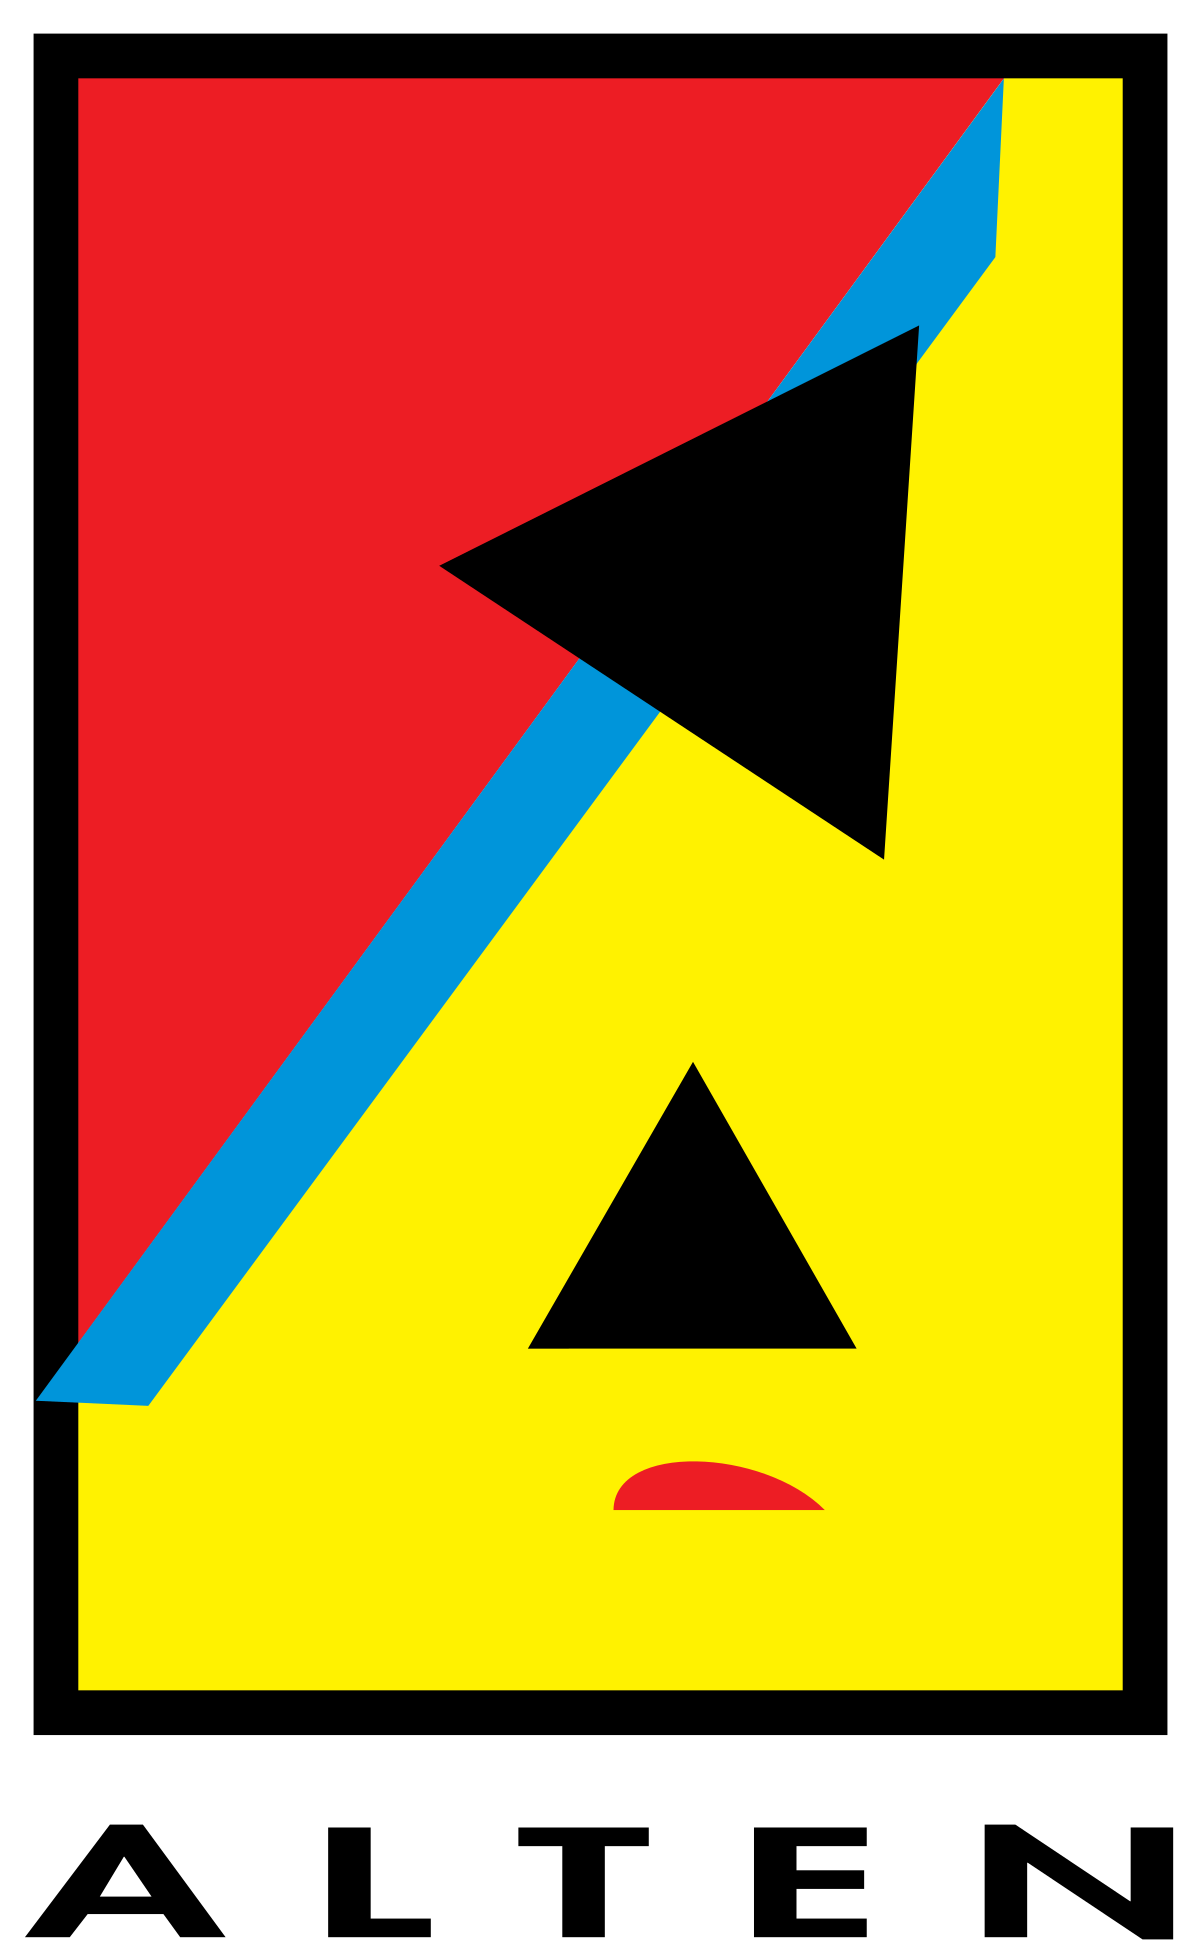
\includegraphics[scale=0.1]{alten}\end{center}
\end{figure}
\maketitle


\chapter*{Managementsamenvatting}

%\item Welke simulatiesoftware is geschikt om een netwerk van ongeveer 100 drones in na te bootsen?
%\item Wat is de grootte van de payload die een netwerkmodule aangesloten op een drone moet versturen om nuttig te zijn voor het aansturingssysteem?
%\item Welke meshnetwerk hardware is geschikt voor het onderling verbinden van drones?
%\item Welke meshnetwerk techniek is geschikt voor de te gebruiken hardware?
%\item Is het mogelijk voor een netwerkmodule om een netwerk te herstellen door het de mogelijkheid te geven zich vrij te bewegen?
%\item Wat is minimaal benodigd in een simulatie om abstracte drone te representeren?

In dit onderzoek word onderzocht hoe netwerkmodules een groep van honderd drones kunnen voorzien van een onderling meshnetwerk die snel kan reageren op uitval van netwerkpunten.

De drones moeten gesimuleerd worden. Onderzoek heeft aangetoond dat dit het beste gedaan kan worden in een combinatie van Ros met Gazebo.

Voordat er een onderzoek gestart kon worden naar welke antenne gebruik moest worden is er eerst gekeken hoe groot de berichten zijn die verstuurd worden.
Er is aangetoond dat een bericht die nuttig is voor het aansturingssysteem niet groter hoeft te zijn dan 16 bytes.

Literatuuronderzoek heeft aangetoond dat een nRF24l01+ antenne de meeste potentie heeft voor het meshnetwerk vanwege zijn snelheid van \SI{250}{\kilo\bit\per\second} op een afstand van 700 meter.

De gekozen controller om aan te sluiten op de drone is een Raspberry Pi model 2B+. Deze is gekozen door zijn compatibiliteit met een NRF24 en rijke I/O interface. 
De software voor het meshnetwerk is ontwikkeld voor het gebruik op een Raspberry Pi model 2B+ en geschreven in C++.   

Er is een aangepaste variant van het lightweight mobile routering protocol toegepast. Dit protocol gebruikt de flexibiliteit van het reactieve LMR protocol met een toevoeging van proactief gedrag wat het hybride maakt. De proactieve toevoeging zorgt ervoor dat de wens van Alten Nederland om snel achter uitval te komen uit komt. Daarnaast zorgt de toevoeging ervoor dat routes in het netwerk al bekend zijn voordat deze nodig zijn, wat zorgt voor snellere communicatie dan wanneer er op het moment dat het nodig is nog een pad gebouwd moet worden.

Om dit onderzoek te ondertussen is er een simulatie gebouwd waarin abstracte drones met daarop een aangesloten netwerkcomponent kunnen rondvliegen. Dit maakt de simulatie bruikbaar voor het testen van zowel routeringstechnieken als (her)verdelingen. 

Om aan te tonen dat de mogelijkheid om een drone te kunnen verplaatsen bijdraagt aan het zelfherstellend vermogen van een meshnetwerk is er een oplossing geïmplementeerd waar de drones een stap terug nemen in het netwerk, op het moment dat ze geen verbinding meer hebben.  Testen hebben aangetoond dat dit idee alleen een goede toevoeging is op het moment dat er een enkele drone uitvalt in een kritische verbinding. Op het moment dat er meer drones in een verbinding uitvallen komen de drones terug naar de gateway, waardoor er een potentieel groot deel van een netwerk wegvalt. Het doel om aan te tonen dat de simulatie bruikbaar is in het onderzoeken van (her)verdelingen is hiermee wel bewezen.

\tableofcontents
\clearpage


\chapter*{Begrippenlijst}
\label{inleiding:begrippenlijst}

\begin{longtable}[c]{|l|l|}
	\hline
	\rowcolor[HTML]{9B9B9B} 
	Term & Beschrijving \\ \hline
	\endhead
	%


	Byte & Een samenstelling van 8 bits. \\ \hline

	Debug & \begin{tabular}[c]{@{}l@{}}Term die slaat op debugger, vaak informatie die gebruikt \\ wordt om gedrag te vinden binnen een applicatie.\end{tabular} \\ \hline
	Gateway & Een toegangspunt tot een netwerk. \\ \hline
	Gazebo & Simulatiesoftware met ondersteuning voor physics. \\ \hline
	GPS & Systeem voor locatie en tijd bepaling. \\ \hline


	nRF24l01+ & Radio transciever module werkzaam op de 2,4Ghz band. \\ \hline
	Physics engine & Software die natuurwetten toepast op virtuele objecten. \\ \hline
	\begin{tabular}[c]{@{}l@{}}Raspeberry Pi \\ model 2B+\end{tabular} & Micro computer geschikt voor prototyping. \\ \hline
	Ros & \begin{tabular}[c]{@{}l@{}}Robot operating system. Wordt gebruikt voor de transportlaag \\ naar zowel virtuele als gesimuleerde robots.\end{tabular} \\ \hline


	Router & Netwerkcomponent die berichten kan doorsturen. \\ \hline
	Routeringstechniek & \begin{tabular}[c]{@{}l@{}}Techniek die gebruikt voor het opbouwen van een pad binnen\\ een netwerk.\end{tabular} \\ \hline


	Seriële verbinding & Een communicatieverbinding het meest bekend van USB. \\ \hline
	Simulatie software & Software die fysieke objecten nabootst in software. \\ \hline

	\caption{Begrippenlijst.}
	\label{tab:begrippenlijst}\\
\end{longtable}%\label{begrippen}




\chapter{Inleiding}
\label{chapter:inleiding}


Het volgende onderzoeksrapport wordt uitgevoerd ten behoeve van het afstudeerproject van Maurice Berentsen, Hogeschool van Arnhem en Nijmegen.

Het doel van dit onderzoek is het zetten van de eerste stap in de ontwikkeling van het dronenetwerk.
De eerste stap is het ontwikkelen van een simulatie van een netwerkmodule voor het onderling verbinden van drones.
Het is van belang dat het meshnetwerk van de drones snel kan reageren op uitval van netwerkpunten en dat er eerst uitgezocht wordt welke hardware de netwerkmodule moet gebruiken.

De aanleiding om dit onderzoek uit te voeren is om de kennis te verschaffen die nodig is om een netwerk van drones te kunnen opzetten.
Door het ontwikkelen van een simulatie die gebaseerd is op keuzes voor de werkelijke drones en netwerkapparatuur kunnen er tijdens dit onderzoek al testen worden uitgevoerd zonder dat er de benodigde hardware zoals drones, antennes en microcomputers aanwezig hoeven zijn. 


\chapter{Hoofd- en deelvragen}
In dit hoofdstuk worden de hoofd- en deelvragen genoemd en onderbouwd.
Er wordt een scope bepaalt met wat er onderzocht wordt en dus ook wat niet.
Vervolgens wordt de onderzoeksmethode toegelicht en beargumenteerd.
Tenslotte wordt de invloed van het onderzoek op het afstudeerproject beschreven.

\section{Hoofdvraag}
Het doel van dit onderzoeksrapport is het beantwoorden van de volgende opgesteld hoofdvraag:
\begin{quotation}
\textit{``Hoe kunnen netwerkmodules een groep van ongeveer 100 drones voorzien van een onderling meshnetwerk die snel reageert op uitval van netwerkpunten?''}	
\end{quotation}
Doordat de uitvoerende student van dit onderzoek niet beschikt over een certificaat om met drones te mogen vliegen behoudt dit onderzoek zich tot een simulatie.


\section{Deelvragen}

Om de hoofdvraag te kunnen beantwoorden zijn er de volgende deelvragen opgesteld:

\begin{itemize}
	\item Welke simulatiesoftware is geschikt om een netwerk van ongeveer 100 drones in na te bootsen?
	\item Wat is de grootte van de payload die een netwerkmodule aangesloten op een drone moet versturen om nuttig te zijn voor het aansturingssysteem?
	\item Welke meshnetwerk hardware is geschikt voor het onderling verbinden van drones?
	\item Welke meshnetwerk techniek is geschikt voor de te gebruiken hardware?
	\item Is het mogelijk voor een netwerkmodule om een netwerk te herstellen door het de mogelijkheid te geven zich vrij te bewegen?
	\item Wat is minimaal benodigd in een simulatie om abstracte drone te representeren?
\end{itemize}

\section{Onderzoeksmethode}
De onderzoeksmethodes volgen de structuur van de \textit{ICA methodenkaart} \cite{MethodenKaart}.
De methodenkaart is een onderzoek framework voor professionals in ICT en media.
Het ontwerp van het framework gaat uit van het idee van triangulatie.
Triangulatie is het combineren van verschillende theorieën, methoden of databronnen om zo tot betere antwoorden te komen op je onderzoeksvragen \cite{ICAoates}. 
Door het definiëren van zo geheten werkplaatsen en hun samenhang geeft het de onderzoeker een set van methoden en technieken. 
De vijf verschillende werkplaatsen binnen het framework zijn: \textit{lab, veld, showroom, bieb en werkplaats}.

\begin{figure}[H]
	\begin{center}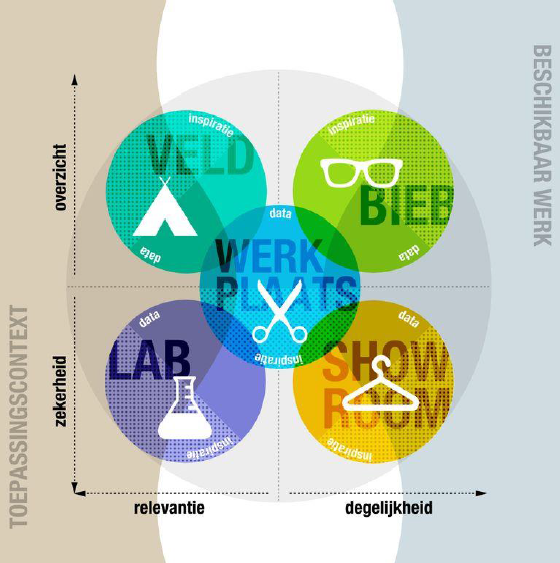
\includegraphics[width=0.5\linewidth]{Methodenkaart}\end{center}
	\caption{De vijf werkplaatsen binnen het framework en hun systematiek. Overgenomen uit \textit{De informatieprofessional 3.0}  van \protect\citeA{MethodenKaart}.}
	\label{fig:methodenkaart}
\end{figure}

\subsection{De gekozen onderzoeksmethodes}

De deelvragen gaan gedeeltelijk over keuzes van gebruik. 
Welke software en hardware is geschikt, is een vraag die veel naar voren komt.
Hieruit valt te concluderen dat de onderzoeker zich nog aan het oriënteren is.
``De onderzoeksruimte bieb bevat een verzameling methoden en technieken die dienen tot oriëntatie op beschikbaar werk."\cite{MethodenKaart}.
Daarom wordt er gekozen om een bieb onderzoek uit te voren naar de deelvragen die gaan over geschiktheid.
Dit zodat de onderzoeker zich nog kan oriënteren naar het beschikbare aanbod en op nieuwe deelvragen kan komen. 

Lab onderzoek wordt pas later uitgevoerd omdat niet alle hardware voor handen is, maar ook omdat er niet genoeg tijd voor beschikbaar is.
\citeauthor{MethodenKaart} zegt het volgende over lab onderzoek: De onderzoeksruimte lab bevat methoden die geschikt zijn om de oplossing te toetsen aan een aspect van de toepassingscontext.
Daarom is het lab onderzoek geschikt voor het moment waarop de hardware beschikbaar is en de onderzoeker het gedrag hiervan exact in kaart wil brengen en wil bewijzen dat de gestelde eisen behaald worden.

\citeA{ICAoates} stelt dat een systeem bouwen 'bewijs' is dat een nieuw soort toepassing gebouwd kan worden. Als dit het doel is heeft het onderzoek waarschijnlijk hoofdzakelijk een werkplaats karakter, maar alle andere onderzoeksruimtes kunnen een rol spelen.
Gedurende het huidige onderzoek zal er door de onderzoeker software geschreven worden om bewijs te leveren dat een netwerkmodule een groep drones kan voorzien van een onderling netwerk.
Daarom past de werkplaats onderzoeksruimte goed bij dit onderzoek.


\section{Invloed op het project}

Het onderzoek is van invloed op het project waarin de opdracht is om een simulatie van drones voorzien van een netwerkmodule te bouwen.
De kennis die uit dit onderzoek wordt gehaald beïnvloed de keuzes in het gebruik van zowel hardware als software. 
Zo zal er gekeken worden hoe groot een bericht mag zijn wat van invloed is op de software die berichten gebruikt.
Er wordt onderzoek gedaan welke antenne geschikt is voor het project wat de hardwarekeuze beïnvloed.
Tenslotte wordt er ook onderzocht welke simulatiesoftware gebruikt moet worden wat van grote invloed is op het project.

Daarnaast worden er in dit onderzoek ook oplossingsrichtingen bedacht die geïmplementeerd en getest zullen worden in de gebouwde software. 

\chapter{Criteria}
\label{chapter:criteria}

In \autoref{tab:criteria} worden codes gebruikt als naam voor de criteria, wat deze betekenen wordt eerst toegelicht:
\begin{itemize}
	\item ALG: Een algemene eis die in elke onderzoek meegenomen moet worden.
	\item SK: Een eis die gesteld worden in de keuze naar simulatiesoftware.
	\item DR: Een eis voor de te gebruiken drone in de simulatie.
	\item PH: Eisen opgesteld aan de prototype hardware.
	\item PS: Eisen opgesteld aan de prototype software.
\end{itemize}

\begin{longtable}{|l|l|l|}
	\hline
	\rowcolor[HTML]{C0C0C0} 
	Naam & Beschrijving \\ \hline
	%\endfirsthead
	%
	\endhead
		\hypertarget{alg1}{ALG1}	&Is voorzien van API documentatie.        \\ \hline
		\hypertarget{alg2}{ALG2}	&Ondersteunt aansturing vanuit C++.    \\ \hline
		\hypertarget{alg3}{ALG3}	&\begin{tabular}[c]{@{}l@{}}Heeft ondersteuning voor het Linux platform Ubuntu 18.04.\end{tabular}        \\ \hline
		\hypertarget{alg4}{ALG4}	&Software is gratis in gebruik voor studenten.        \\ \hline
		\hypertarget{sk1}{SK1}		&\begin{tabular}[c]{@{}l@{}}Heeft ondersteuning voor UAV's (unmanned air vehicle) ook wel drones genoemd.\end{tabular} \\ \hline
		\hypertarget{sk2}{SK2}		&\begin{tabular}[c]{@{}l@{}}Ondersteunt de simulatie van locatiebepaling sensoren zoals GPS.\end{tabular}        \\ \hline
		\hypertarget{sk3}{SK3}		&\begin{tabular}[c]{@{}l@{}}Heeft een kant en klare oplossing voor simulatie van externe krachten zoals wind.\end{tabular}        \\ \hline
		\hypertarget{sk4}{SK4}		& Heeft een ingebouwde pathfinding oplossing.        \\ \hline
		\hypertarget{sk5}{SK5}		& Ondersteunt Ros als middleware.        \\ \hline
		\hypertarget{sk6}{SK6}		& Ondersteunt de detectie van botsingen.        \\ \hline
		\hypertarget{sk7}{SK7}		& Ondersteunt de simulatie 100 drones tegelijk.        \\ \hline
		DR1		& De drone is een quadcopter.        \\ \hline
		DR2		& De drone is is voorzien van een API voor aansturing op basis van coördinaten.       \\ \hline
		DR3		& De API sluit aan op de middleware Ros melodic.        \\ \hline
		DR4		& De drone is bruikbaar binnen de gekozen simulatiesoftware Gazebo.        \\ \hline
		DR5		& De drone moet een kleine goedkope drone representeren.        \\ \hline
		\hypertarget{ph1}{PH1}		& Ondersteunt een bereik van minimaal 500 meter.  \\ \hline
		\hypertarget{ph2}{PH2}		& Ondersteunt het gebruik van grid networking om tot een mesh te kunnen komen.  \\ \hline
		\hypertarget{ph3}{PH3}		& Maakt gebruik van een openbare bandbreedte.\\ \hline
		\hypertarget{ph4}{PH4}		& Voorziet zichzelf van een draadloos netwerk en leunt dus niet op technieken zoals 4G.\\ \hline
		\hypertarget{ph5}{PH5}		& Is een product ontwikkeld voor low energy toepassingen. \\ \hline
		PS1		& Ondersteunt een meshnetwerk van minimaal 100 nodes. \\ \hline
		PS2		& Het netwerk is zelf herstellend. \\ \hline
		PS3		& Ondersteunt het draaien op een Raspberry Pi model 2B+ \\ \hline
		PS4		& Ondersteunt het versturen van zelfgemaakte berichten. \\ \hline
		
	\caption{Opgestelde criteria.}
	\label{tab:criteria}
\end{longtable}

\chapter{Literatuur}


\section[Welke simulatiesoftware?]{Welke simulatiesoftware is geschikt om een drone in na te bootsen?}
\label{sec:welkesim}
Voor het onderzoek wordt gebruik gemaakt van een simulatieomgeving.
Welke software gebruikt moet worden staat vastgesteld in deze paragraaf.
De keuze van software wordt bepaald door het uitvoeren van de bieb onderzoeksmethode. 
In de \autoref{tab:criteria} staan de criteria toegelicht waar de simulatiesoftware aan moet voldoen.
Als hoofdcriteria wordt een lijst opgesteld met simulatoren, die ondersteuning hebben voor Ros.
Vervolgens worden deze aan de hand van een kruistabel onderworpen aan de andere criteria.
Deze techniek is gebaseerd op de "Comparison Chart" van \cite{CMDmethod} uit de "\textit{CMD Methods Pack}"

De kandidaten zijn:
\begin{itemize}
	\item Actin is een simulatie framework van het bedrijf Energid. Het is in staat om de beweging van verschillende robots gelijktijdig aan te sturen \cite{energid}.
	
	\item Gazebo is een open source robot simulatie framework bijzonder geschikt voor het simuleren van robotica in outdoor-omgevingen door de uitgebreide Physics Engine Support \cite{gazebo}.
	\item V-REP (Virtual Robot Experimentation Platform) is een platform geschikt voor het snel bouwen van robot prototypes \cite{vrep}.
	\item Webots is een open source ontwikkelomgeving die wordt gebruikt voor het modelleren, programmeren en simuleren van mobiele robots \cite{webots}.
	\item OpenRAVE biedt een ontwikkelomgeving voor het testen van motion planning algoritmes aan de hand van simulaties \cite{openrave}.
\end{itemize}

\begin{table}[H]
	\centering
	\begin{tabular}{l|*{10}r}
		%\backslashbox{Input}{Output} & int8\_t & int16\_t & int32\_t & uint8\_t & uint16\_t & uint32\_t \\
		\diagbox[width=2.7cm, height=2.4cm]{\raisebox{5pt}{\hspace*{0.25cm}Simulator}}{\raisebox{-1.27cm}{\rotatebox{90}{Eis}}} & \raisebox{-0.25cm}{\rotatebox{90}{\hyperlink{alg1}{ALG1}}} & \raisebox{-0.25cm}{\rotatebox{90}{\hyperlink{alg2}{ALG2}}} & \raisebox{-0.25cm}{\rotatebox{90}{\hyperlink{alg3}{ALG3}}} & \raisebox{-0.25cm}{\rotatebox{90}{\hyperlink{alg4}{ALG4}}} &
		\raisebox{-0.25cm}{\rotatebox{90}{\hyperlink{sk1}{SK1}}} & \raisebox{-0.25cm}{\rotatebox{90}{\hyperlink{sk2}{SK2}}} &
		\raisebox{-0.25cm}{\rotatebox{90}{\hyperlink{sk3}{SK3}}} & \raisebox{-0.25cm}{\rotatebox{90}{\hyperlink{sk4}{SK4}}} &
		\raisebox{-0.25cm}{\rotatebox{90}{\hyperlink{sk5}{SK5}}} & \raisebox{-0.25cm}{\rotatebox{90}{\hyperlink{sk6}{SK6}}} \\
		\midrule\\
		\hspace*{0.25cm}Actin 	& \checkmark & \checkmark 	& \checkmark & x 		  & \checkmark & x 			& \checkmark & x 		  &\checkmark & \checkmark	\\ \\
		\hspace*{0.25cm}Gazebo 	& \checkmark & \checkmark 	& \checkmark & \checkmark & \checkmark & \checkmark & \checkmark & \checkmark &\checkmark & \checkmark	\\ \\
		\hspace*{0.25cm}V-REP 	& \checkmark & x 			& \checkmark & \checkmark & \checkmark & \checkmark & \checkmark & \checkmark &\checkmark & x	\\ \\
		\hspace*{0.25cm}Webots 	& \checkmark & \checkmark 	& \checkmark & \checkmark & \checkmark & \checkmark & \checkmark & \checkmark &\checkmark & \checkmark 	\\ \\
		\hspace*{0.25cm}OpenRAVE& \checkmark & \checkmark	& \checkmark & \checkmark & x 		   & \checkmark & \checkmark & \checkmark &\checkmark & x 	\\ \\
		\bottomrule
	\end{tabular}%
	\caption{Kruistabel simulatiekeuze.}
	\label{tab:kruissimkeuze}%
\end{table}%

In de \autoref{tab:kruissimkeuze} komt de simulatiesoftware van Gazebo en Webots naar voren als enige simulatoren die voldoen aan alle gestelde eisen.
Het is nu zaak om te uit te zoeken welke van de twee het meest geschikt is voor het uitvoeren van dit onderzoek.

\subsection{Gazebo of Webots?}
In januari 2018 hebben \citeauthor{RobotCompare} een publicatie geschreven waarin zij drie simulatoren vergelijken in het aanbod van features en performance \cite{RobotCompare}. 
Zij hebben een vergelijking gedaan tussen V-REP, Gazebo en ARGoS. 
ARGoS is niet meegenomen in de overweging voor het huidige onderzoek omdat het geen ondersteuning heeft voor Ros.

Uit de resultaten van de publicatie blijkt dat Webots als het meest gebruiksvriendelijk naar voren in het gebruik en is in het bezit van de meeste features.
Het grote nadeel van Webots is dat het veel kracht vraagt van de computer, waardoor het niet geschikt is voor de simulatie van meerdere drones tegelijk.

Daarmee komt de keuze uit op Gazebo. 
De resultaten in de publicatie van \citeA{RobotCompare} tonen aan dat de software in staat is om veel drones tegelijk aan te kunnen sturen.
\citeA{RobotCompare} geven als nadeel aan Gazebo dat de software niet in staat is om 3d meshes te manipuleren, de user interface niet innovatief is en Gazebo soms problemen heeft met dependencies door de verschillende versies van Ros.
Dit laatste brengt een risico met zich mee voor het onderzoek daarom is het ook zaak dat dit als criteria meegenomen word in de deelvraag van \autoref{sec:dronekeuze} \nameref{sec:dronekeuze}. 

\subsection{Conclusie}
Voor het onderzoek wordt Gazebo gebruikt omdat het voldoet aan de gestelde \nameref{chapter:criteria}.
De meest recente stabiele versie van Gazebo is Gazebo 9.
Deze versie vereist het gebruik van Ros Melodic volgens haar eigen website \cite{versiongazeb}.

\section[Welke grootte voor de payload?]{Wat is de grootte van de payload die een netwerkmodule aangesloten op een drone moet versturen om nuttig te zijn voor het aansturingssysteem?}

De payload is het gedeelte van een bericht die vrij is naar de gebruiker om invulling te geven.
De maximale grote van een payload verschilt per protocol.
Om een keuze te kunnen maken waar de hardware en het bijhorende protocol aan moet voldoen is het dus zaak om eerst te weten hoe groot deze vrije payload ruimte moet zijn.

Het doel van de berichten is om ze zo kort als mogelijk samen te stellen. 
Daarom is het belangrijk om de structuur van de berichten zo klein mogelijk te houden.
Om deze reden wordt niet gekeken naar een tekstuele serialisatie mogelijkheden zoals XML, YAML, JSON maar naar binaire mogelijkheden, omdat deze veel efficienter zijn \cite{binary}.

\subsection{Binaire serialisatie voor het samenstellen van berichten} 

"Binary Serialization is converting the object in binary format and being able to store it in a storage medium"\cite{binary}. 
Het binair samenstellen van informatie is een efficiënte manier, omdat de data met een minimale overhead wordt samengesteld \cite{binaryMessaging}.
Het nadeel die deze wijze met zich meebrengt is dat het resultaat van het bericht niet meer makkelijk leesbaar is voor mensen.
Tijdens dit project ligt daar geen focus op, dus is dit nadeel te verwaarlozen.

\citeA{binaryMessaging} hebben onderzoek gedaan naar een efficiënte manier van de inzet van binaire berichten ter vervanging van tekstuele serialisatie.
Hoewel dat in het huidige onderzoek niet het geval is, kan er wel geleerd worden hoe de berichten gebruikt worden.
\citeA{binaryMessaging} tonen in hun onderzoek aan dat berichten vaak een herhalende structuur hebben en dat dit een onnodige overhead creëert in de berichten.
Een voorbeeld maken \citeA{binaryMessaging} zichtbaar in \autoref{fig:jsonxml} waarover zij het volgende zeggen: "While JSON  compared  with  XML,  eliminated  parameter  name redundancy, it keeps repeating (red box) the definition of each field  for  each  serialized  element  (green  box)". 
\begin{figure}[H]
	\begin{center}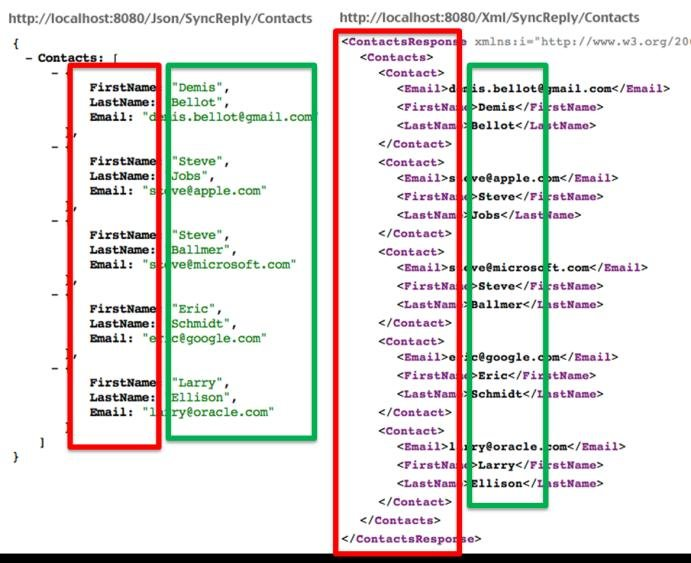
\includegraphics[width=0.5\linewidth]{JSONandXML.jpeg}\end{center}
	\caption{JSON and XML messages. Overgenomen uit \textit{International Journal of Computer Applications}  van \protect\citeA{binaryMessaging}.}
	\label{fig:jsonxml}
\end{figure}

Wat zij hebben gedaan om dit op te lossen is het apart versturen van de parameternamen zodat deze in de opvolgende berichten van dat type niet meer nodig is.
Het systeem die bedacht is geeft een enorme flexibiliteit omdat er van te voren nog geen bericht types bekend hoeven te zijn.
Deze flexibiliteit is alleen niet van toepassing op het doel van dit project, daarom kan de student in zijn software al van te voren berichttypes samenstellen waardoor de overhead nog kleiner gemaakt wordt.
Voor nu wordt er vanuit gegaan dat 1 byte genoeg zal zijn omdat de communicatiesoftware van de netwerkmodule niet meer dan 256 ($2^{8}$) berichtentypes hoeft te ondersteunen.
Mocht het blijken dat dit toch niet genoeg is kan er er een byte toegevoegd worden waardoor er 65536 ($2^{16}$) types mogelijk zouden zijn.
Daarnaast moet een bericht om nuttig te zijn voor het netwerk altijd aan een apparaat gekoppeld kunnen worden.
De opdracht gaat over een netwerk van ongeveer 100 drones wat ruim past in een byte.
Daarom wordt er gekozen om een byte te gebruiken wat 255 unieke ID's mogelijk zou maken. 
Hiermee komt het eerste deel van het bericht dus al tot stand het telt nu minimaal 2 bytes.

\begin{table}[H]
	\centering
	\begin{tabular}{|l|l|l|}
		\hline
		\rowcolor[HTML]{C0C0C0} 
		ID & Berichttype & overig \\ \hline
		00 tot FF   & 00 tot FF       & ?      \\ \hline
	\end{tabular}
	\caption{Berichtsamenstelling met type aanduiding.}
	\label{tab:serialstart}
\end{table}

\subsection{Wat is nuttige informatie die in een bericht kan staan voor of van een aansturingssysteem?}
\label{sub:watisnuttigeinformatie}
Het is nog niet bekend is welk type netwerk er gebruikt gaat worden.
Wat al wel bekend is dat dit een low power long range netwerk zal zijn om aan de requirements te voldoen.
Een gedeelde eigenschap van zulke netwerken is de lage bandbreedte waardoor ze niet geschikt zijn voor realtime applicaties.
Deze kennis kan toegepast worden op de informatie die de drones met hun netwerkmodules bij zich dragen. 
Informatie zoals snelheid en richting heeft geen prioriteit om verstuurd te worden omdat deze niet relevant is voor het aansturingssysteem aangezien hier geen beslissingen op gebaseerd kunnen worden.
Wat wel van belang is voor het aansturingssysteem is informatie als waar bevindt een netwerkmodule zich op welk moment in tijd.
Daarnaast kan informatie zoals de status van de batterij en de sterkte van de verbinding van belang zijn voor het systeem omdat deze informatie gebruikt kan worden om preventieve beslissingen te nemen in het onderhoud van het netwerk.

Een bericht die het aansturingssysteem tenminste zal verzenden zal het commando zijn om een drone naar een coordinaat te sturen.
Daarnaast zal er een bericht moeten komen waarmee het systeem de status van het netwerk kan controleren, wat voor bericht dit zal zijn is nog niet bekend.


\subsection{Wat is de grootte van een bericht voor de locatie bepaling van drones?}
\label{sub:locatie}
De huidige locatie is essentiële administratie voor de verdeling van de drones.
Omdat de drones zich kunnen verplaatsen is naast de locatie ook het tijdstip waarop het bericht verstuurd wordt van belang.

\subsubsection{Coördinaat vanuit de informatie van de GPS module}
Een positie van een locatie wordt aangeduid door coördinaten te gebruiken.
Deze worden bepaald door het gebruik van een GPS module aan boord van het systeem.
GPS modules gebruiken triangulatie van satellietsignalen om hun positie te bepalen.  

Een coördinaat is opgebouwd door de aarde te verdelen in graden over de assen latitude (horizontaal) en longitude (verticaal).
Een coördinaat loopt van -180 tot 180 graden.
De aarde heeft een omtrek van 40.07.5161,2 meter gedeeld door 360 graden levert dit per graad een stap op van 111,32 kilometer. 
Het volgende programma laat zien dat een float gebruikt kan worden in dit geval voor een accuraatheid van 5 cijfers achter het decimaal.

\begin{lstlisting}
#include <stdio.h>

float exampleFloatPositive = 179.1234567890;
float exampleFloatNegative = -179.1234567890;

int main( int argc, const char* argv[] )
{
	printf( "postive  float =  %f\n", exampleFloatPositive );
	printf( "negative float =  %f\n", exampleFloatNegative );
}
\end{lstlisting}
 
Door een coördinaat te gebruiken van 5 cijfers achter het decimaal kan een plek op aarde met een precisie van ongeveer 1,10 meter nauwkeurig aangeven worden.
Het is gebruik hiervan is realistisch omdat met alleen realtime GPS data de accuraatheid ongeveer 4 meter is \cite{GPSaccu}.
Er wordt per as een float gebruikt dit houdt in dat minimaal 8 bytes nodig zijn voor een coördinaat.
Dit zijn 4 bytes per float exclusief de separator. 

\subsubsection{Hoogte van de drone}
\citeA{GPSheight} hebben onderzoek gedaan naar de accuraatheid van de hoogtebepaling bij drones. 
Uit dit onderzoek is gebleken dat een continue vliegende drone een hoogte accuraatheid heeft van ongeveer twee meter.
Hieruit is te halen dat het geen zin heeft om op 'centimeter niveau' de hoogte van een drone aan te geven.
Op het moment dat er een signed integer van 16 bits gebruikt zou worden kan er een afstand van 32.767 meter zowel boven als onder zeeniveau verstuurd worden.
Het is een realistische waarde om te gebruiken, aangezien de grootste hoogte die gebruik kan worden dan 32 kilometer is.
Deze hoogte is al ver in de stratosfeer en zelfs al boven het niveau die een weerballon haalt. 
De keuze om een signed integer te gebruiken is om ondersteuning te bieden aan plekken onder het zeeniveau waarvan Nederland een goed voorbeeld is.

Voor de hoogte moeten 2 bytes gereserveerd worden. 

\subsubsection{Tijd vanuit de GPS module}

De drone maakt al gebruik van de GPS module voor de positiebepaling.
In de berichten die de GPS module ontvangt van de satellieten wordt ook de tijd meegestuurd.
Deze tijd is volgens \cite{GPSaccu} in 95 procent van de gevallen accuraat tot 40 Nano seconden. 
In het geval van het drone netwerk is dit veilig te gebruiken als bron voor tijd.
De tijd zal aangegeven worden in het unix time format zodat deze meteen de datum met zich draagt.
Unix time maakt gebruik van 32 bits formaat, er is gekozen voor een unsigned variant aangezien er geen interesse is naar data voor 1 januari 1970 ook wel epoch genoemd.

Voor de tijd en datum worden 4 bytes gereserveerd.

\subsubsection{Conclusie}  

De bovenstaande sub paragrafen kunnen samengesteld worden tot een bericht waarin alle informatie zit die nodig is om te bepalen waar een drone zich op een moment bevindt.
Een systeem kan met dit bericht in ieder geval elke drone afzonderlijk in kaart brengen.

\begin{table}[H]
	\centering
\begin{tabular}{l|l|l|l|l|l|l|}
	\cline{2-7}
	& \cellcolor[HTML]{C0C0C0}ID & \cellcolor[HTML]{C0C0C0}\begin{tabular}[c]{@{}l@{}}Bericht \\ type\end{tabular} & \cellcolor[HTML]{C0C0C0}latitude & \cellcolor[HTML]{C0C0C0}longitude & \cellcolor[HTML]{C0C0C0}hoogte & \cellcolor[HTML]{C0C0C0}tijd \\ \hline
	\multicolumn{1}{|l|}{\cellcolor[HTML]{C0C0C0}\begin{tabular}[c]{@{}l@{}}Aantal\\ Bytes\end{tabular}} & 1                          & 1                                                                               & 4                                & 4                                 & 2                              & 4                            \\ \hline
\end{tabular}
 \caption{Locatie bericht in bytes.}
\label{tab:locatiebericht} 
\end{table}
In \ref{tab:locatiebericht} is het aantal bytes te zien benodigd voor een locatie bericht.
Als conclusie is bepaald dat voor dit bericht een grootte van minimaal 16 bytes gebruikt.
 
\subsection{Wat is de grootte van een bericht waarin een netwerkmodule zijn verbinding met anderen aangeeft?}

Eén van de wensen van de Alten is het in kaart brengen van de onderlinge verbindingen van de modules in het drone netwerk. 
Als voorbeeld hoe dit eruit kan zien is de schets afkomstig van de casus uit het plan van aanpak toegevoegd als bijlage te vinden in \autoref{app:schetsNetwerk}.
De informatie van de locatie van de netwerkpunten zijn al bekend door het gebruik van het bericht in \autoref{sub:locatie}.
Wat overblijft als onbekende informatie is de onderlinge verbinding.

In het netwerk kunnen twee rollen verdeeld worden.
\begin{itemize}
\item De rol van zender aan het device die informatie wil versturen naar het basis station.
\item De rol van ontvanger aan het device die de informatie van zender ontvangt.
\end{itemize}
Een device die beide rollen kan aannemen wordt een transceiver genoemd.
Als werkbaar voorbeeld wordt het netwerk uit de \nameref{app:schetsNetwerk} gebruikt.
De ontvangers en zenders zijn verdeelt in \autoref{tab:ontvangerzender}.

\begin{table}[H]
\centering
\begin{tabular}{
		>{\columncolor[HTML]{C0C0C0}}r |c|c|c|c|c|c|c|c|c|c|c|c}
	Ontvanger & BS   & 9   & 7 & 5 & 3 & 2 & 8 & 6 & 11    & 13 & 12 & 14       \\ \hline
	Zender    & 9,11 & 7,8 & 5 & 3 & 2 & 1 & 6 & 4 & 13,10 & 12 & 14 & 15,16,17
\end{tabular}
	\caption{De ontvangers en zenders uit de casus.}
	\label{tab:ontvangerzender}
\end{table} 

\subsubsection{Topologie met PlantUML}  
Om snel aan te kunnen tonen dat er weinig informatie nodig is om een topologie op te stellen gebruikt de student PlantUML.
Hiermee wordt aangetoond dat een bericht die de ontvanger aanmaakt zodra een zender zich bij hem aanmeld waar in staat wie de zender is genoeg is voor een topologie.
De keuze om de verantwoording bij de ontvanger neer te leggen is omdat een zender niet bij elke soort netwerk weet wie de ontvanger is.
De uitwerking hiervan is zichtbaar in \autoref{fig:toplogienetwerkuml}.

\begin{figure}[H]
	\begin{center}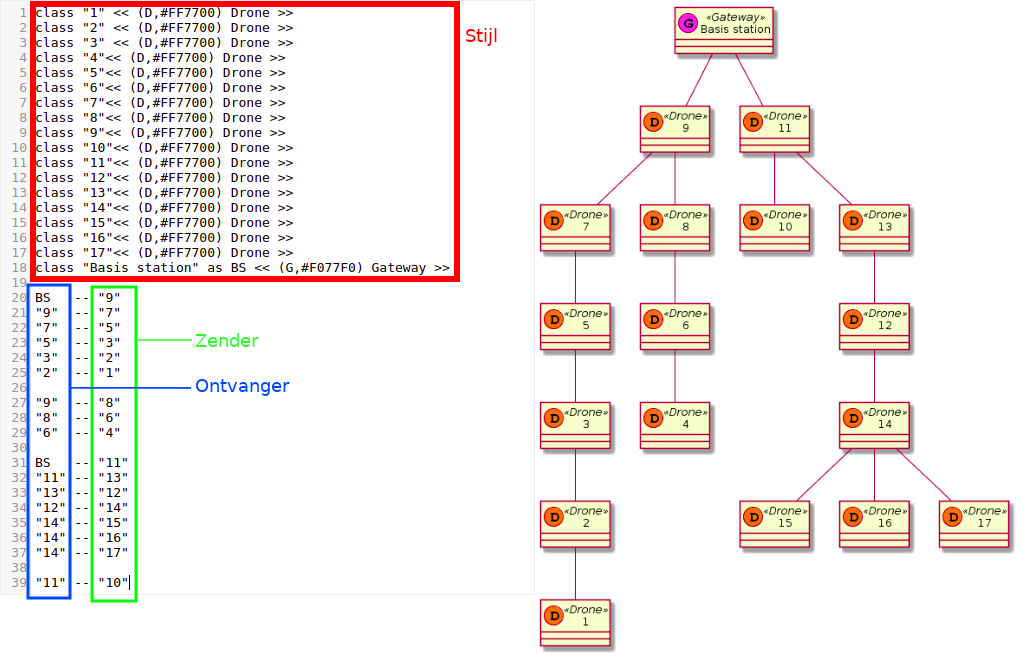
\includegraphics[width=\linewidth]{zenderontvangertopo}\end{center}
	\caption{Topologie van het casusnetwerk door middel van PlantUML.}
	\label{fig:toplogienetwerkuml}
\end{figure}


\subsubsection{Conclusie}  
Het ID van de ontvanger zit al in het bericht aangezien deze de opsteller van het bericht is.
Dit houdt in dat enkel een ID toegevoegd hoeft te worden van de aangemelde zender.
De byte grootte van de ID's is al bekend deze telt namelijk 1 byte.
Daarmee zou het bericht het volgende format krijgen te zien in \autoref{tab:topologiemessage}.

\begin{table}[H]
	\centering
\begin{tabular}{l|l|l|l|}
	\cline{2-4}
	& \cellcolor[HTML]{C0C0C0}ID & \cellcolor[HTML]{C0C0C0}\begin{tabular}[c]{@{}l@{}}Bericht \\ type\end{tabular} & \cellcolor[HTML]{C0C0C0}ZenderID  \\ \hline
	\multicolumn{1}{|l|}{\cellcolor[HTML]{C0C0C0}\begin{tabular}[c]{@{}l@{}}			Aantal\\ Bytes\end{tabular}} & 1   & 1  & 1  \\ \hline
\end{tabular}
	\caption{Berichtsamenstelling aanmelding zender voor topologie.}
	\label{tab:topologiemessage}
\end{table}
Dit houdt in dat dit bericht een totaal van 3 bytes telt.

\subsection{Conclusie}
\label{sec:payloadconclusie}

In deze paragraaf wordt antwoord gegeven op de vraag: Wat is de grootte van de payload die een netwerkmodule aangesloten op een drone moet versturen om nuttig te zijn voor het aansturingssysteem?
Er is gekeken hoe het bericht opgesteld moet worden en naar de inhoud van twee verschillende berichten die relevant zijn voor het aansturingssysteem.
Het grootste bericht van deze twee was het bericht waar in staat op welke positie de netwerkmodule zich bevindt.
Dit bericht telt 17 bytes en is een bericht die informatie bevat van vier verschillende waardes.
Hoewel er meer berichten zullen bestaan in het netwerk is het onaannemelijk dat deze groter zullen zijn dan deze 17 bytes.
Om toch ruimte te houden voor extra informatie in een bericht voor bijvoorbeeld data verificatie worden er 4 bytes toegevoegd aan het maximum. 
Dit zou voldoende ruimte moeten geven doordat er één 32 bits waarde of twee 16 bits waardes toegevoegd kunnen worden.

Daarmee is de conclusie dat de maximale grootte 21 byte is voor een bericht om nuttig te zijn voor een aansturingssysteem.

\section[Welke meshnetwerk hardware?]{Welke meshnetwerk hardware is geschikt voor het onderling verbinden van drones?}
\label{sec:meshnetwerkkeuze}

Om een onderling netwerk op te bouwen is hardware nodig. 
Deze hardware moet voldoen aan de gestelde \nameref{chapter:criteria} zodat het geschikt is voor een drone netwerk.
In \autoref{sec:payloadconclusie} is vastgesteld dat de payload berichten van 21 byte moet kunnen bevatten.
Criteria \hyperlink{ph1}{PH1} eist dat het bereik van de modules minimaal 500 meter is.
Vervolgens stelt criteria \hyperlink{ph5}{PH5} stelt dat het netwerk zuinig in gebruik moet zijn. 

\subsection{Wat is een meshnetwerk?}
\label{sec:meshnetwerkkeuze:watismesh}
Een meshnetwerk is een term die gebruikt wordt voor een topologie techniek in netwerken.
Om een voorbeeld beter toe te kunnen lichten worden eerst de tegenhangers besproken de ster en boom topologie.

Een doorsnee huishouden maakt zeer waarschijnlijk gebruik van een ster topologie.
Er staat een modem bij de aansluiting in het huis die een Wifi signaal uitzendt.
Alle mobiele apparaten kunnen hiermee verbinden en er zijn vaak nog een fysieke poorten voor een bekabelde verbinding.
Dat levert een topologie op zichtbaar in \autoref{fig:toplogiester}.

\begin{figure}[H]
	\begin{center}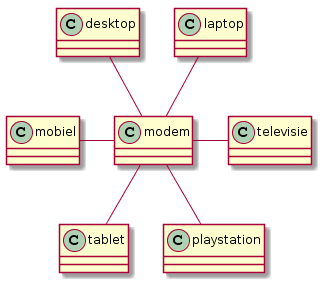
\includegraphics[width=.4\linewidth]{sterTopo}\end{center}
	\caption{Topologie van ster netwerk.}
	\label{fig:toplogiester}
\end{figure}

In de meeste huishoudens volstaat dit aangezien de router bereikbaar is vanaf elk punt in het huis.
Op het moment dat dit niet zo is het gangbaar om uit te wijken tot een boom topologie door een of meerdere routers toe te voegen in het netwerk.
Vertaalt naar een topologie zou dit er als \autoref{fig:toplogieboom} uitzien.

\begin{figure}[H]
	\begin{center}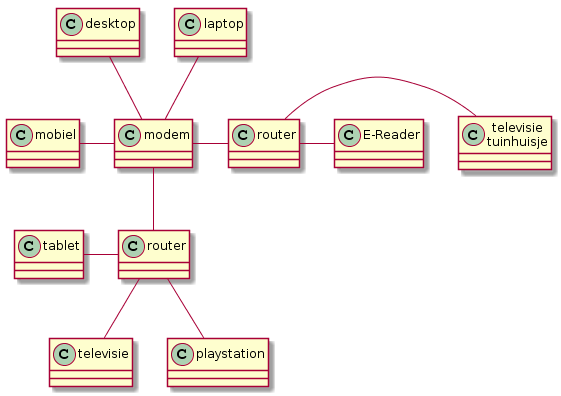
\includegraphics[width=.5\linewidth]{treeTopo}\end{center}
	\caption{Topologie van boom netwerk.}
	\label{fig:toplogieboom}
\end{figure}

Een probleem wat uit deze twee voorbeelden duidelijk wordt is de grens van het bereik. 
Deze is namelijk alleen uit te breiden door het toevoegen van extra netwerkpunten.
De meshnetwerk techniek is een oplossing voor dit probleem.
In een meshnetwerk zijn de apparaten in staat om direct met elkaar te verbinden. 
Zo is elk apparaat in het netwerk direct een uitbreiding in het bereik van het netwerk doordat het informatie kan doorgeven.

Er zitten aan een meshnetwerk ook nadelen.
Omdat er nu meerdere routes van en naar een apparaat zijn komt er een extra protocol bij kijken welke route genomen moet worden wat extra complexiteit toevoegt.
Daarnaast zal het draadloze verkeer verhoogt worden waardoor uiteindelijk apparaten elkaar zullen verstoren.
Tenslotte voegt het ook een afhankelijkheid toe, omdat bijvoorbeeld de televisie in het tuinhuisje de laptop in de keuken gebruikt als stap naar het modem.

\begin{figure}[H]
	\begin{center}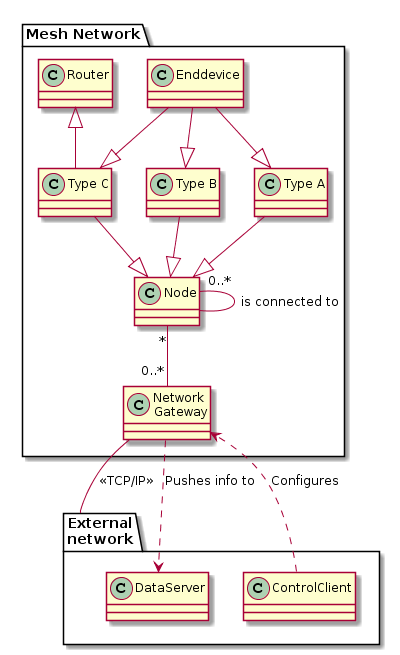
\includegraphics[width=.3\linewidth]{meshclass}\end{center}
	\caption{Verbanden tussen de rollen in een meshnetwerk.}
	\label{fig:meshrol}
\end{figure}

In een meshnetwerk zijn er twee rollen te verdelen \cite{compNRF}.
Er is de rol van gateway waarmee het netwerk verbonden wordt naar een extern punt. 
En er is de rol van node welke in staat is om met een gateway te verbinden of met een andere node.

Een node is vervolgens weer te verdelen in drie types, de namen die hier aan gegeven worden verschillen per aanbieder voor het gemak worden die van LoRa gebruikt.
In LoRa wordt gesproken over type A, B en C waarbij elke type gericht is op een verschillende visie van stroomconsumptie \cite{LoraLimit}.

\begin{itemize}
	\item \textbf{Type A} is de energiezuinigste variant doordat het alleen online komt op het moment dat het data moet versturen.
Een nadeel hieraan is  dat het communiceren naar dit type node onmogelijk is en het dus ook niet bijdraagt het uitbreiden van het netwerk.
	\item \textbf{Type B} is een variant van type A welke na het zenden van een bericht enige tijd online blijft om een berichten te kunnen ontvangen. 
Een voordeel is dat deze dus wel op afstand aan te sturen is maar nog steeds is deze alleen een gebruiker van het netwerk.
	\item \textbf{Type C} is de minst zuinige variant van de nodes, omdat hij altijd aan staat.
Het nadeel is dat deze node het meest stroom verbruikt. Daarin tegen kan deze node wel de belangrijke rol krijgen van router en vergroot daarmee het bereik van het meshnetwerk.
\end{itemize}

In het geval van de opdracht wordt alleen gekeken naar type C nodes, omdat er interesse is naar de dynamische plaatsing van dit type.




\subsection{Keuze in LPWAN hardware}
De gestelde eisen over bereik en energieverbruik zijn een logische stap om een verdieping uit te voeren in low-power wide-area network (LPWAN) netwerken. 

In de publicatie van \cite{LoraConnect} wordt het LoRaWAN netwerk onderzocht.
Ook worden daar de grootste concurrenten van het LoRaWAN netwerk benoemd namelijk SigFox \citeyear{sigfox} en Narrowband IoT (NB-IoT).
Ondanks het feit dat deze protocollen niet interessant zijn voor het project, omdat ze in de verkeerde OSI-laag vallen, is de netwerklaag wel interessant om te bekijken welke technieken er gebruikt worden.
NB-IoT valt direct af als oplossing doordat het gebruikt maakt van mobiele communicatie en dus niet zou voldoen aan criteria \hyperlink{ph4}{PH4}.
SiGFox valt ook af, omdat het gebruik maar beperkt openbaar is gemaakt. Om deze reden is het niet geschikt is om een meshnetwerk mee te bouwen. 
Dan blijft uit deze publicatie het LoRaWAN netwerk over. 

\subsubsection{LoRa}
Het LoRaWAN netwerk is gebaseerd op de LoRa fysieke laag (PHY) \cite{LoRAMOD} implementatie om de communicatie af te handelen.
LoRaWAN is een netwerkstandaard opgezet voor telecom providers om het mogelijk te maken netwerken op te zetten voor communicatie over afstanden tot \SI{15}{\kilo\meter}.
Alleen het LoRaWAN maakt gebruikt van een ster topologie doordat nodes maar één hop kunnen maken naar een gateway van het netwerk.
Een andere nadeel die het LoRa netwerk heeft, is dat ondanks de grote afstand die het kan afleggen door de spreidingsfactor te vergroten en de gevoeligheid van de ontvanger te verhogen, dit ten koste gaat van de snelheid van de datadoorvoer.
\citeA{LoraMesh} hebben onderzoek gedaan naar de mogelijk om het LoRa PHY netwerk te gebruiken als meshnetwerk en ook aangetoond dat dit werkt.
Het doel van hun onderzoek was om door middel van meshtechnieken LoRa geschikter te maken voor verstedelijkt gebied zonder het toevoegen van extra gateways. 
Een nadeel wat ze beschrijven in de conclusie is het aantal nodes wat ze kunnen verwerken verkleind wordt.
Dit komt door de degradatie van timing prestaties waarin ze stellen dat periode $p$ die een bericht nodig heeft om verstuurd te worden naar de gateway de volgende regel volgt ($p = 2h\cdot t$) waarbij $h$ het aantal hops is die het bericht maakt en $t$ de frametijd. Om de frametijd te berekenen geldt het volgende: $frametijd = \frac{framelengte}{bitsnelheid}$. 
Een voordeel van het gebruik die een mesh kan hebben ten opzichte van een ster netwerk is dat het een hogere bitsnelheid kan behouden. Dit kan een mesh omdat er kleinere afstanden overbrugt hoeven te worden waardoor de frametijd alsnog klein kan blijven.
Een voorwaarde van het gebruik van dit netwerk is dus wel dat de framelengte klein moet zijn waardoor het niet geschikt is voor het verwerken van grote berichten zoals afbeeldingen, video of andere grote bestanden.

\paragraph{LoRa samengevat}
\citeA{LoraMesh} hebben al aangetoond dat een meshnetwerk op basis van LoRa mogelijk is waardoor het risico afneemt in de haalbaarheid van dit onderzoek.
Een voordeel van dit netwerk is de afstand die de netwerkmodules van elkaar kunnen staan die met deze techniek kan oplopen tot meer dan 10 kilometer afhankelijk van de hoeveelheid en frequentie van de data die verstuurd moet worden.
Een ander voordeel van deze techniek is dat het signaal enorme afstanden kan halen bij een vrije line of sight waarbij het wereldrecord zelf op 702 kilometer staat door een weerballon op 38 kilometer hoogte te gebruiken \cite{LoRARecord}.
Hoewel deze extreme usecase niet zal voorkomen worden de netwerk modules wel gemaakt om aan drone gekoppeld te worden.
Hierdoor is het makkelijk mogelijk voor een netwerkmodule om geplaatst te worden op hoge punten. 
Een nadeel van dit netwerk is de lage data snelheid waardoor het alleen geschikt is voor toepassingen die weinig data versturen zoals sensor netwerken.

\subsubsection{nRF24l01+}\label{sec:nrf24l01}
De nRF24l01 long range is een transciever van Nordic Semiconductor die werkzaam is op de 2,4ghz band \cite{nRFspec}.
De module kan gebruik maken van verschillende standen van datasnelheid: \SI{250}{\kilo\bit\per\second}, \SI{1}{\mega\bit\per\second}, \SI{2}{\mega\bit\per\second}.
Hoewel het een 3,3 volt apparaat is zijn de I/O pinnen 5 volt tolerant waardoor het een veilige interface biedt aan microcontrollers. Daarnaast is door het aanbod van 3,3 volt I/O geschikt voor het gebruik op een Raspberry Pi.

Er zijn van de module twee varianten met een gelijke interface. 
Er is een module (nRF24l01) voor korte afstand en een module (nRF24l01+pa+lna) voor lange afstanden vaak aangeduid als nRF24l01+.
De module voor lange afstanden beschikt over een power amplifier en een low noise amplifier wat het een beter zend en ontvangst vermogen geeft.
De module heeft volgens de specificaties een theoretisch bereik van 1100 meter bij vrij zicht.
Er zijn verschillende video's op youtube waar aangetoond wordt dat deze afstand gehaald wordt.
Zo wordt in de video van iforce2d \citeyear{nrfAfstand} een afstand overbrugt van 700m met een data rate van \SI{250}{\kilo\bit\per\second}.
Het zal in ieder geval voldoende zijn om de eis van 500 meter te overbruggen.  

\begin{figure}[H]
	\begin{center}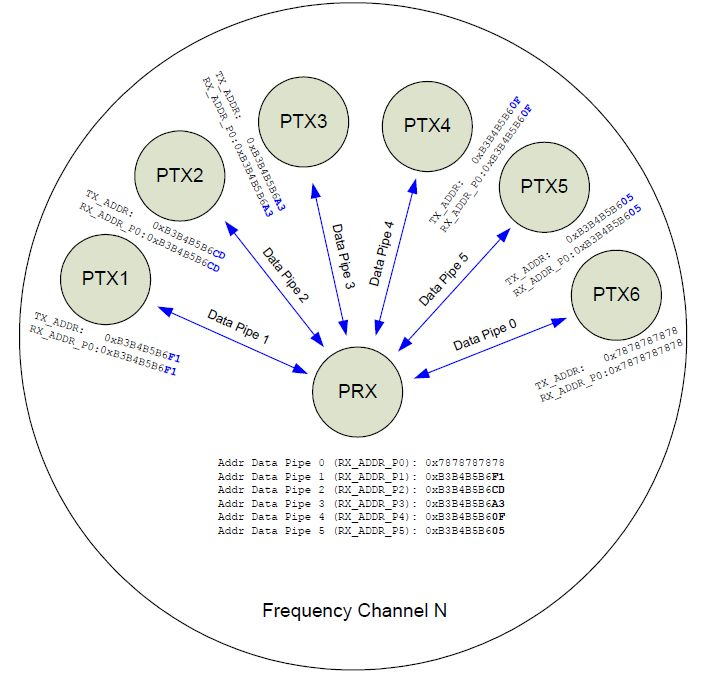
\includegraphics[width=0.4\linewidth]{Afbeeldingen/nrfMulticiever.jpg}\end{center}
	\caption{Werking van verbindingen nRF24l01. Afkomstig van \href{https://www.instructables.com/id/NRF24L01-Multiceiver-Network}{https://www.instructables.com/id/NRF24L01-Multiceiver-Network}, 18 maart 2019.}
	\label{fig:nrfchannel}
\end{figure}
De nRF24l01+ kan tot zes adressen tegelijk onderhouden die kunnen schakelen tussen een RX (ontvang) en TX (zend) stand. 
\autoref{fig:nrfchannel} laat het gebruik van adressen zien, hierin is te zien dat een adres is opgebouwd uit 5 bytes.
Dit levert een totaal op van 10782039375 ($255^{5}$) unieke adressen.
Het grote aantal zal waarschijnlijk nooit bereikt worden door de complexiteit die de topologie van een dusdanig netwerk geeft.
De modules versturen pakketten met een maximale grootte van 32 byte.


Als er gekeken wordt naar de populaire libary genaamd nRF24 dan wordt er gebruikt gemaakt van 1 byte voor het adres wat 255 unieke mogelijkheden geeft.
De samenstelling van een pakket is af te lezen in \autoref{tab:nrf} \nameref{tab:nrf}

\begin{table}[H]
	\centering
	\begin{tabular}{l|l|l|l|l|l|}
		\cline{2-6}
		& \cellcolor[HTML]{C0C0C0}FROM & \cellcolor[HTML]{C0C0C0}\begin{tabular}[c]{@{}l@{}} TO\end{tabular} & \cellcolor[HTML]{C0C0C0}FORWARD & \cellcolor[HTML]{C0C0C0}ACK & \cellcolor[HTML]{C0C0C0}PAYLOAD \\ \hline
		\multicolumn{1}{|l|}{\cellcolor[HTML]{C0C0C0}\begin{tabular}[c]{@{}l@{}}Aantal\\ Bytes\end{tabular}} & 1                          & 1                                                                               & 1                                & 1                                 & 28                                                          \\ \hline
	\end{tabular}
	\caption{NRF24 libary pakket.}
	\label{tab:nrf} 
\end{table}

In deze toepassing blijft er dus ruimte over voor 28 bytes als payload wat nog steeds voldoende zou zijn voor de netwerkmodules van de drones.


\subsubsection{Conclusie keuze hardware: LoRa vs nRF}

Er zijn nu twee kandidaten voor het netwerk.
De LoRa PHY module die gigantische afstanden kan afleggen maar als keerzijde een langzame verbinding heeft.
Als andere kandidaat is er de nRF24l01+ een module die vele malen sneller is maar dan ook flink inlevert op het bereik ten opzichte van LoRa.

Omdat beide modules voldoen aan de gestelde eisen en in staat zijn de gewenste payload te versturen zijn ze voorgelegd aan de technisch manager van Alten Nederland.
Hij ziet een betere business case in een netwerk met een hogere dichtheid maar dan ook een hogere snelheid.
Daarom zal er in dit project gebruik gemaakt worden van de nRF24l01+.


\section[nRF24 met Raspbery Pi Model B+]{Aansturing nRF24 met een Raspbery Pi Model B+}

\autoref{sec:meshnetwerkkeuze} heeft als uitkomst gegeven dat er voor de communicatie een nRF24l01+ gebruikt moet worden.
Deze moet alleen ook aangestuurd worden en dit kan op verschillende manieren.
Voor nu heeft Alten aangegeven dat zij graag wil dat dit gedaan wordt op een Raspbery Pi Model 2B+.
Deze heeft Alten al beschikbaar en wil eerst weten of het mogelijk is op een Raspbery Pi.
Als dit mogelijk is wil Alten pas gaan investeren in ontwikkeling op een microcontroller.
De ontwikkeling op een Raspberry Pi model 2B+ sluit aan op de requirements gesteld aan het project en wordt op wens van de student uitgevoerd in C++.


\section[Welke routeringstechniek?]{Welke routeringstechniek is geschikt voor de te gebruiken hardware?}
\label{sec:meshnetwerktechniek}

Het netwerk wordt opgebouwd door het toepassen van een meshnetwerktechniek.
Wat een meshnetwerk is, wordt toegelicht in \autoref{sec:meshnetwerkkeuze:watismesh}.
Een kenmerkend eigenschap van een meshnetwerk is het hebben van meerdere verbindingspunten per router of gateway.
Dit wordt opgezet door een routeringstechniek.
Er zijn verschillende technieken met elk voor en nadelen.
De technieken zijn te verdelen in drie groepen: proactief, reactief en hybride \cite{meshprotocols}.
Het verschil tussen deze technieken zit in hoe routes naar andere nodes in het netwerk toe gevonden worden.
In de hierop volgende paragrafen worden deze technieken kort toegelicht. 
Afsluitend zal besloten worden welke van deze drie het meest geschikt is voor de te gebruiken hardware.


\begin{figure}[H]
	\begin{center}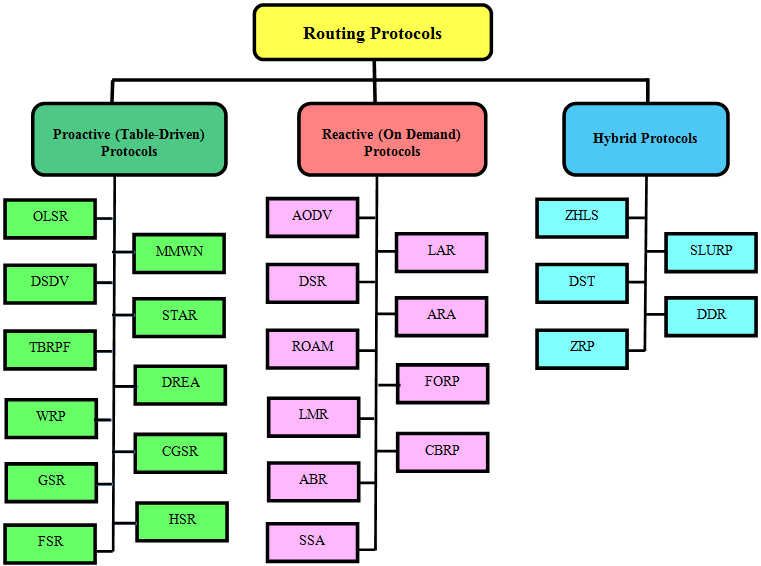
\includegraphics[width=0.6\linewidth]{Afbeeldingen/meshprotocollen.png}\end{center}
	\caption{Bestaande routeringsprotocollen. Afkomstig van \protect\cite{meshprotocols}.}
	\label{fig:meshprotcollen}
\end{figure}

\subsection{Proactieve routeringstechniek}
\label{sec:meshnetwerktechniek:proactief}

Een proactief protocol is een protocol die zelf constant bezig is met het zoeken naar nieuwe punten in het netwerk.
De nodes zorgen dat veranderingen meteen kenbaar gemaakt worden aan andere punten in het netwerk. 
Dit zorgt ervoor dat het netwerk een zelf herstellend vermogen heeft en geschikt is voor het opsporen van fouten in het netwerk.
Het protocol is geschikt voor situaties waar de posities van nodes zelden tot nooit veranderen. 
In situaties waar paden vaak veranderen door het veranderen van node posities zal het protocol veel meer bandbreedte vragen van het netwerk. 

\begin{figure}[H]
	\begin{center}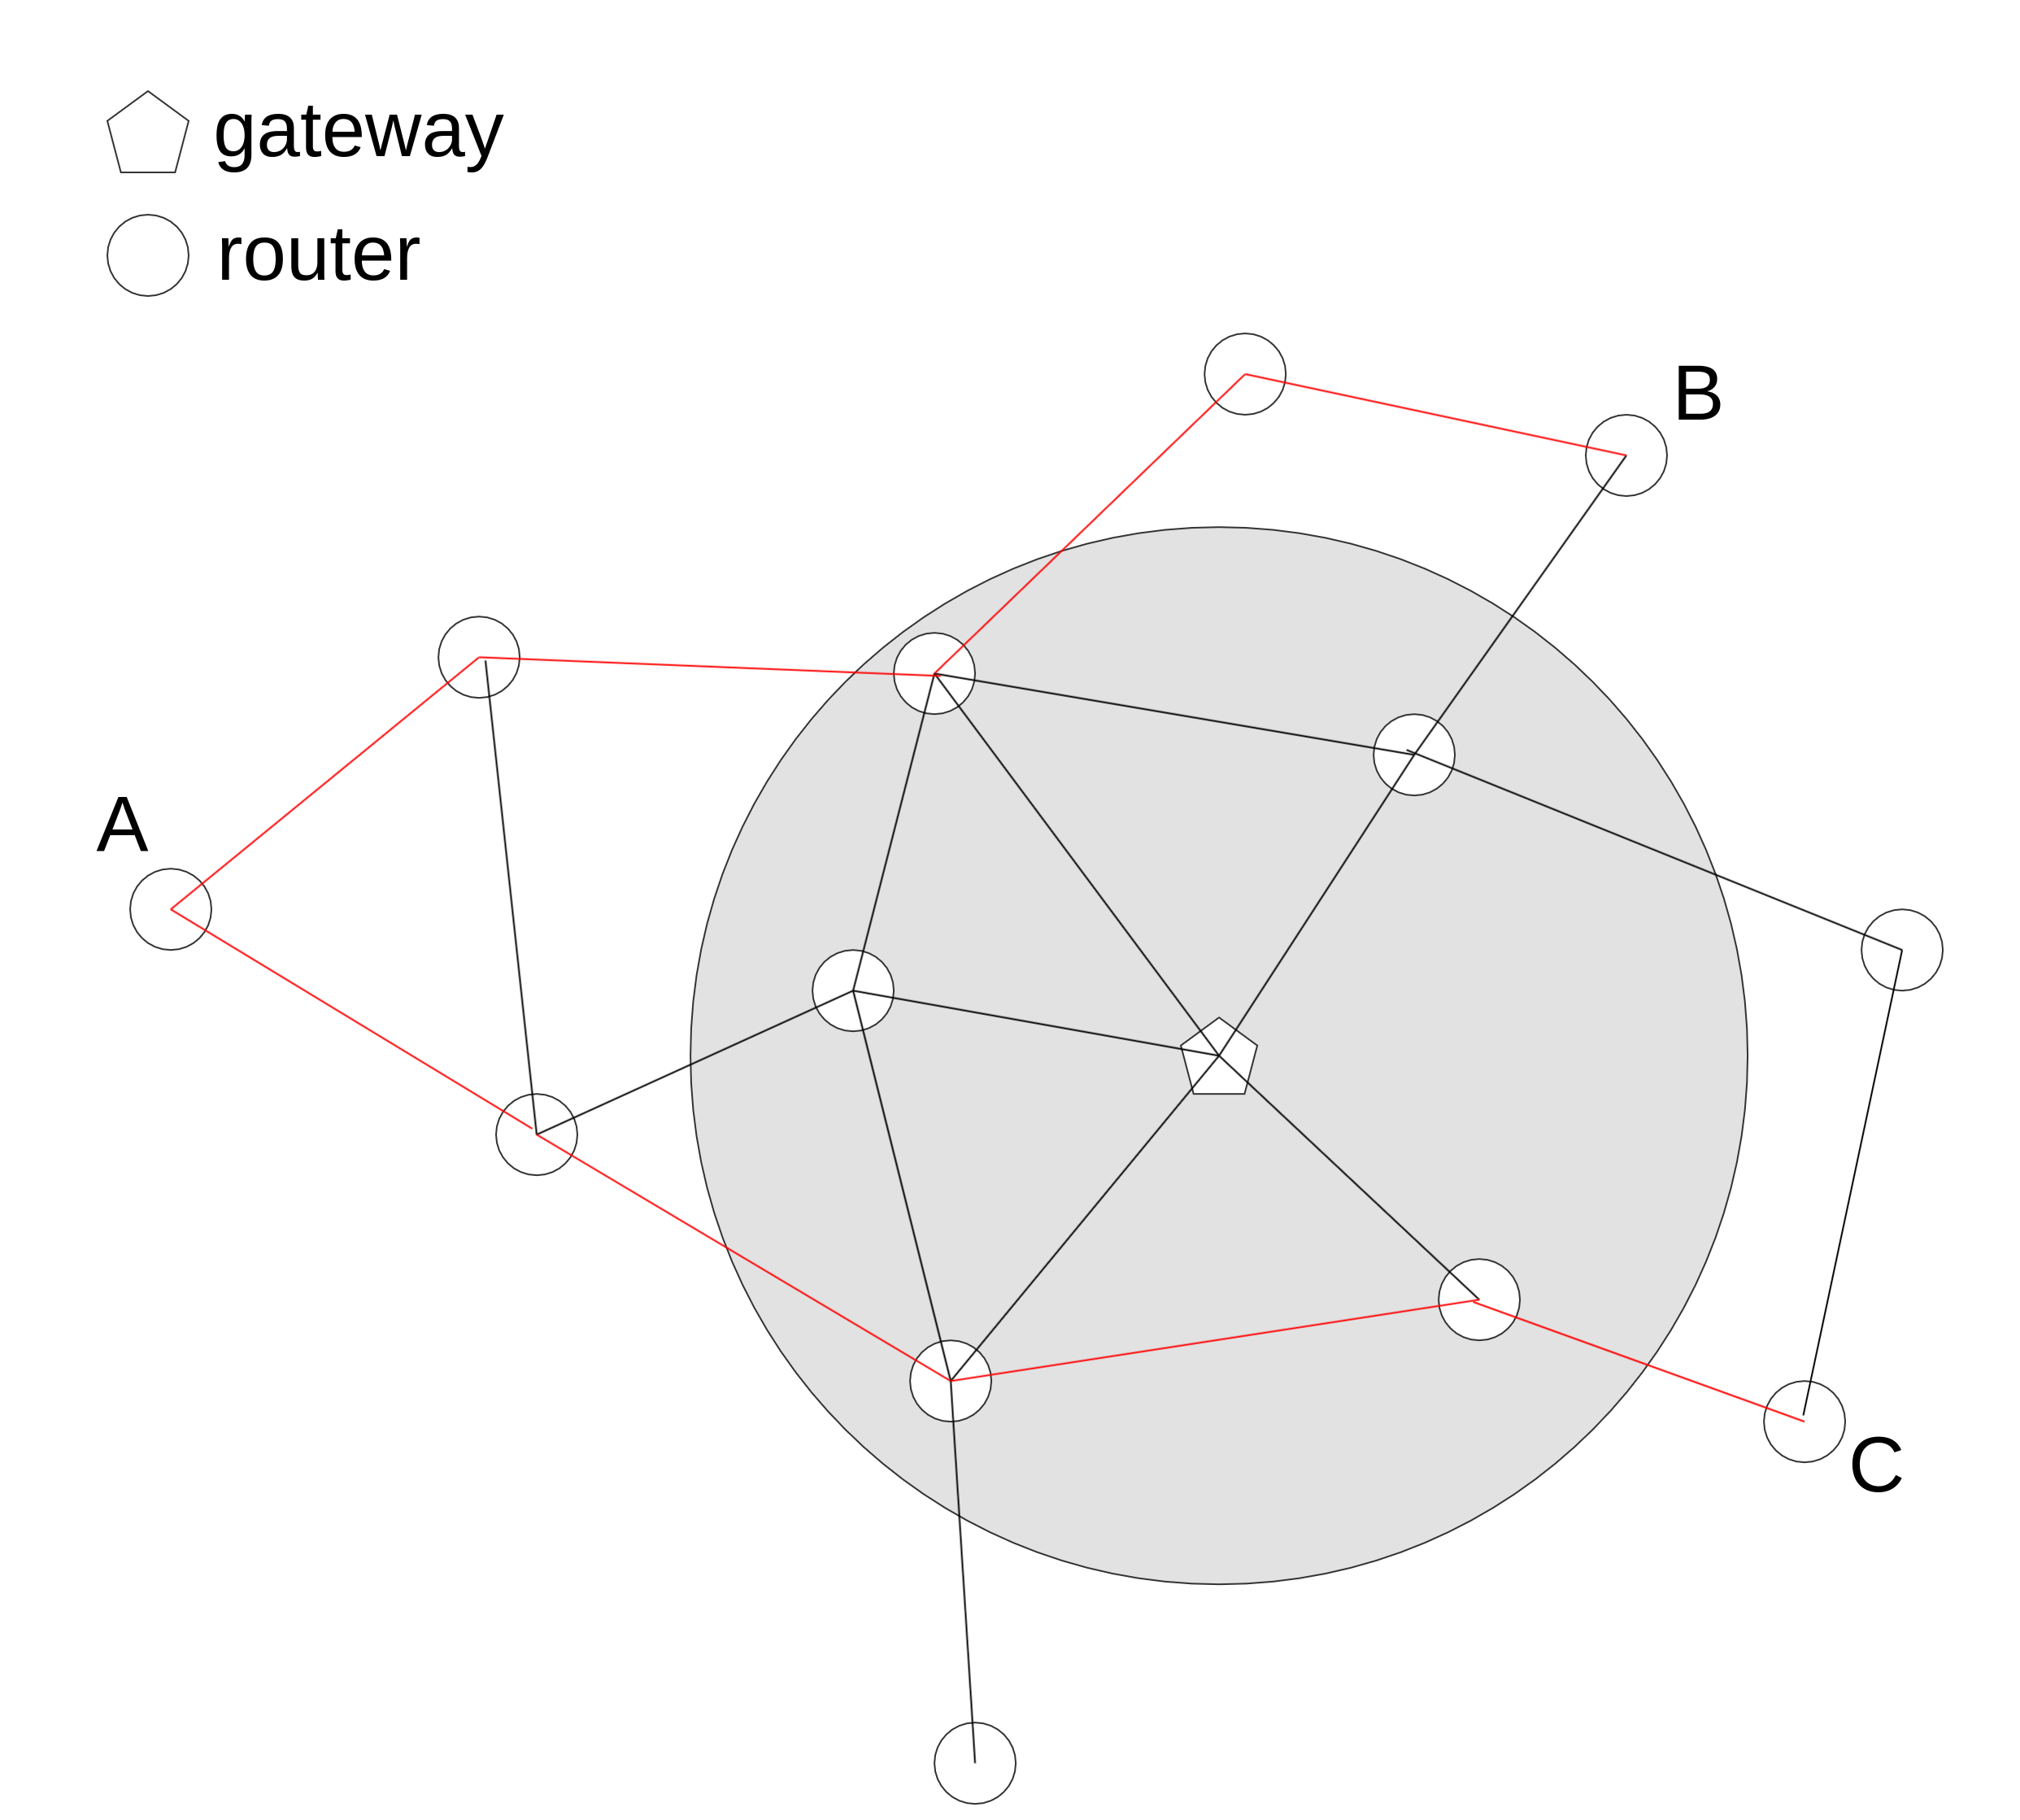
\includegraphics[width=0.45\linewidth]{Afbeeldingen/proactive.png}\end{center}
	\caption{Voorbeeld proactieve routeringstechniek.}
	\label{fig:proactief}
\end{figure}

In \autoref{fig:proactief} wordt een voorbeeld getoond waar punt A een bericht wil versturen naar punt B en C. 
Punt A en alle andere punten in het netwerk zijn op de hoogte van alle routes in het netwerk.
In de huidige situatie zijn er 21 verbindingen in het netwerk tussen de nodes.
Er zijn 14 punten aanwezig in het netwerk minimaal zullen er dus voor het op de hoogte brengen van bestaande verbindingen 294 ($14 \times 21$) berichten rondgestuurd moeten worden. 

Na introductie kan er een pad gemaakt worden waarover een bericht verstuurd kan worden.
Dit voorbeeld laat goed zien dat deze routingstechniek zijn voordeel haalt wanneer de nodes stil blijven staan, omdat er dan niet opnieuw berichten verstuurd hoeven te worden. 
 
\subsection{Reactieve routeringstechniek}
\label{sec:meshnetwerktechniek:reactieve}

Een reactieve routeringstechniek is een methode waarbij de nodes geen routes opslaan maar op aanvraag routes opbouwen. 
Dit scheelt in het gebruik van geheugen en het gebruikt minder berichten bij het initialiseren van het netwerk. 
Daarentegen kost het deze techniek meer tijd om een bericht te versturen.
Het kost meer tijd omdat er voordat er een bericht verstuurd kan worden eerst een route opgebouwd moet worden.

\begin{figure}[H]
	\begin{center}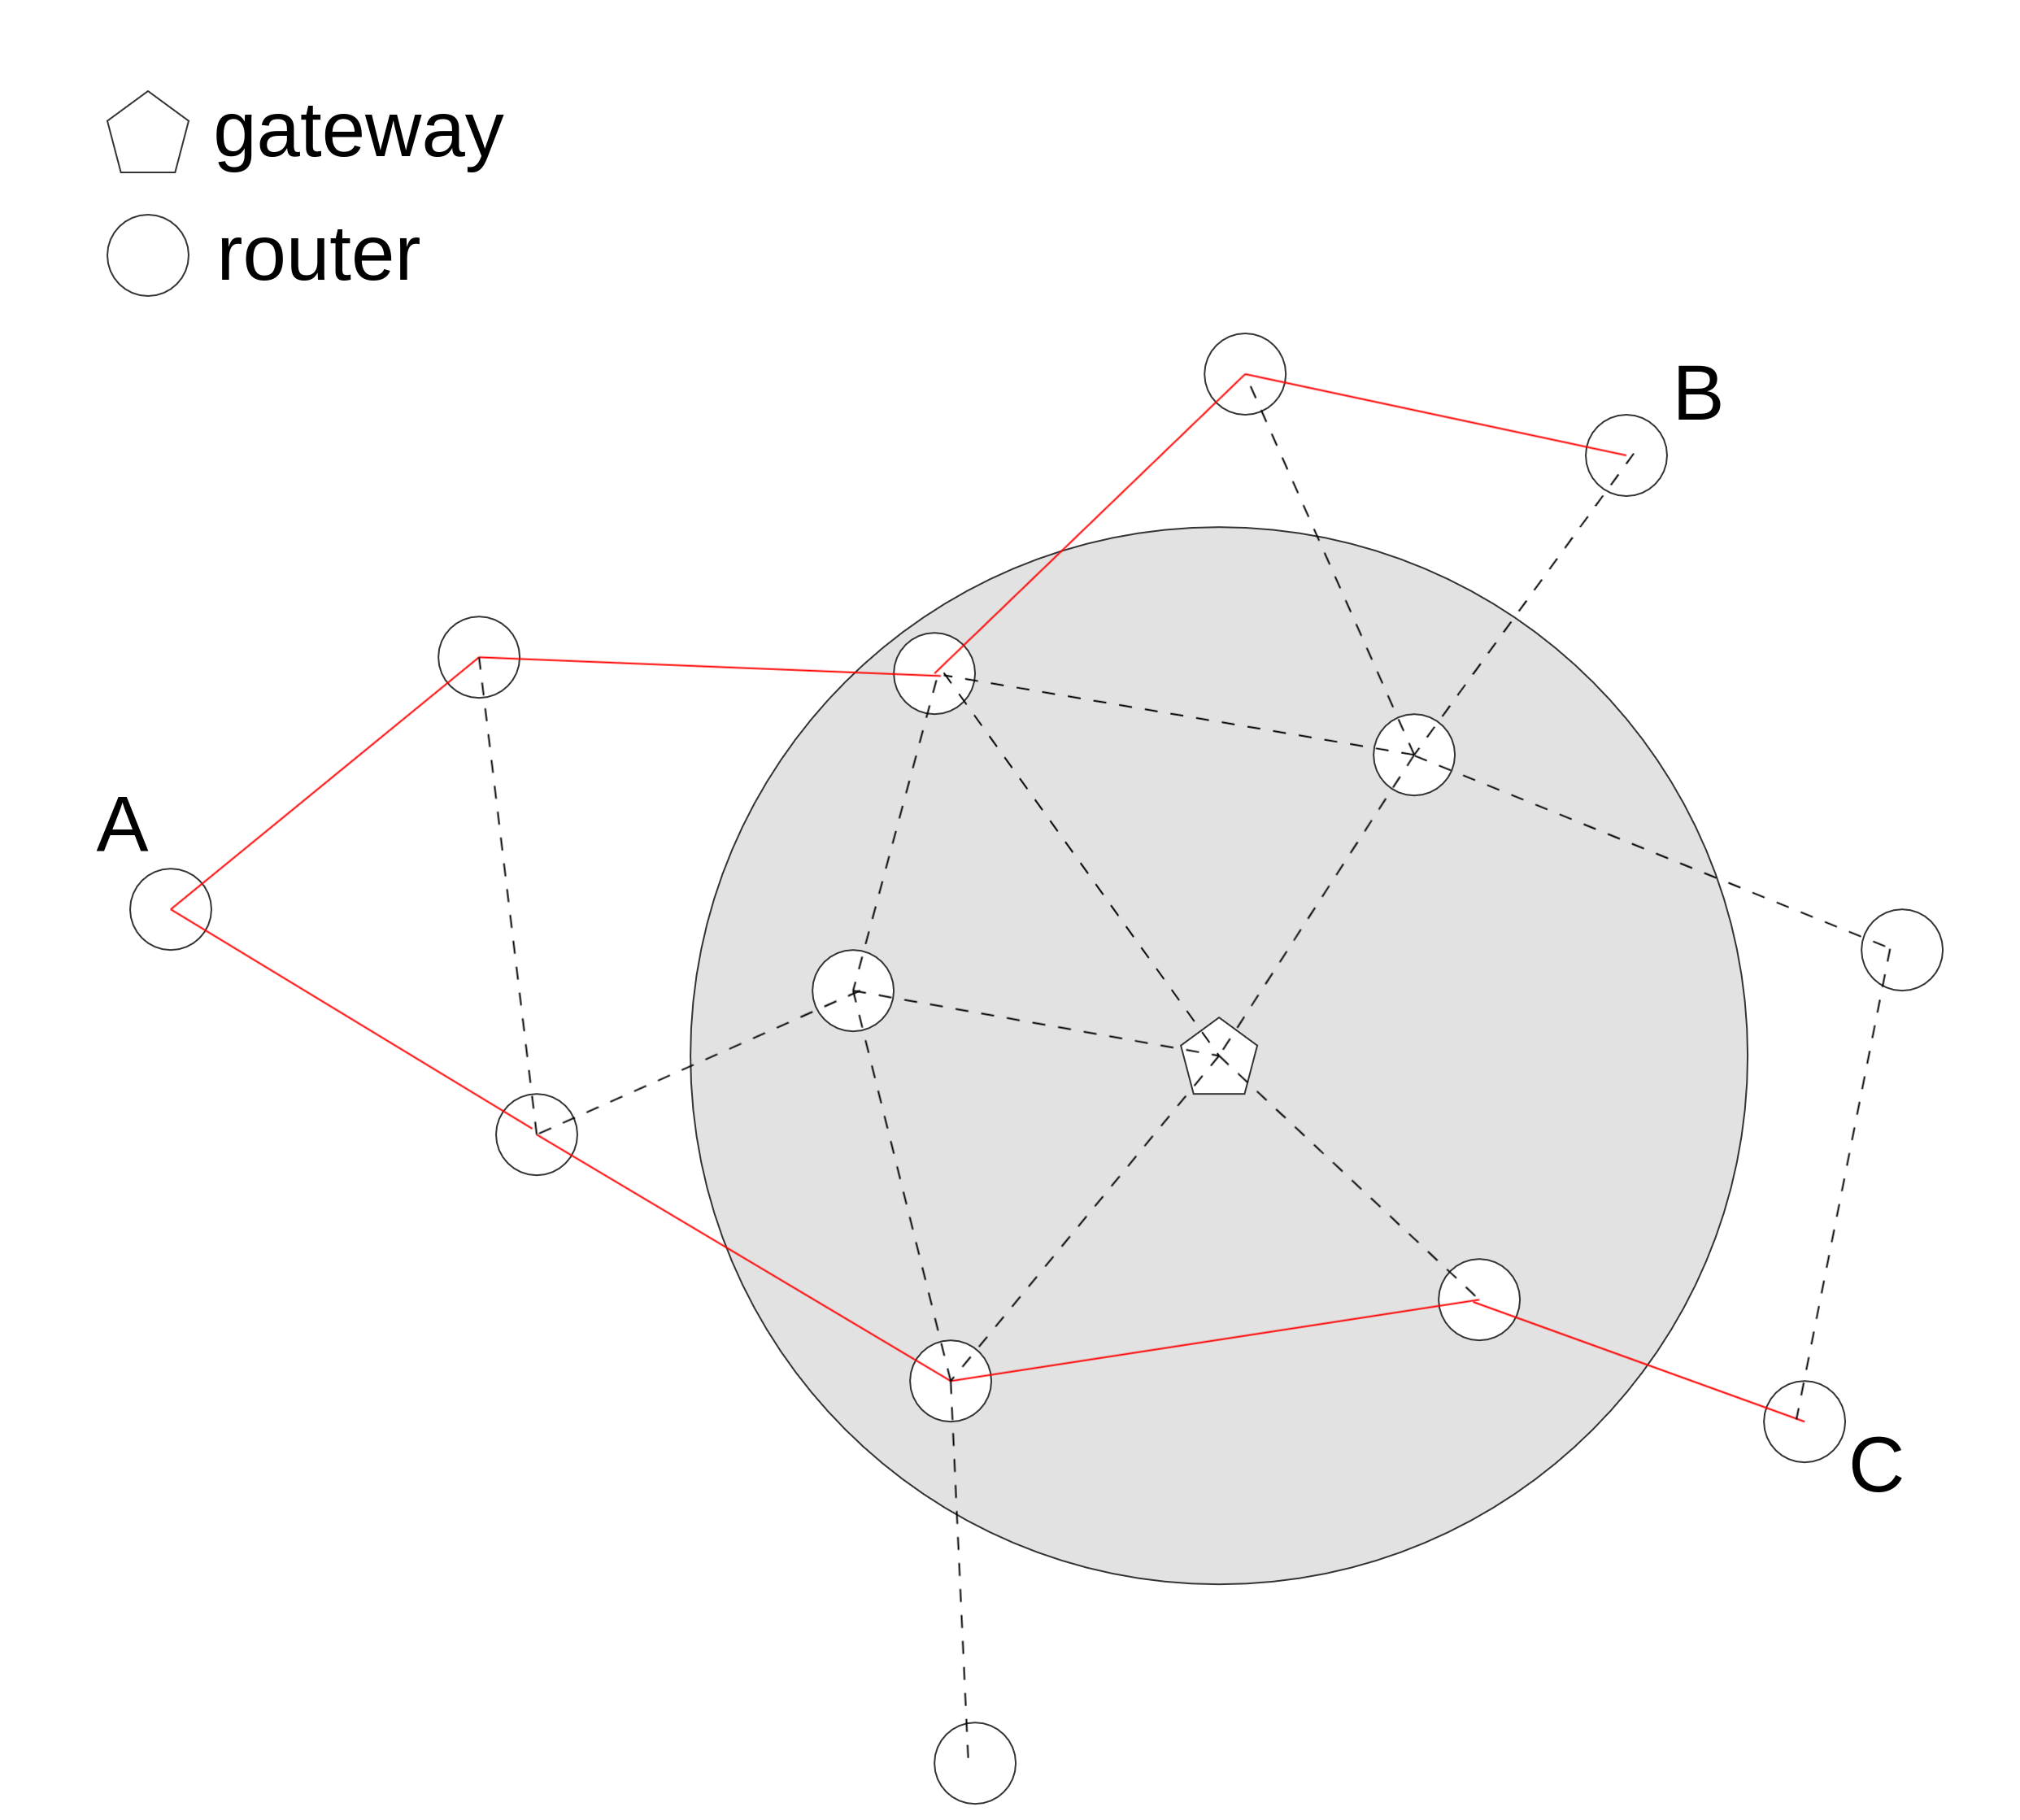
\includegraphics[width=0.45\linewidth]{Afbeeldingen/reactive.png}\end{center}
	\caption{Voorbeeld reactieve routeringstechniek.}
	\label{fig:reactief}
\end{figure}

\autoref{fig:reactief} laat een voorbeeld zien waarin er gebruik gemaakt wordt van een reactieve routeringstechniek.
Er zal in dit voorbeeld, voordat een route gezocht wordt, een route gemaakt moeten worden tussen de twee punten.
Vervolgens als deze route gevonden is zal er een bericht hierover gestuurd worden. 
Deze route wordt tijdelijk opgeslagen tot de node klaar is met het versturen van zijn data.

\subsection{Hybride routeringstechniek}
\label{sec:meshnetwerktechniek:hybride}
Een hybride routeringstechniek is een techniek die een proactieve en reactieve techniek deels combineert om zo ongewenste nadelen te elimineren van elkaar. 

\begin{figure}[H]
	\begin{center}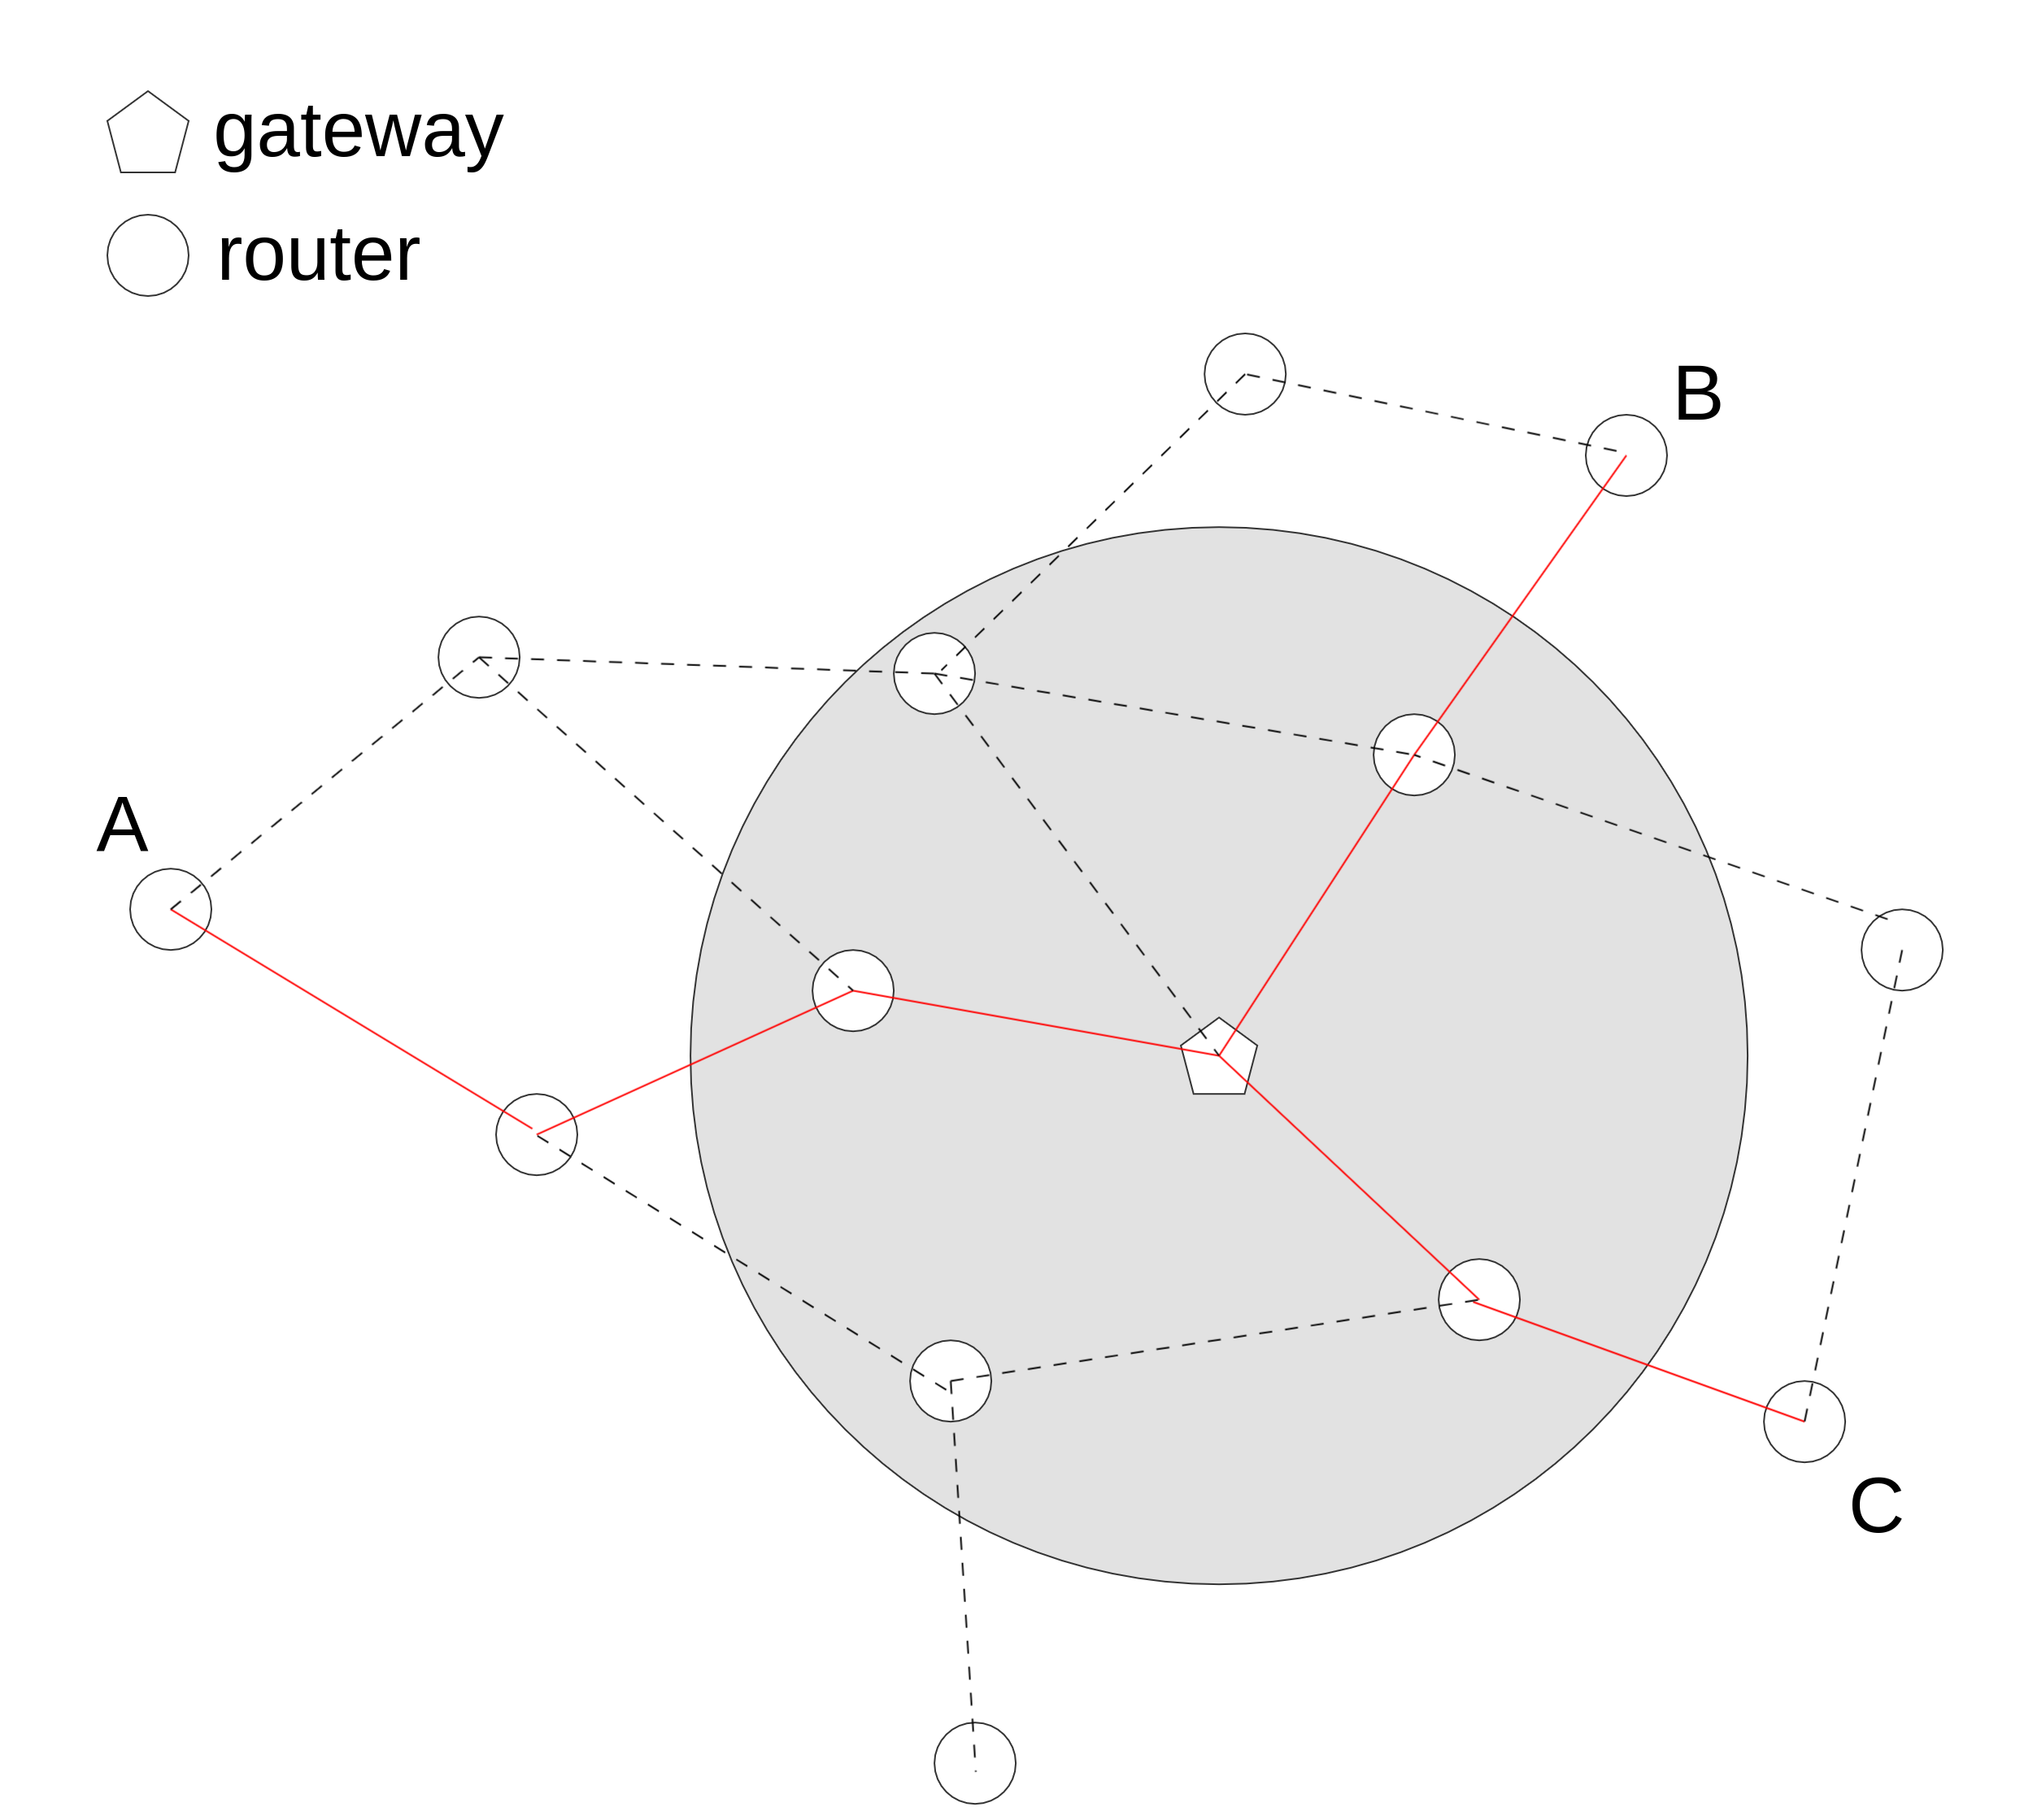
\includegraphics[width=0.45\linewidth]{Afbeeldingen/hybride.png}\end{center}
	\caption{Voorbeeld hybride routeringstechniek.}
	\label{fig:hybride}
\end{figure}

In dit voorbeeld is een hybride routeringstechniek uitgewerkt.
Er zijn veel meer varianten aanwezig.
Het voorbeeld is om te laten zien hoe reactief en proactief gecombineerd kan worden.
In deze situatie is de gateway voorzien van een proactief protocol waardoor het alle routes kent. 
De routers hoeven daardoor alleen een route te bereken naar een gateway toe.   
  
\subsection{Conclusie}
\label{sec:meshnetwerktechniek:Conlusie}
Het dronenetwerk is een netwerk die vaak te maken zal hebben met verplaatsingen.
De hele eigenschap om autonoom nodes te kunnen verplaatsen is zelfs de aanleiding van het project.
Daardoor vallen proactieve routeringstechnieken af. 
Toch is de tegenhanger reactieve routering ook geen ideale oplossing.
Het niet opslaan van routes maakt het versturen van berichten sloom en er is geheugen aanwezig op de microcontroller voor het opslaan van routes. 

Daarom is de conclusie om een zelf een hybride variant te maken van het reactieve Lightweight Mobile Routing(LMR) protocol.
Dit protocol wordt gebruikt, omdat het een protocol is die een hop routeringstechniek gebruikt waardoor de payload klein blijft.
De techniek is niet afhankelijk van een gateway en nodes hoeven alleen te bewust te zijn van de buren en met wie die buren verbonden zijn.
Het protocol hoeft alleen maar aangepast te worden zodat routes opgeslagen blijven.
Doordat deze techniek geen routes hoeft op te slaan van het volledige netwerk  maar alleen die van hun aangesloten buren en hun aangesloten punten zullen er geen grote routeringstabellen gecreëerd worden.

 


\section[minimaal benodigd om een abstracte drone te representeren]{Wat is minimaal benodigd in een simulatie om abstracte drone te representeren?}
\label{sec:dronekeuze}

In \autoref{sec:welkesim} is geconcludeerd dat als simulatiesoftware Ros melodic met Gazebo9 wordt gebruikt.
Hierin kwam naar voren dat niet elke drone package gebruikt kan worden doordat ze specifiek gemaakt zijn voor de versie van Ros.
Omdat het project de focus heeft op de werking van netwerkmodules voldoet een abstracte versie van een drone.
Zo hoeft deze bijvoorbeeld op dit moment nog niet realistisch te vliegen.

Daarom is besloten dat de drone het volgende moet kunnen in de simulatie:

\begin{itemize}
	\item Een drone moet verticaal kunnen opstijgen.
	\item Een drone moet verticaal kunnen landen.
	\item Een drone moet zich kunnen voortbewegen.
	\item Een drone verplaatsing begint altijd met opstijgen en eindigt altijd met een landing.
	\item Een drone moet voorzien zijn van module die een locatie kan teruggeven. 
	\item Een drone mag een basisvorm gebruiken om zich zichtbaar te maken in de simulatie
\end{itemize}

\begin{figure}[H]
	\begin{center}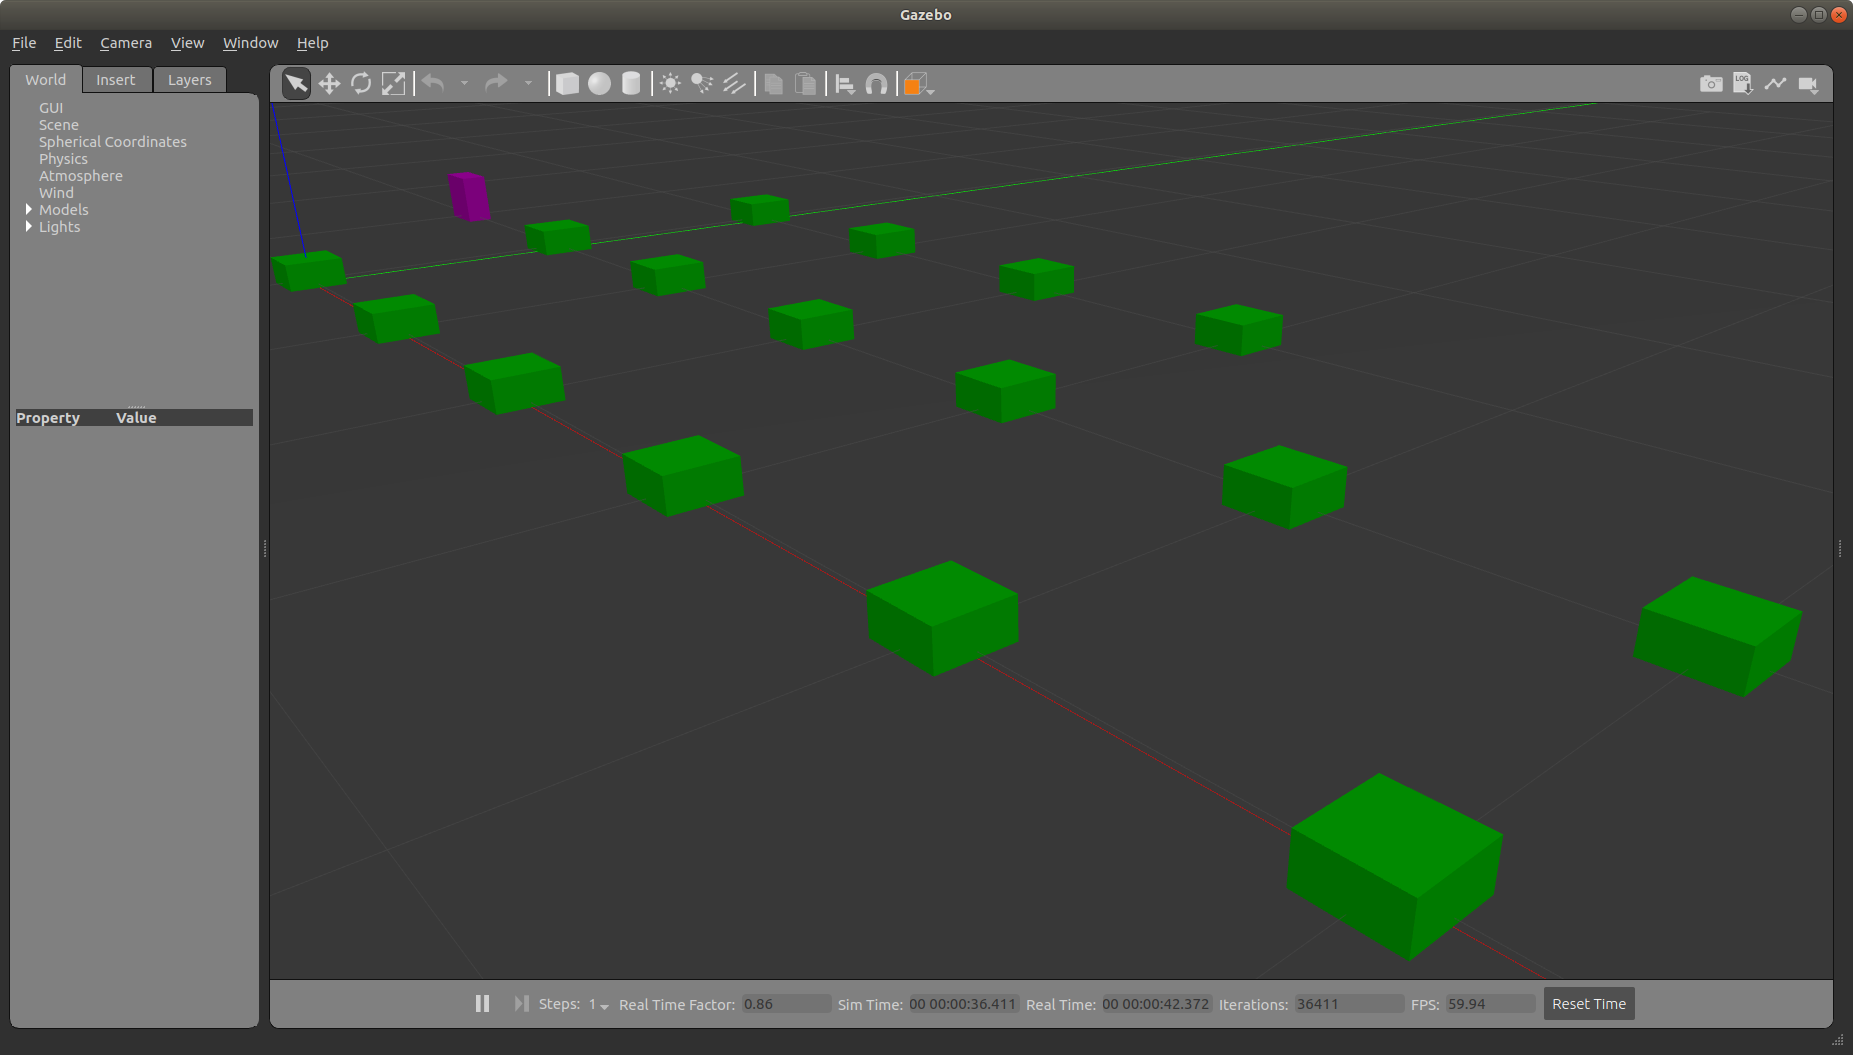
\includegraphics[width=0.45\linewidth]{Afbeeldingen/dronegroep.png}\end{center}
	\caption{Groep van drones in de simulatie.}
	\label{fig:abstractdrones}
\end{figure}


\chapter{Oplossingsrichtingen}

In dit hoofdstuk worden oplossingsrichtingen beschreven die bijdragen aan het beantwoorden van de hoofdvraag. 
Eke oplossingsrichting wordt vervolgt in \autoref{experimenten} \nameref{experimenten} om de oplossingsrichting te testen.

\section{Hybride Lightweight Mobile Routing}\label{sec:hybride-lightweight-mobile-routing}

\autoref{sec:meshnetwerktechniek} heeft uitgewezen dat het implementeren van een aangepast versie van het LMR protocol aangeraden wordt als implementatie. Deze paragraaf behandeld hoe dit protocol werkt en wat er aangepast moet worden.

\subsection{Hoe werkt Lightweight Mobile Routing?}

Lightweight Mobile Routing is een techniek die gebruik maakt van een link reversal protocol. Dit houdt in dat een pad zich achterstevoren opbouwt.
 
\begin{figure}[H]
	\begin{center}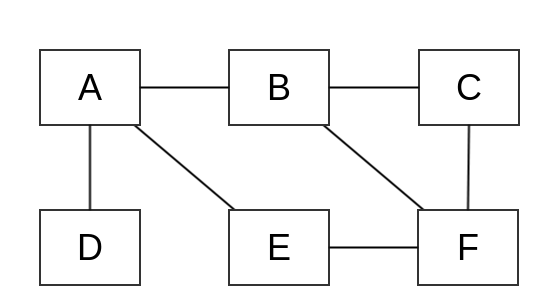
\includegraphics[width=0.45\linewidth]{Afbeeldingen/reversal.png}\end{center}
	\caption{Voorbeeld link reversal.}
	\label{fig:reversal}
\end{figure} 

Om dit beter uit te leggen wordt  \autoref{fig:reversal} gebruikt.
In de meeste gevallen wanneer A een bericht naar C wil sturen gaat hij zoeken naar een pad. 
Dit doet A door aan B en D  en E te vragen of zij C kennen wat vervolgens een heel netwerk zou doorlopen.
In elke bericht wordt de stap van route opgeslagen waardoor in het voorbeeld C uiteindelijk een drie berichten zou krijgen namelijk A-B-C, A-B-F-C en A-E-F-C. Deze stuurt C vervolgens weer terug waarop A kan bepalen welke route hij wil nemen waarbij A-B-C aannemelijk is aangezien dit de kortste route is. 

Bij link reversal werkt dit dus andersom \cite{Vainio_linkreversal}.
Hier maakt A bekend dat hij een route wil opbouwen naar C op dezelfde wijze als hierboven alleen begint C nu met het bouwen van een route. 
A zal dus uiteindelijk drie routes ontvangen C-B-A, C-F-B-A en C-F-E-A.

Op zich lijkt dit niet zo veel anders dan wat er normaal gebeurd maar dat is waar het LMR protocol komt kijken.
Na het versturen van een bericht naar C zijn er namelijk routes opgeslagen bij de punten te zien in \autoref{fig:reversallmr}

\begin{figure}[H]
	\begin{center}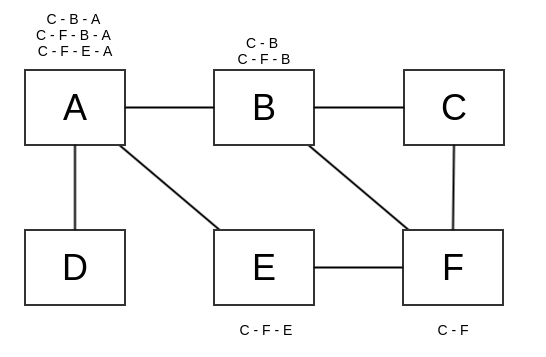
\includegraphics[width=0.5\linewidth]{Afbeeldingen/reversal-table.png}\end{center}
	\caption{Voorbeeld LMR na het versturen van een bericht.}
	\label{fig:reversallmr}
\end{figure} 

Nu op het moment dat A een bericht naar C wil sturen weet hij op basis van de informatie die hij heeft dat hij het bericht moet versturen naar B om het bij C terecht te laten komen.
Stel dat de verbinding B - C wegvalt dan weet B dat als hij het bericht aan F geeft dat het bericht nog steeds aan zal komen bij C.
Dit houdt dus is dat wanneer de verbinding B - C weg is dat A dit niet hoeft te weten want een bericht kan nog steeds succesvol verzonden worden via B.

Er hoeven dus alleen berichten verstuurd te worden over verloren verbindingen op het moment dat alle wegen verloren zijn.
In het geval van een dronenetwerk waar punten vaak veranderen zal dit aanzienlijk schelen in de hoeveelheid berichten die rondgestuurd zullen worden.

\subsection{Eigen implementatie idee voor de techniek}

Wat opvalt in de LMR techniek is dat er routes worden opgeslagen naar nodes toe waarop de richtingen worden bepaald.
De routes worden opgeslagen terwijl er alleen maar interesse is in de eerste stap van de route. 
In het voorbeeld van \autoref{fig:reversallmr} slaat A bijvoorbeeld route C-B-A en C-F-B-A op. 
Beiden geven het zelfde effect bij het zoeken voor een een route naar C, het bericht moet aan B gegeven worden.

Het idee, om ruimte te besparen, is om twee soorten tabellen bij te houden.
Een tabel van direct aangesloten punten waarbij elke aangesloten punt ook een eigen tabel heeft met punten waar deze directe buur mee kan communiceren.
In het bovenstaande voorbeeld zou dit betekenen dat A alleen hoeft te weten dat hij via B met C en F kan communiceren.
Dit bespaart ruimte in het opslaan van routes maar ook in de grootte van berichten. Nu hoeven er immers geen routes meer rondgestuurd te worden, maar alleen notificaties van nieuwe verbindingen.

Om te laten zien hoe deze implementatie zich vertaald naar een praktisch voorbeeld van een netwerk met een gateway en routers is er een extra afbeelding gemaakt te zien in \autoref{fig:routeringstabel}.

\begin{figure}[H]
	\begin{center}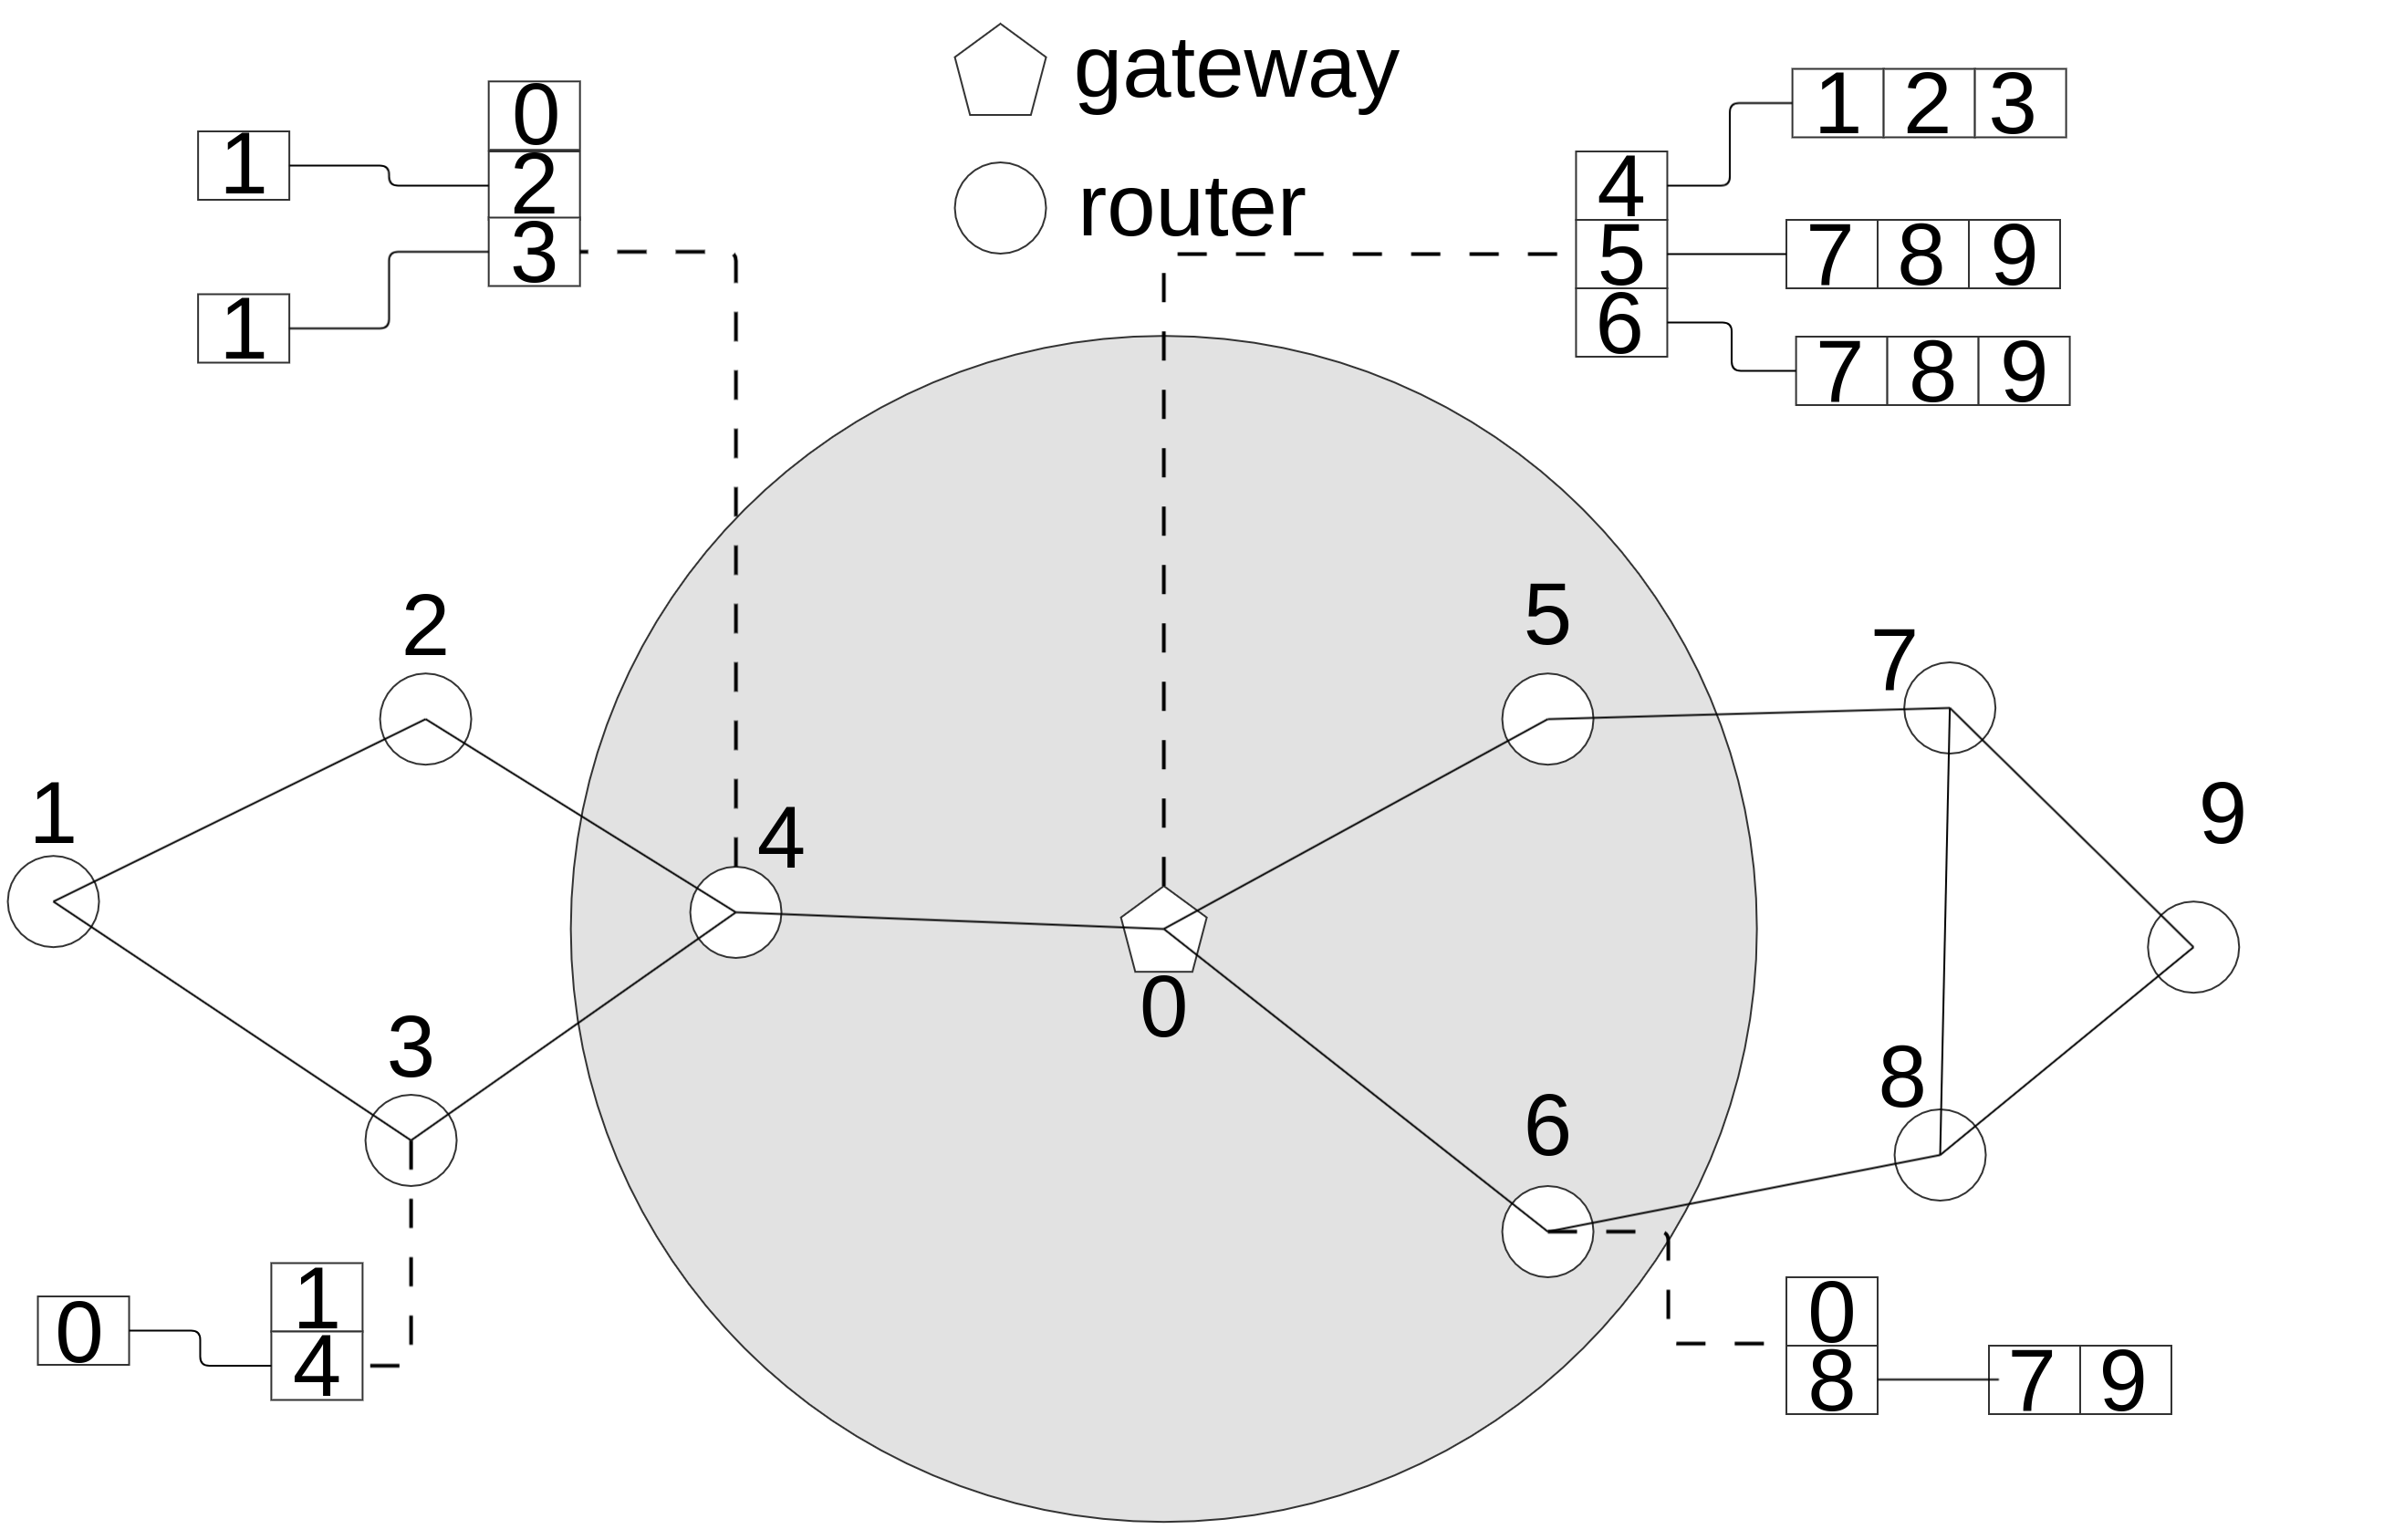
\includegraphics[width=0.6\linewidth]{Afbeeldingen/uitlegtabel.png}\end{center}
	\caption{Toelichting routeringstabel.}
	\label{fig:routeringstabel}
\end{figure}

In \autoref{fig:routeringstabel} wordt geïllustreerd hoe de routeringstabellen van een gateway en verschillende routers er uitzien.
Een nadeel van de huidige implementatie is dat er geen rekening wordt gehouden met het kortste pad door het netwerk.
Als in \autoref{fig:routeringstabel} bijvoorbeeld de gateway een bericht wil versturen naar router nummer 8 zal dit gebeuren via de weg 0-5-7-8 in plaats van de kortste weg 0-6-8.
Dit komt omdat er eerst gekeken wordt of het bericht voor een direct aangesloten punt is.
Wanneer dat niet zo is worden de tabellen van de indirecte punten nagelopen. 
De tabellen zijn gesorteerd op numerieke volgorde.
Wanneer het algoritme de tabellen van externe punten nazoekt zal de tabel van punt 5 als eerste een routepunt geven.

\subsection{Netwerk ondersteunen met heartbeats}

Een wens van Alten is dat het netwerk snel is en ook snel achter verloren verbindingen komt. 
De huidige implementatie van LMR zal dit beiden niet zijn om twee redenen.
LMR is event driven waardoor het alleen achter verloren verbindingen zal komen op het moment dat er een bericht geen route weet te vinden tot een punt in het netwerk.
Daarnaast worden routes pas opgebouwd op het moment dat er een bericht over het netwerk verstuurd wordt.
Tenslotte hebben de routers een belang bij de kennis of ze verbinding hebben met een gateway in het netwerk van Alten, omdat dit hun verbindingspunt is met de buitenwereld.

Een oplossing voor al deze problemen is het implementeren van een functie in elke router dat periodiek moet proberen een bericht naar een gateway te sturen. Als response op deze heartbeat zal de router ook weer een heartbeat terug moeten sturen.
Deze oplossing zou zorgen dat het netwerk zijn routes blijft onderhouden door ze periodiek te controleren.
Het zou ook zorgen dat een gateway altijd bekend is met alle mogelijke routes omdat hij weet welke node er in elke richting beschikbaar is. Bij het versturen van een bericht hoeft er dus niet eerst een route opgebouwd te worden.
Tenslotte zou het sturen van een response de router meteen bewust maken of er een verbinding bestaat naar een gateway.

\subsection{Conclusie}  

Het veranderen van de LMR door er heartbeat aan toe te voegen maakt de techniek deels proactief. 
Zoals al eerder beschreven is een routeringstechniek die deels proactief is en deels reactief een hybride techniek.
Vandaar dat deze techniek onder naam zal vallen hybride lightweight mobile routing (H-LMR).
In de huidige implementatie of die van de originele LMR wordt geen rekening gehouden met het kortste pad.
Op het moment dat dit wel wenselijk wordt kunnen de heartbeat berichten uit het netwerk gebruikt worden.
Deze zijn inzetbaar om het aantal hops te tellen die een bericht heeft ondergaan om zo te registreren hoever een node per punt verwijderd is.
Een keerzijde zou zijn dat er wel weer extra rekenkracht vereist wordt voor het zoeken van een pad.

\section{Een stap terug voor netwerkherstel}\label{sec:drone-aansturing-een-stap-terug-voor-netwerkherstel}

Elke netwerkmodule zit aangesloten op een drone en heeft de mogelijkheid om deze aan te sturen.
Alten wil gebruik maken van deze combinatie om zo het herstellend vermogen te vergroten van het netwerk.
In de stuk wordt een uitwerking beschreven waar netwerkmodules zich een stap terug verplaatsen in het netwerk om zo een poging te doen een verloren verbinding te herstellen.

\subsection{Een enkele drone die verloren is}\label{sec:een-enkele-drone-die-verloren-is}
\autoref{fig:enkel_goed} laat een lus van drones zien die met elkaar verbonden zijn en op die wijze een netwerk verspreiden. Deze situatie wordt gebruikt om het gedrag te omschrijven die uitgevoerd moet worden door de drones op het moment dat er een verbinding verloren gaat. 
\begin{figure}[H]
	\begin{center}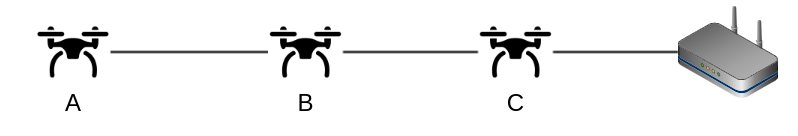
\includegraphics[width=.85\linewidth]{Afbeeldingen/droneopstelling_enkel_goed.png}\end{center}
	\caption{Situatie waar drie drones met elkaar in verbinding staan.}
	\label{fig:enkel_goed}
\end{figure} 

\paragraph{Verlies van een enkel punt}
Op het moment dat er een enkel punt wegvalt waardoor er een drone alleen overblijft moet hij zich verplaatsen naar het weggevallen punt. Dit wordt geïllustreerd in \autoref{fig:enkel_B_kapot} waar B uitvalt waardoor A zich zal herpositioneren op de positie van B. 
\begin{figure}[H]
	\begin{center}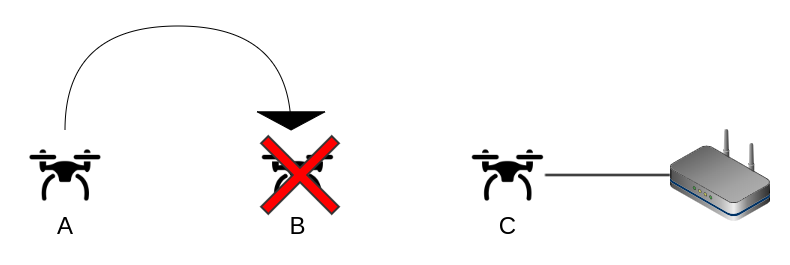
\includegraphics[width=.85\linewidth]{Afbeeldingen/droneopstelling_enkel_B_kapot.png}\end{center}
	\caption{Situatie waar drone B is uitgevallen.}
	\label{fig:enkel_B_kapot}
\end{figure}

\paragraph{Verlies van een twee punten}
Wanneer er twee punten wegvallen zoals te zien in \autoref{fig:enkel_B_C_kapot} wordt er verwacht van de drone dat hij eerst naar punt B vliegt.
Zodra de drone op punt B is gaat de netwerkmodule opnieuw zoeken naar een nieuwe verbinding.
In deze situatie zal de netwerkmodule geen nieuw punt vinden waardoor de volgende stap is dat de drone terugkeert naar de gateway.  
\begin{figure}[H]
	\begin{center}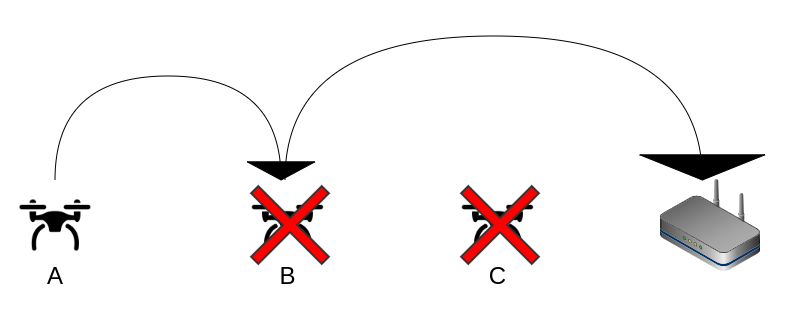
\includegraphics[width=1\linewidth]{Afbeeldingen/droneopstelling_enkel_B_en_C_kapot.png}\end{center}
	\caption{Situatie waar drone B en C zijn uitgevallen.}
	\label{fig:enkel_B_C_kapot}
\end{figure}
 
\subsection{Een groep drones die verloren is}\label{sec:een-groep-drones-die-verloren-is}

Wanneer er een groep verloren gaat komt er meer kijken bij het herverdelen van de drones.
Het zou namelijk geen zin hebben om alle drones te verplaatsen naar een stap terug in het netwerk op het moment dat deze plek hetzelfde is voor meerdere drones.
Om de herverdeling die uitgevoerd wordt toe te lichten wordt er vanuit gegaan dat de drones verdeelt zijn zoals te zien in \autoref{fig:groep_goed}.

\begin{figure}[H]
	\begin{center}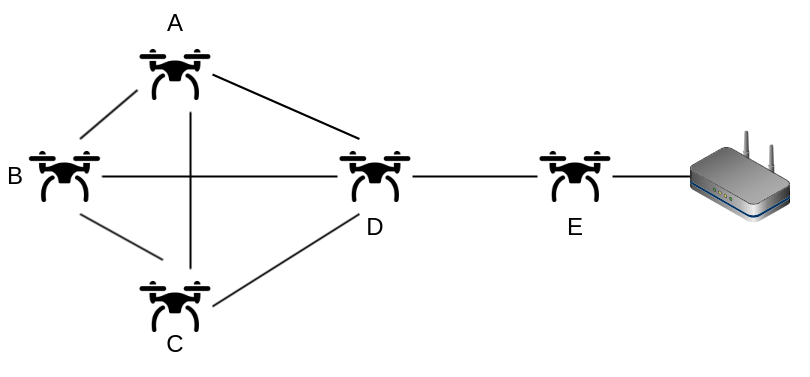
\includegraphics[width=1\linewidth]{Afbeeldingen/droneopstelling_Groep_goed.png}\end{center}
	\caption{Situatie waar drie drones met elkaar in verbinding staan.}
	\label{fig:groep_goed}
\end{figure} 

\paragraph{Uitval van een enkele drone die het directe aanknooppunt is voor de groep}
De eerste situatie die wordt toegelicht is wanneer er een drone uitvalt die de laatste drone is die de groep met de rest van het netwerk verbind.
Deze situatie wordt geschetst in \autoref{fig:groep_B_kapot}. 
In dit figuur valt punt D uit waardoor punt A, B, en C geen verbinding meer hebben.
Vervolgens moeten deze drie punten met elkaar communiceren wie er gaat bewegen naar punt D.
Zij zullen alle drie de afstand communiceren die zij hebben tot de locatie van de gateway. 
Vervolgens zal de drone de die grootste afstand heeft, in dit geval B, zich verplaatsen naar locatie D.
Als de drone op locatie D staat kan hij een verbinding leggen met drone E waardoor A en C ook via hem weer verbinding krijgen.

\begin{figure}[H]
	\begin{center}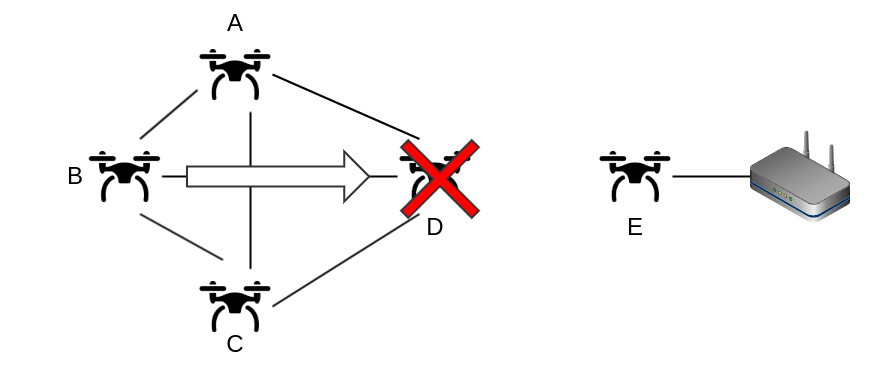
\includegraphics[width=.8\linewidth]{Afbeeldingen/droneopstelling_Groep_een_kapot.png}\end{center}
	\caption{Situatie waar drone D is uitgevallen.}
	\label{fig:groep_B_kapot}
\end{figure}

\paragraph{Uitval van een enkele drone die het indirecte aanknooppunt is voor de groep}
Als punt E uitvalt zoals te zien in \autoref{fig:groep_E_kapot} zou alleen een berekening wie het verste van de gateway afstaat het effect hebben dat drone B zich moet verplaatsen naar de plek van drone D.
Dit terwijl drone D nog gewoon werkt.
Daarom zal er in de onderhandeling over wie zich moet verplaatsten worden meegenomen of er al een andere drone op de plek staat.
Als dit zo is sluit de drone zichzelf buiten van de onderhandeling.
In de situatie waar drone E uitvalt zal dit dus betekenen dat drone D zich naar de positie van E verplaatst.
Vervolgens zullen de drones A-B-C alsnog geen verbinding hebben waardoor er opnieuw onderhandeld moet worden. 
Het resultaat moet dan zijn dat B zich verplaatst naar de oude positie van D.  

\begin{figure}[H]
	\begin{center}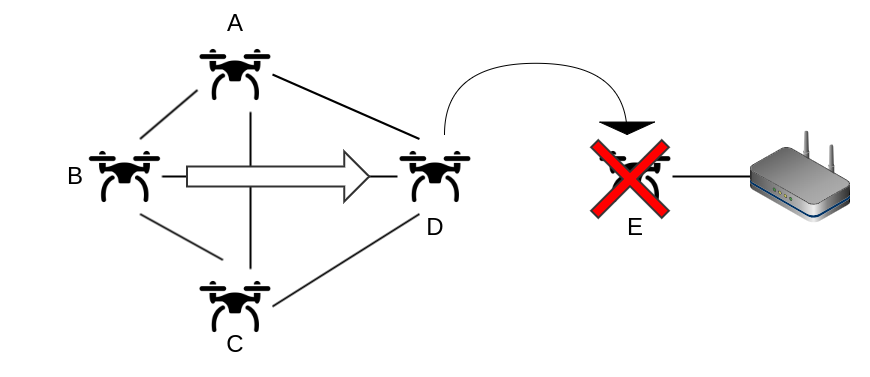
\includegraphics[width=.8\linewidth]{Afbeeldingen/droneopstelling_GroepXL_een_kapot.png}\end{center}
	\caption{Situatie waar drone E is uitgevallen.}
	\label{fig:groep_E_kapot}
\end{figure}

\paragraph{Uitval van twee drones die het aankooppunt zijn voor de groep}
Op het moment dat allebei de punten D en E uitvallen zullen de drones uiteindelijk allemaal terugkeren naar de gateway. 
Het effect zal zijn dat punt A, B en C zich eerste naar punt D zullen verplaatsen en vervolgens terugkeren naar de gateway.    
\begin{figure}[H]
	\begin{center}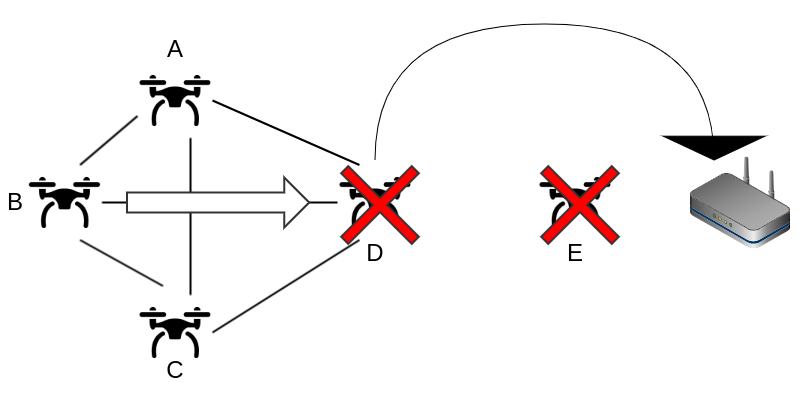
\includegraphics[width=.85\linewidth]{Afbeeldingen/droneopstelling_Groep_meer_kapot.png}\end{center}
	\caption{Situatie waar drone B en C zijn uitgevallen.}
	\label{fig:groep_B_C_kapot}
\end{figure}


\subsection{Conclusie}

Het protocol om de drone een stap terug te laten zetten in het netwerk is een zwak protocol die wel gemakkelijk te implementeren is.
Het is bedacht met het idee om te laten zien dat er potentie zit in het gebruiken van drones voor het bevorderen van het zelfherstellend vermogen van netwerken.
De implementatie zal geen optimale verdeling bevorderen en geeft het netwerk alleen maar een kans om zich te herstellen op het moment dat er een enkele drone uitvalt.
Desalniettemin toont het idee wel aan dat drones toepasbaar kunnen zijn voor het zelfherstellend vermogen.


\chapter{Experimenten}
\label{experimenten}


\section[Hybride-LMR]{Hybride lightweight mobile routing protocol}

Om het aangepaste protocol van \autoref{sec:hybride-lightweight-mobile-routing} te testen zal er gebruik gemaakt worden van de simulatie.
Uit het protocol kunnen de volgende stukken pseudo code geleerd worden.

\subsection{Ontvangen van een bericht}

Met het H-LMR protocol leert een netwerkpunt van elk bericht die langskomt over andere zenders in het netwerk.
Hierin maakt het niet uit of het bericht bestemd is voor het ontvangende punt of dat het doorgestuurd moet worden. 

\begin{lstlisting}

recieveMessage(message){
	message[destination] == this->address ? processMessage(message) : forwardMessage(message);
	
	add the sender of the message to the direct connections
	if(message[sender] != message[creator])
	{
	add the creator of the message to the indirect connection table of the sender
	}
}

\end{lstlisting}

\subsection{Doorsturen van een bericht}

Het H-LMR stelt dat wanneer een bericht aankomt die doorgestuurd moet worden dat de ontvanger zelf zoekt wie de volgende stap neemt.
Pas als er geen volgende stap mogelijk is mag de node een informatie bericht versturen over een verloren verbinding.

\begin{lstlisting}

forwardMessage(message){
int direction = getDirection(message[destination]);
if (direction == NOT_FOUND || direction == message[sender])
	{
	inform the sender of the message about a invalid path
	return;
	}
else 
	{
	Forward the message to the found direction
	}	
}

\end{lstlisting}

\subsection{Test met zes routers en een gateway}

Om het protocol te testen wordt de testopstelling gebruikt getoond in \autoref{fig:testopstelling-gateway-zes-routers}.

\begin{figure}[H]
	\begin{center}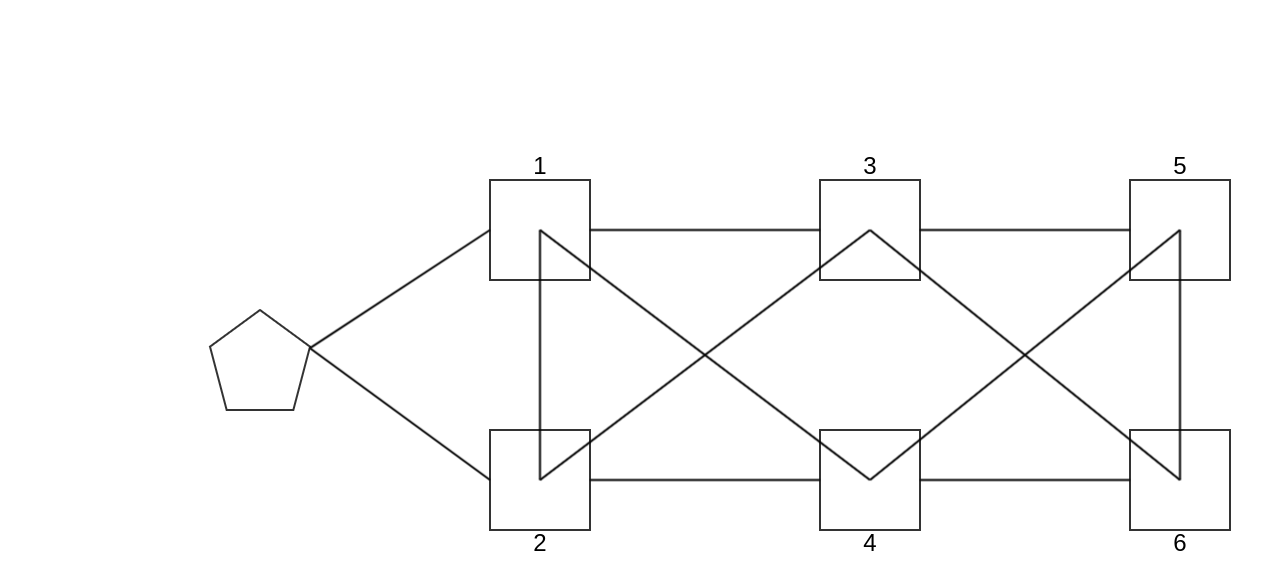
\includegraphics[width=1\linewidth]{Afbeeldingen/testopstelling1.png}\end{center}
	\caption{Testopstelling met links een gateway waarna zes routers volgen.}
	\label{fig:testopstelling-gateway-zes-routers}
\end{figure}

In deze opstelling is de begin positie het netwerk zoals die getoond wordt op de afbeelding.
In de applicatie ziet dit er als volgt uit.


\begin{figure}[H]
	\begin{center}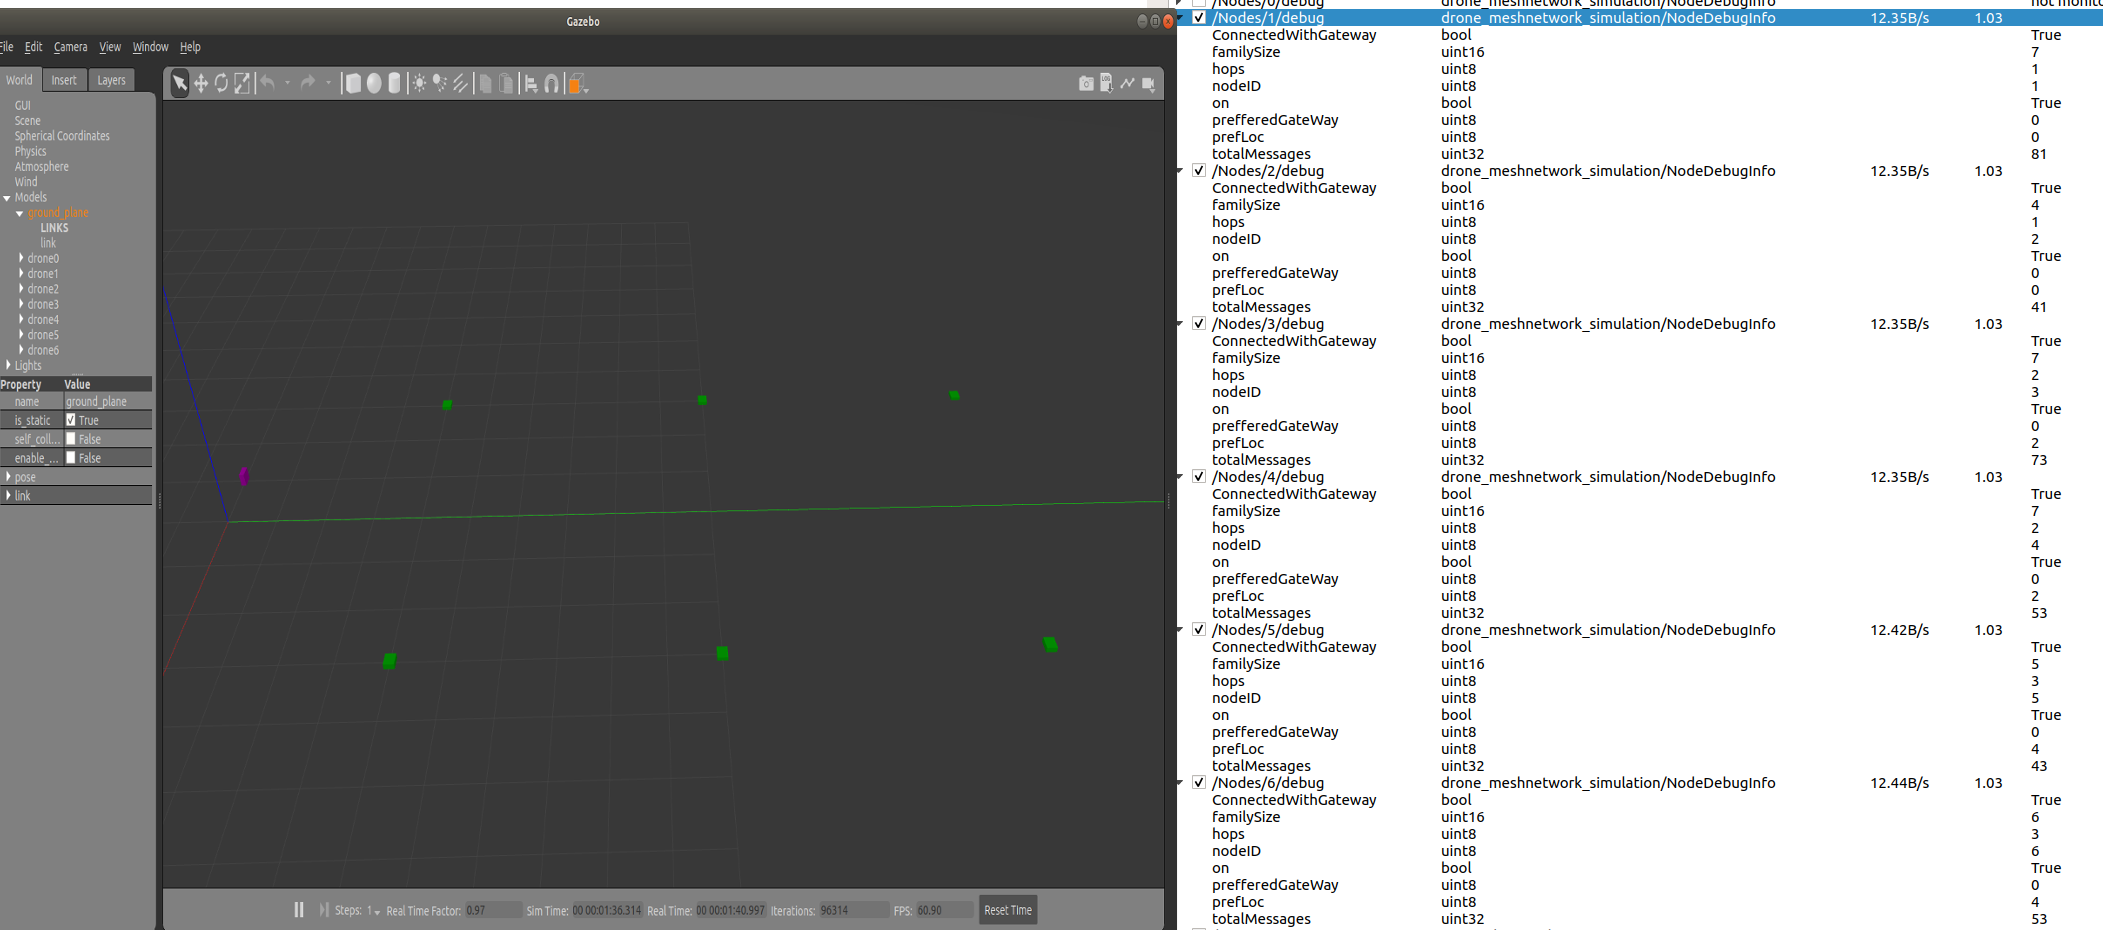
\includegraphics[width=1\linewidth]{Afbeeldingen/testopstellingmetzes_debug_info_fusion.png}\end{center}
	\caption{Applicatie Gazebo waar zes routers en een gateway getoond worden samen met debug informatie.}
	\label{fig:applicatie-testopstelling-gateway-zes-routers}
\end{figure}  

In \autoref{fig:applicatie-testopstelling-gateway-zes-routers} is rechts debug informatie zichtbaar.
De eerste waarde van elke router (ConnectedWithGateway) laat zien of verbinding is met een gateway.
In het huidige geval heeft dus elke router verbinding met een gateway.

\paragraph{Uitval van drone 3}

\begin{figure}[H]
	\begin{center}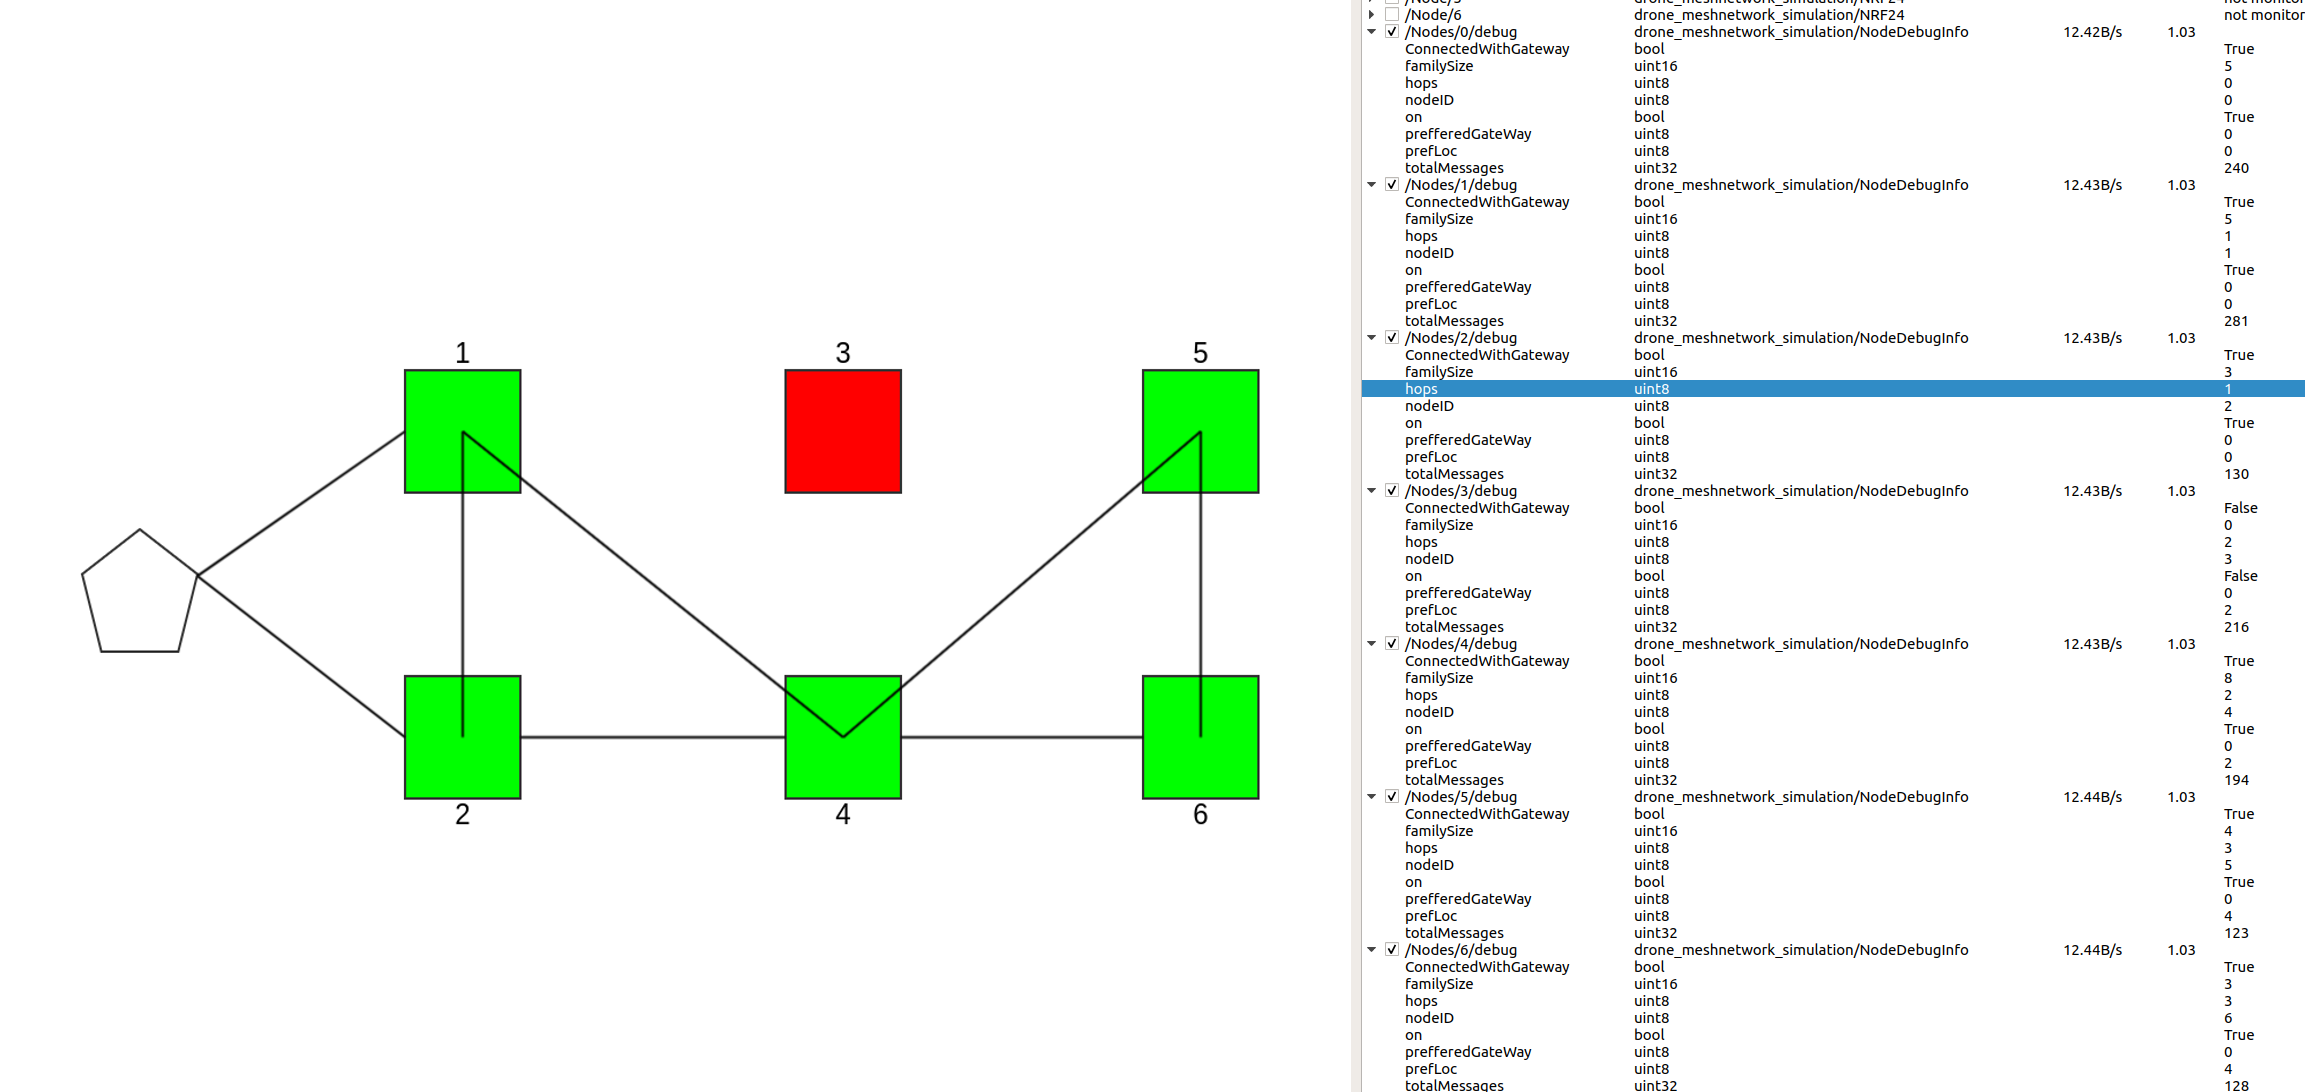
\includegraphics[width=\linewidth]{Afbeeldingen/testopstellingmetzes_debug_info_drie_is_uit.png}\end{center}
	\caption{Debug informatie van testopstelling waar punt drie is uitgezet.}
	\label{fig:applicatie-testopstelling-gateway-zes-routers-drie-is-uit}
\end{figure}   
Op het moment dat punt 3 wordt uitgezet blijven punt 5 en 6 verbonden met de gateway zoals verwacht.
In de debug informatie wordt ook een variabel getoond met de naam familySize. 
Deze variabele is een som van alle tabellen in een node.  
Wat opvalt na het uitzetten van punt 3 is dat punt 5 zijn familySize verkleint van 7 naar 4. 
Dit houdt dus in dat punt 5 drie routes had opgebouwd via punt 3 waarvan één route natuurlijk 5-3 was.
De andere routes waren naar alle waarschijnlijkheid 5-3-1 en 5-3-0.

\paragraph{Uitval van drone 3 en 6}
\begin{figure}[H]
	\begin{center}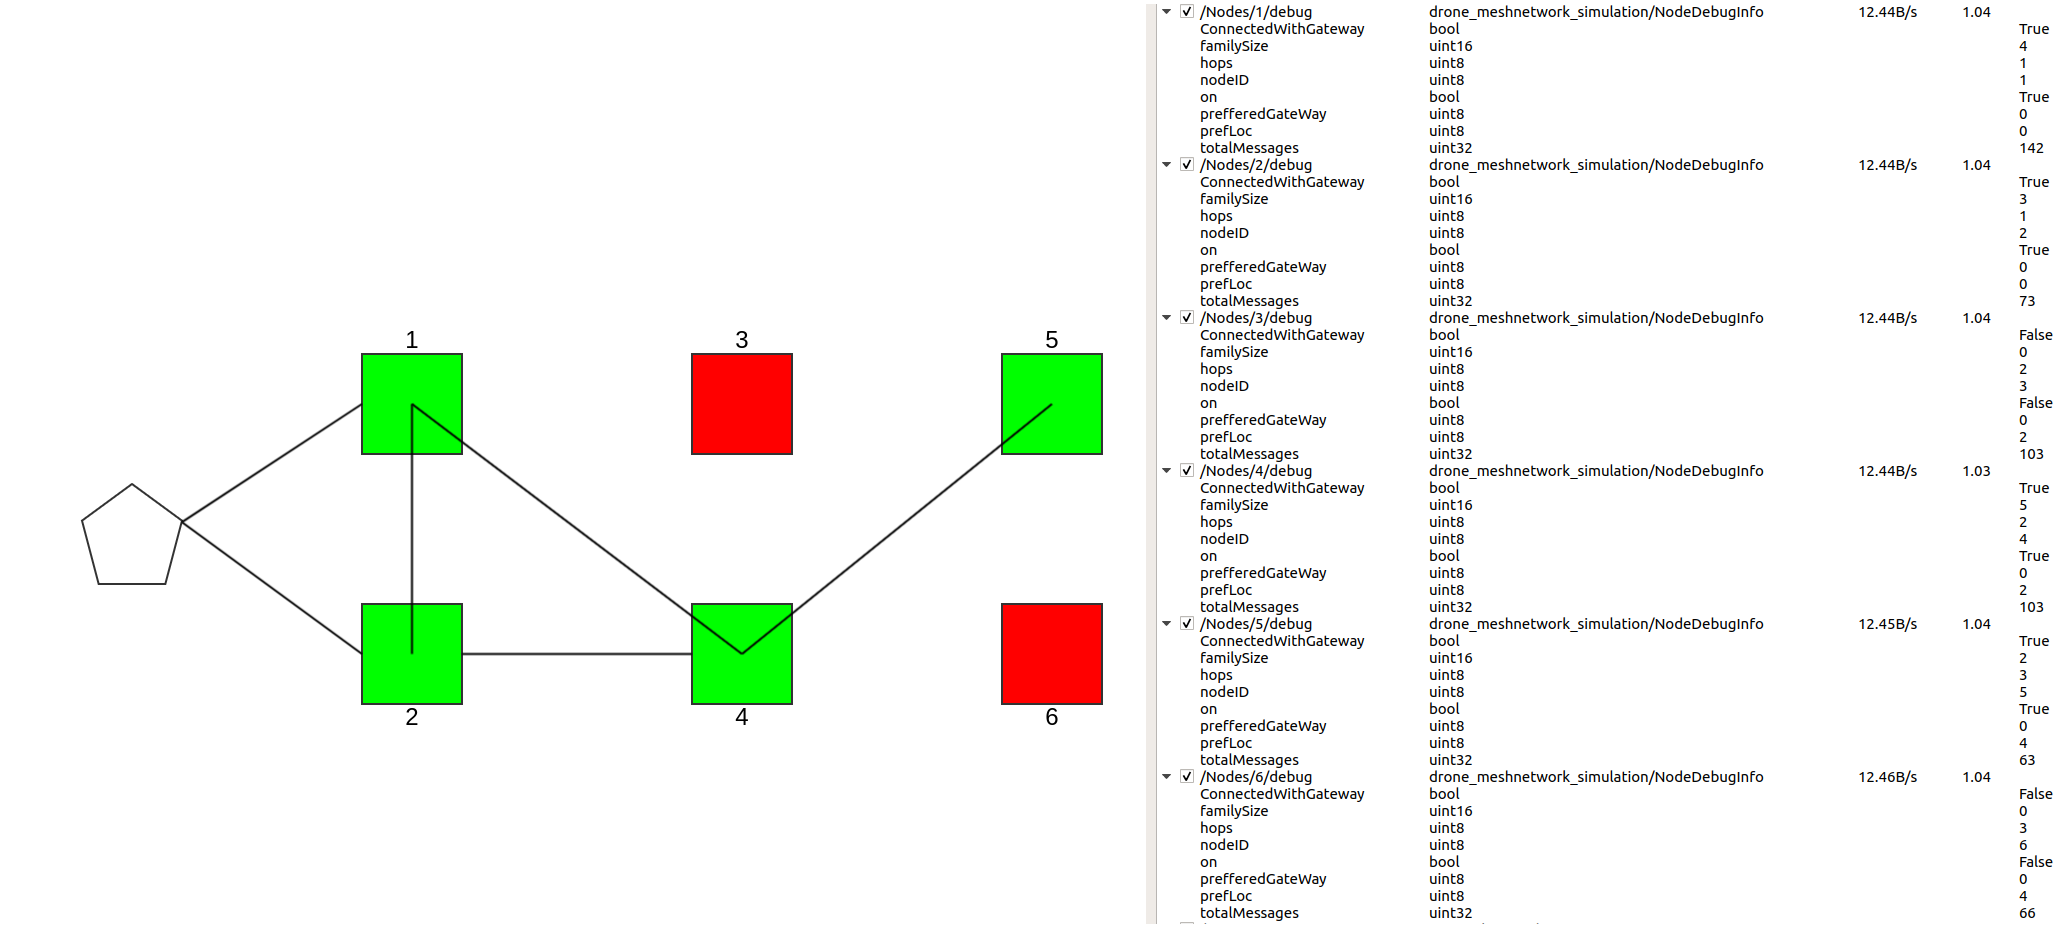
\includegraphics[width=\linewidth]{Afbeeldingen/testopstelling1_drie_en_zes_is_uit.png}\end{center}
	\caption{Debug informatie van testopstelling waar punt drie en zes is uitgezet.}
	\label{fig:applicatie-testopstelling-gateway-zes-routers-drie-en-zes-is-uit}
\end{figure}

\autoref{fig:applicatie-testopstelling-gateway-zes-routers-drie-en-zes-is-uit} laat zien hoe het netwerk zich gedraagt als punt zes ook wordt uitgezet.
Zoals verwacht heeft punt 5 nog steeds een verbinding met een gateway.
In de informatie is te zien dat punt 5 nog maar bewust is van twee routes. 
Er kan met zekerheid gezet worden dat dit route 5-4 en 5-4-0 zullen zijn.

\paragraph{Uitval van drone 3, 4 en 6}
\begin{figure}[H]
	\begin{center}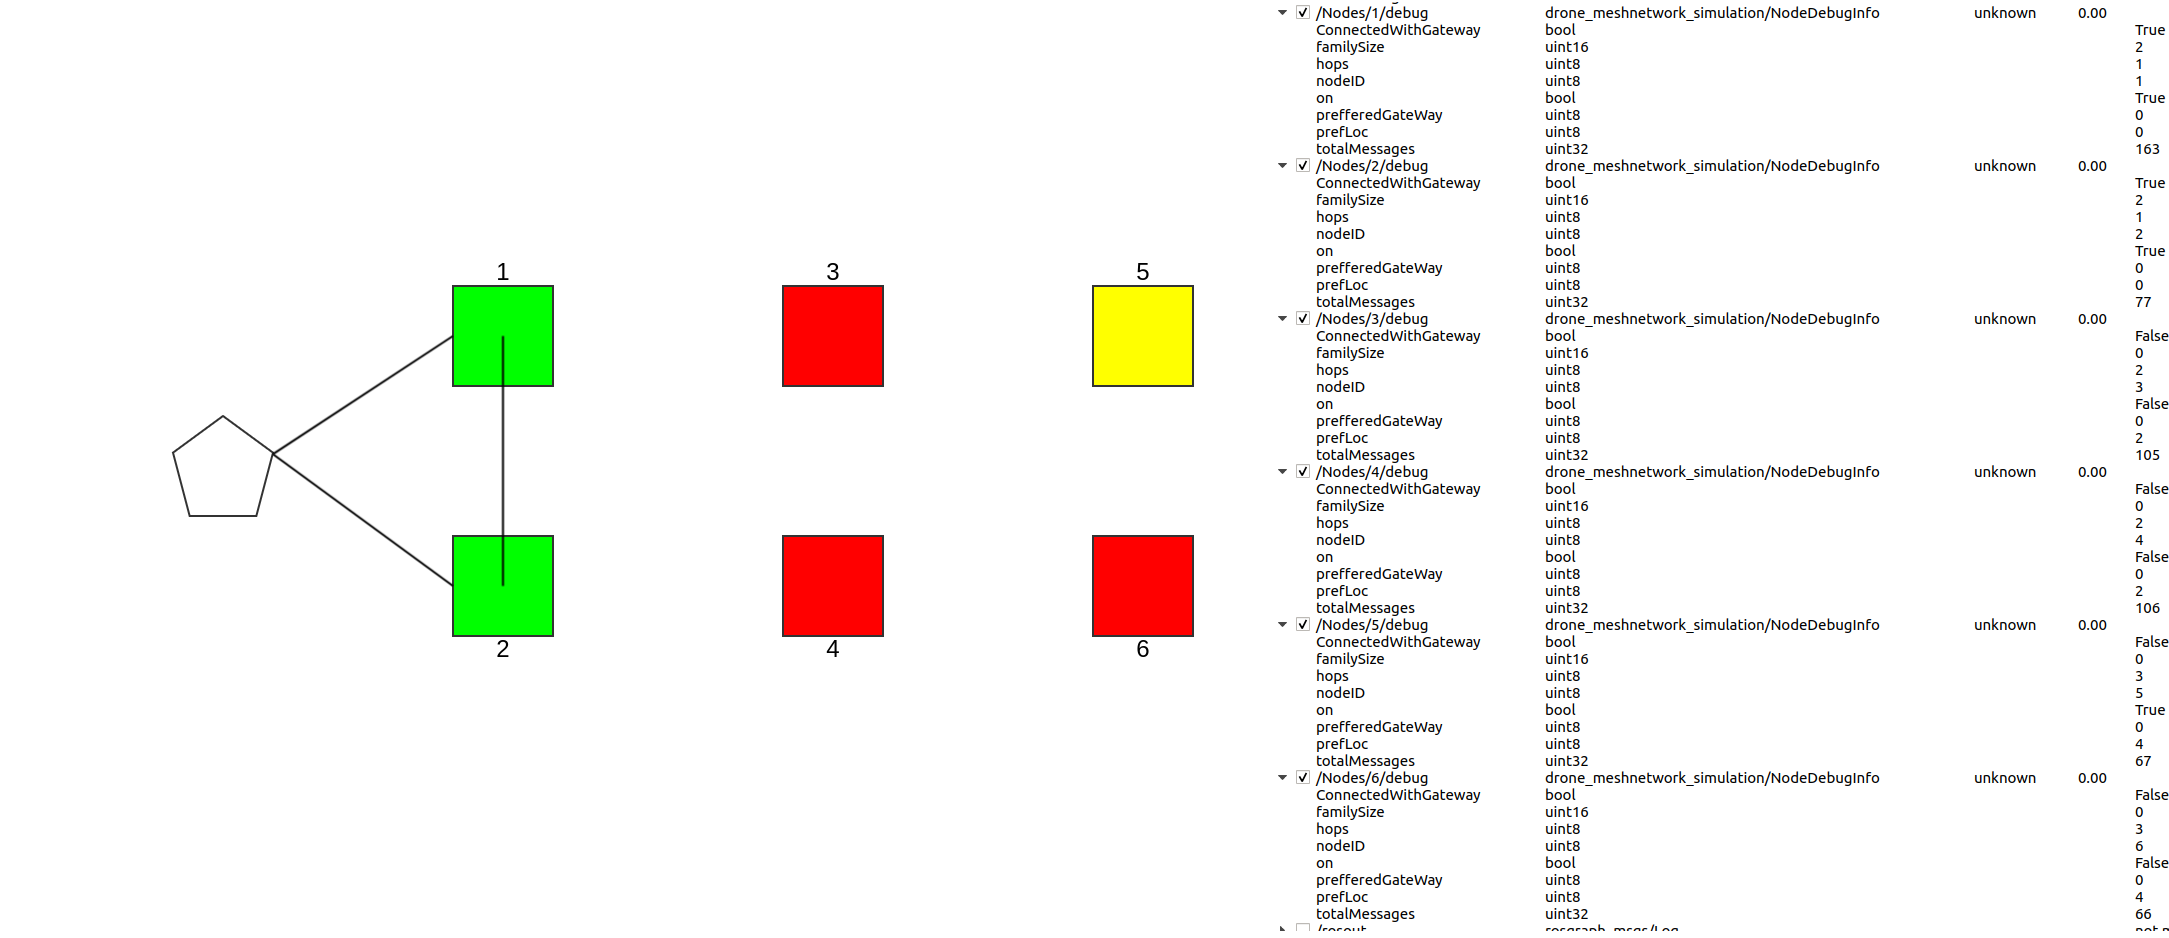
\includegraphics[width=\linewidth]{Afbeeldingen/testopstellingmetzes_drie-vier-zes-uit.png}\end{center}
	\caption{Debug informatie van testopstelling waar punt drie, vier en zes is uitgezet.}
	\label{fig:applicatie-testopstelling-gateway-zes-routers-drie-vier-en-zes-is-uit}
\end{figure}

In deze opstelling zijn punten 3, 4 en 6 uitgezet. In de debug informatie is te zien dat punt 5 zijn verbinding verloren is.
Zowel punt 1 en punt 2 geven aan twee routes te kennen.
Dit is zoals verwacht.

\begin{figure}[H]
	\begin{center}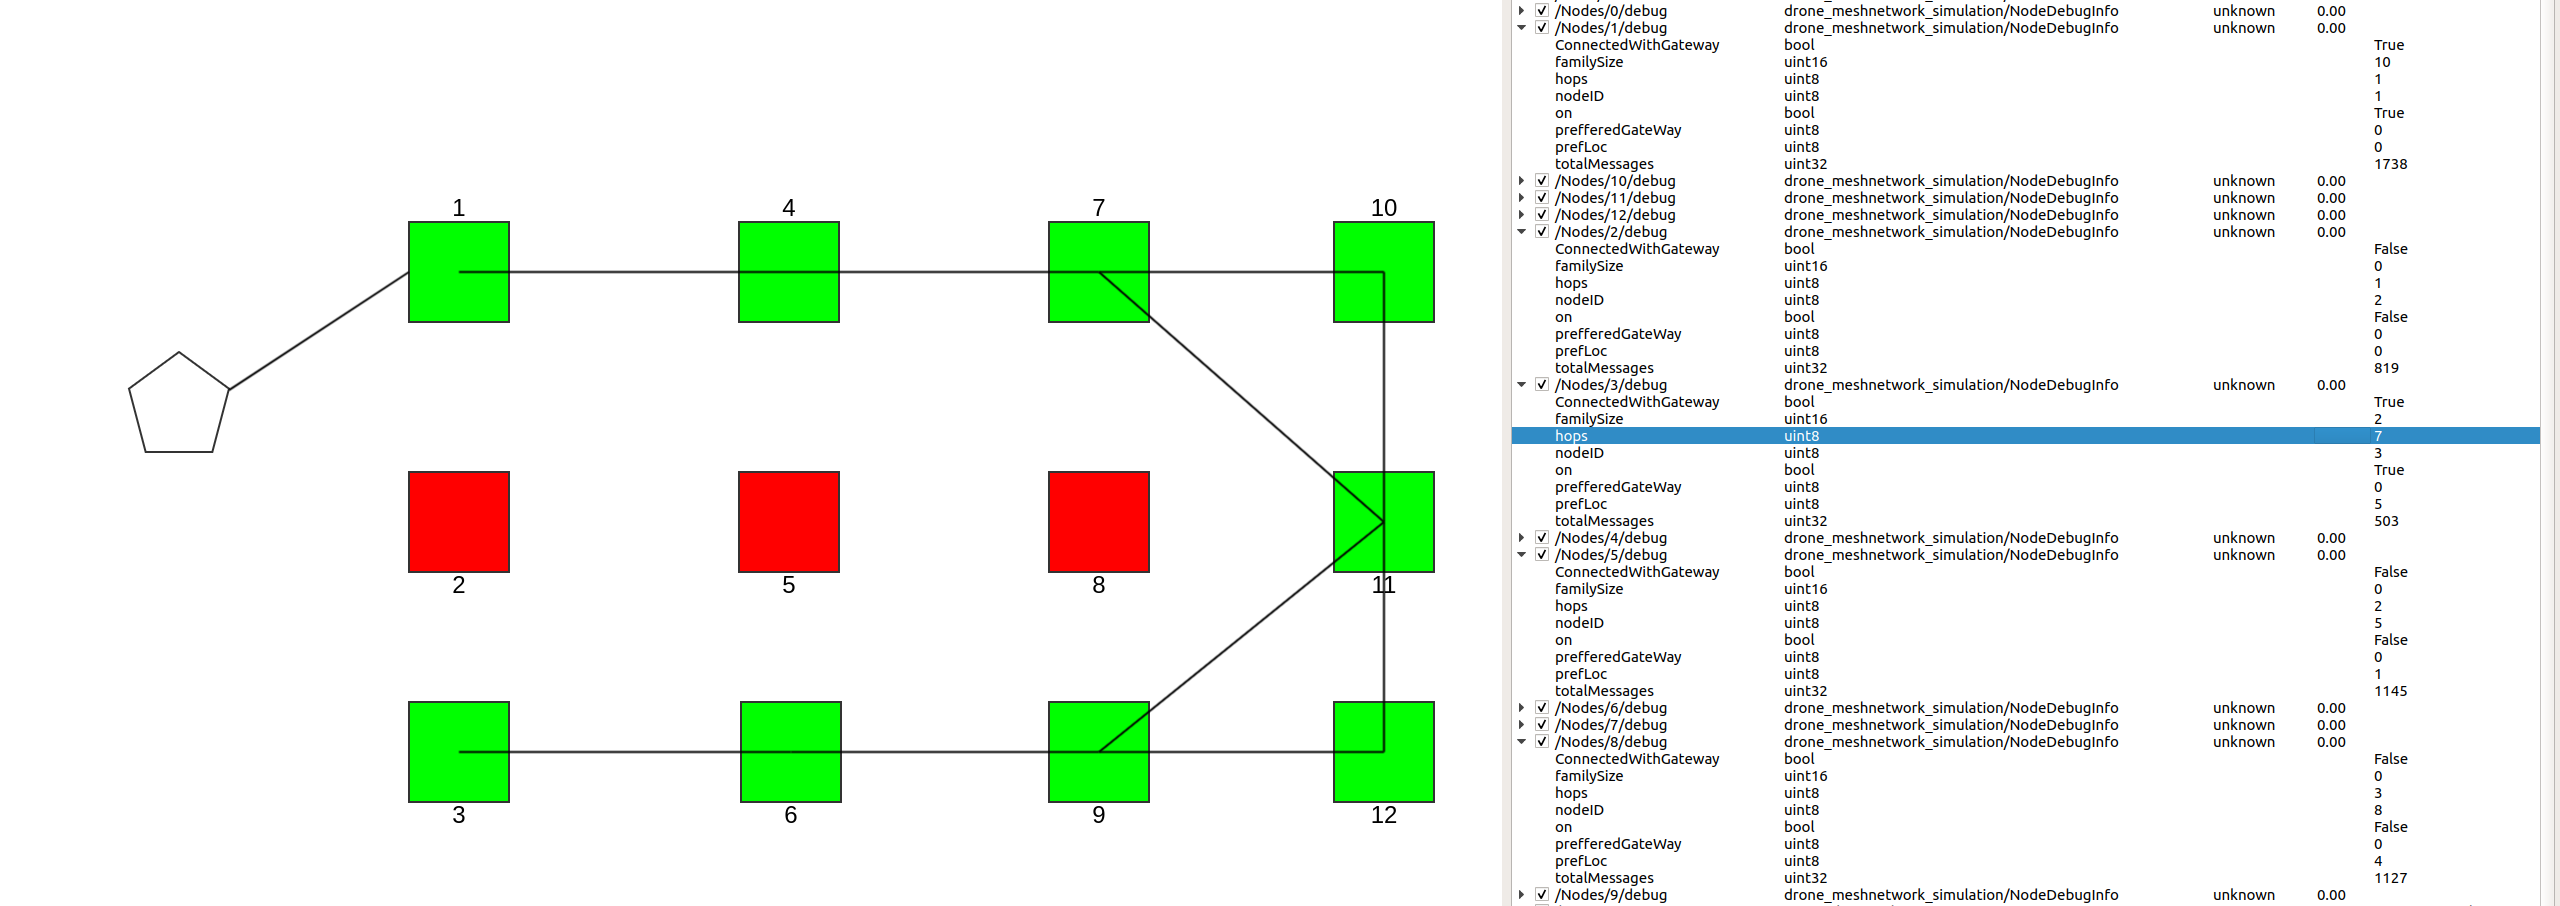
\includegraphics[width=\linewidth]{Afbeeldingen/testopstelling2_met_twaalf_drie_routers_uit.png}\end{center}
	\caption{Debug informatie van testopstelling met 12 routers waar punt twee, vijf en acht is uitgezet.}
	\label{fig:applicatie-testopstelling-gateway-twaalf-routers}
\end{figure}

Als laatste opstelling is een opstelling van twaalf routers gebruikt.
Hier zijn routers 2, 5, en 8 uitgezet om router nummer 3 te forceren via een grote omweg te communiceren naar de gateway.
In de debug informatie is te zien dat hij hierin geslaagd is en dat er 7 hops nodig zijn voor de gateway om een route naar de router te vinden.
Dit betekend dat er de volgende route wordt gebruikt 0-1-4-7-11-9-6-3.

\subsection{Conclusie}

Het experiment waarin de aangepaste versie van LMR wordt getest bewijst dat de techniek bruikbaar is voor het dronenetwerk.
Er zijn genoeg scenario's getest om aan te tonen dat het netwerk zichzelf kan herstellen wanneer er een verbinding verloren is gegaan.

\section[Netwerkherstel door beweging  drone]{Is het mogelijk voor netwerkmodule om een netwerk te herstellen door het de mogelijkheid te geven zich vrij te bewegen?}
\label{experimenten:herstelnetwerk}

In \autoref{sec:drone-aansturing-een-stap-terug-voor-netwerkherstel} wordt een voorstel gedaan voor het herstellen van het netwerk door drones een stap terug te laten nemen in het netwerk. Eerst wordt er kort toegelicht wat er toegevoegd moet worden aan de modules om dit mogelijk te maken. Vervolgens worden de bedachte scenario's getest.Tenslotte zal in de conclusie een oordeel gegeven worden over de effectiviteit van het voorstel.

\subsection{Aanpassingen voor de software}
In het voorstel wordt gesteld dat de drone terug moet vliegen naar het punt in het netwerk die een stap dichterbij de gateway is.
Om dit te kunnen doen moet een drone wel weten waar dit is.
Hiervoor kunnen de onderhoud berichten gebruikt worden die al bestaan in het netwerk aangezien er toch alleen interesse is in de locatie van directe buren.
In pseudo code zou er dan het volgende ontstaan. 
\begin{lstlisting}
if(message[hops aways from gateway] < our hops away from gateway && not already used as location by this node)
{
	requestLocationOf(message[creator])
}
\end{lstlisting}

Een andere locatie die een router gebruikt in het protocol voor herstel is de locatie van de gateway. 

Het is daarom belangrijk dat de node altijd op de hoogte is van de locatie van een gateway.
Op het moment dat er een verbinding komt met een gateway moet een router dus zo snel mogelijk de locatie van deze gateway opvragen.

Verder moet er een aanpassing komen in de software voor een onderhandeling binnen een groep over wie er moet verplaatsen.
Dit zal gebeuren door gezamenlijk een tabel op te bouwen door de afstand uit te wisselen die elke router van een gateway verwijderd is.

\begin{table}[H]
	\centering
		\begin{tabular}{|
				>{\columncolor[HTML]{C0C0C0}}l |
				>{\columncolor[HTML]{FD6864}}l |
				>{\columncolor[HTML]{FD6864}}l |
				>{\columncolor[HTML]{67FD9A}}l |l|l|}
			\hline
			ID & 3 & 5 & 1 & 4 & 2 \\ \hline
			Afstand & -1 & -1 & 12 & 12 & 16 \\ \hline
		\end{tabular}%

	\caption{Het selecteren van een drone die zich moet verplaatsen.}
	\label{tab:afstandtabelverplaatsing}
\end{table}

In \autoref{tab:afstandtabelverplaatsing} wordt een voorbeeld gegeven van een tabel waar dit overleg gepleegd is. 
Drone 5 en 3 hebben in dit tabel aangegeven dat verplaatsen voor hun geen zin heeft door een waarde van -1 te sturen sluiten ze zichzelf buiten.
Door de tabel te sorteren, in dit geval van links naar rechts, kan elke drone kijken of hij het ID heeft van de eerste drone met een waarde boven 0. Als hij dit heeft wordt hij aangewezen om zich te verplaatsen.

\subsection{Test met een enkele drone die zijn verbinding verliest}

In \autoref{sec:een-enkele-drone-die-verloren-is} worden situaties besproken die een drone zou moeten ondernemen zodra hij zijn verbinding verliest. Het gaat hier om stappen die een drone moet ondernemen als hij zijn verbinding verloren is met elk mogelijk punt in de buurt.
Deze worden getest met een simulatie waar de drones gelijk aan de situatie zijn verdeeld zoals te zien in 	\autoref{fig:applicatie-testopstelling-drones-in-sim}.

\begin{figure}[H]
	\begin{center}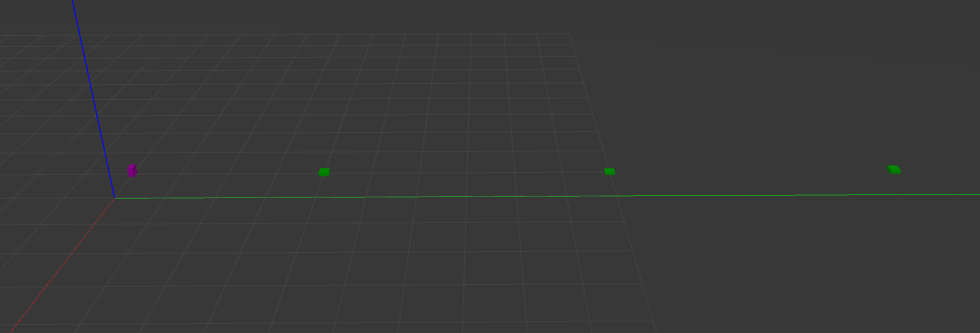
\includegraphics[width=\linewidth]{Afbeeldingen/droneopstelling_in_sim.png}\end{center}
	\caption{Drone verdeeld volgens de testopstelling in de simulatie.}
	\label{fig:applicatie-testopstelling-drones-in-sim}
\end{figure}
\paragraph{Test 1:} In de eerste test wordt de situatie nagebootst zoals deze wordt omschreven in \autoref{fig:enkel_B_kapot}.
Deze test is opgenomen en zichtbaar in bijlage \ref{sec:enkele-verloren-drone-situatie-1mp4}. 
Hier is te zien dat de oplossingsrichting voor een enkele drone die zijn verbinding verliest werkt voor het herstel.

\paragraph{Test 2:} In de tweede test wordt de situatie nagebootst zoals deze wordt omschreven in \autoref{fig:enkel_B_C_kapot}.
Deze test is opgenomen en zichtbaar in bijlage \ref{sec:enkele-verloren-drone-situatie-2mp4}.
In de video is te zien dat de drone het gedrag volgt zoals die in de oplossingsrichting omschreven is. 


\subsection{Test met een groep drones die hun verbinding verliest}
\autoref{sec:een-groep-drones-die-verloren-is} beschrijft hoe drones zich zouden moeten gedragen op het moment dat ze als groep verloren zijn.
Dit is geïmplementeerd in de software en wordt hier getest en kort omschreven.

\begin{figure}[H]
	\begin{center}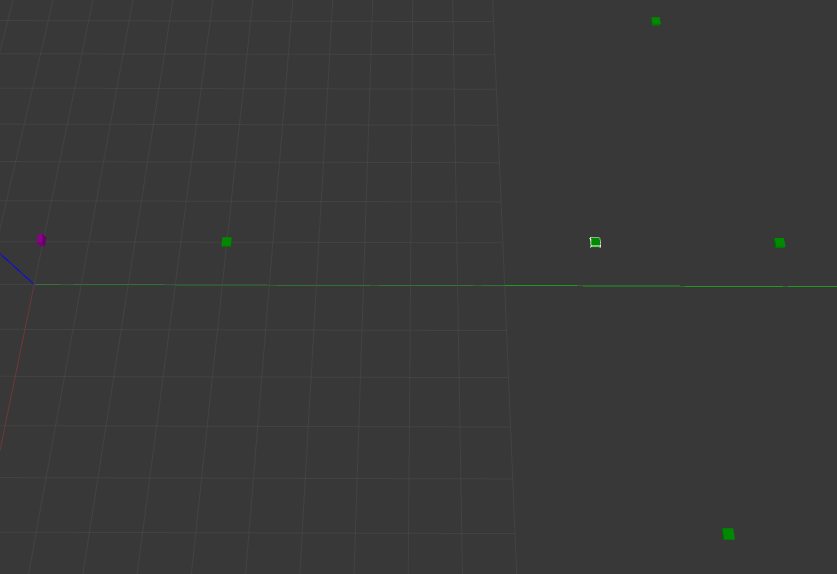
\includegraphics[width=.7\linewidth]{Afbeeldingen/testopstelling2_in_simulatie.png}\end{center}
	\caption{Drones verdeeld volgens de testopstelling in de simulatie.}
	\label{fig:applicatie-testopstelling-2-drones-in-sim}
\end{figure}


\paragraph{Test 1:} In de eerste test wordt de situatie nagebootst zoals deze wordt omschreven in \autoref{fig:groep_B_kapot}.
Deze test is opgenomen en zichtbaar in bijlage \ref{sec:groep-verloren-drones-situatie-1mp4}. 
In de video is te zien dat de drone die de grootste afstand tot de gateway verwijderd is zich verplaatst naar de positie van de uitgevallen drone. Vervolgens komt deze terug in de verbinding waardoor de twee andere drones ook weer verbinding krijgen.  

\paragraph{Test 2:} In de tweede test wordt de situatie nagebootst zoals deze wordt omschreven in \autoref{fig:groep_E_kapot}.
Deze test is opgenomen en zichtbaar in bijlage \ref{sec:groep-verloren-drones-situatie-2mp4}

In deze test is te zien dat de drone die zorgde voor de verbinding van de hele groep uitvalt. Vervolgens gebeurd er even niks omdat er onderling een overleg tot actie wordt gehouden. Dan zie je de drone die de andere drie drones verbind, zich verplaatsen naar de drone die uitgevallen is.
In de debugging zie je deze drone online komen terwijl de andere drie drones die achtergelaten zijn opnieuw overleg gaan plegen. 
Vervolgens zie je de uiterste drone zich verplaatsen naar de plek waar hun aankooppunt eerst stond waarna alle drones vervolgens weer een verbinding opbouwen. Deze test is dus naar verwachting verlopen en het netwerk heeft zich herstelt.

\paragraph{Test 3:} In de eerste test wordt de situatie nagebootst zoals deze wordt omschreven in \autoref{fig:groep_B_C_kapot}.
Deze test is opgenomen en zichtbaar in bijlage \ref{sec:groep-verloren-drones-situatie-3mp4}

In de laatste test is te zien hoe twee drones worden uitgezet die samen de verbindingslijn waren voor de groep met drones.
Op het moment dat de groep gedetecteerd heeft dat hun verbindingspunt is uitgevallen verplaatsen zij zich stuk voor stuk naar dit punt toe.
Vervolgens verplaatsen ze zich in dezelfde volgorde naar de gateway toe.

Hoewel de uitvoer van deze test anders ander liep dan verwacht is het resultaat hetzelfde.
De verwachting was dat de drones zich niet zouden verplaatsen naar de plek van een actieve drone.
Omdat er alleen locaties worden opgevraagd van actieve drones die een verbinding hebben met een gateway zijn de drones zich niet van bewust hoe ze rekening moeten houden elkaars positie wanneer er geen verbinding is.
Het resultaat dat alle drones terugkeren naar de gateway is behaald.

\subsection{Conclusie}

Het voorgestelde protocol is een relatief simpel stappenplan. 
Toch is het een effectief plan op het moment dat er maar een enkel punt in het netwerk uitvalt. 
Hierdoor wordt de mate van beweging over de geraakte drones enigszins verdeeld.

Positieve punten van het protocol zijn:
\begin{itemize}
	\item Op het moment dat een drone echt verloren raakt zal deze altijd terugkeren naar een gateway. De gateway zou deze drone vervolgens opnieuw kunnen verdelen.
	\item Het aantal drones die bewegen wordt laag gehouden. Dit kan voordeel opleveren wanneer de stilstaande drones een verbinding hebben met een client. Deze zal dan niet zijn verbinding met de drone verliezen.
\end{itemize}


De negatief punten van het protocol:
\begin{itemize}
	\item Op het moment dat twee drones uitvallen zullen er complete takken van het netwerk terugkeren naar de gateway.
	\item Het algoritme is sloom omdat er telkens gewacht moet worden of de verplaatsing de oplossing is geweest voor het probleem.
	\item Voordat een groep terugkeert verzamelen ze zich eerst. Een voorstel is om direct een bericht te versturen naar de groep dat de verplaatsing geen zin had en iedereen mag terugkeren.
	\item Het overleg wordt gebaseerd op afstand tot de gateway. Als er bijvoorbeeld uitrol is van drones die verdeelt zijn in een hoefijzer gaat dit problemen opleveren omdat de afstand dan juist kleiner is.
\end{itemize} 

\section[NRF24l01+ afstand test]{Hoe gedraagt de NRF24l01+ zich tot een afstand van 500 meter?}

In de requirements is gesteld dat de gebruikte antenne een bereik moet hebben van 500 meter met een maximaal verlies van 5 procent.
Er is gekozen om een NRF24l01+ te gebruiken.
Om te bewijzen dat de antenne dit ook daadwerkelijk waar maakt wordt dit getest.
Hoe dit gedaan is en de resultaten worden hieronder beschreven.

\subsection{De testopstelling}

De inzet van de drones heeft het initieel het idee om ingezet te worden in een gebied waar geen ander signaal mogelijk is voor een netwerk. 
In Nederland is het bijna onmogelijk om een gebied te vinden die toegankelijk is voor de student waar geen mobiel netwerk aanwezig is.
Wel is het zo dat de mobiele netwerken in een andere band zitten dan de \SI{2,4}{\giga\hertz} verbinding die de nRF24l01+ gebruikt \cite{telefoonBand}. Daarom zal het de test niet storen. 
Om te kunnen testen in een gebied waar geen apparatuur is die wel op deze band stoort is er gekozen voor een weiland in het buitengebied te zien in \autoref{fig:testgebied}.

\begin{figure}[H]
	\begin{center}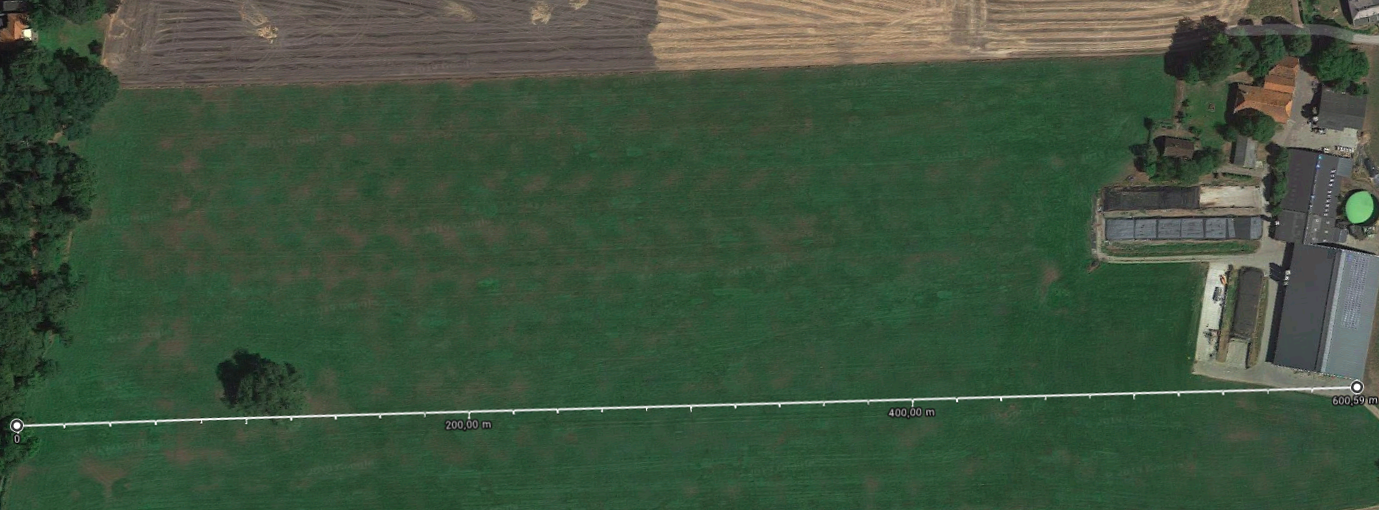
\includegraphics[width=.9\linewidth]{Afbeeldingen/meetmap.png}\end{center}
	\caption{Gebied voor het testen van de nRF24l01+.}
	\label{fig:testgebied}
\end{figure}

Op de aanwezige boerderij wordt geen WiFi gebruikt en de wel aanwezige apparatuur, die op de \SI{2,4}{\giga\hertz} zit, is op vliegtuigstand gezet.

\begin{figure}[H]
	\begin{center}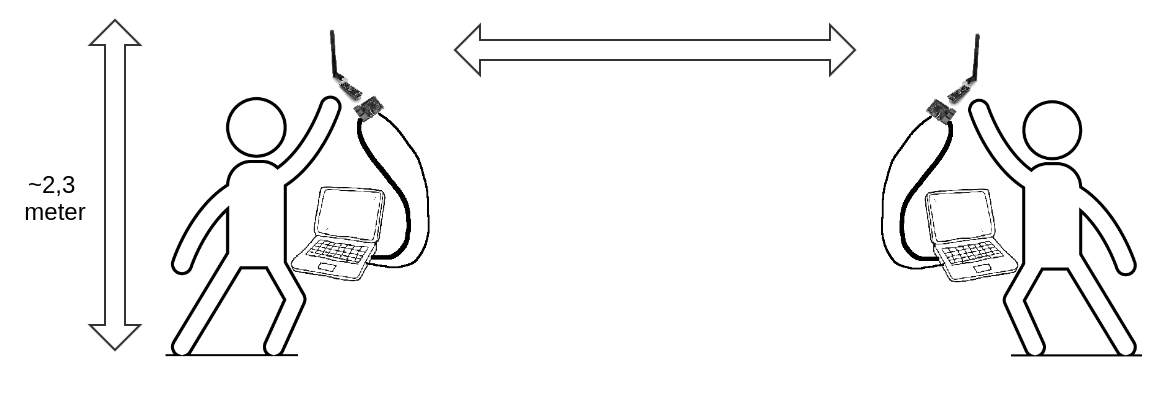
\includegraphics[width=.9\linewidth]{Afbeeldingen/comopstelling.png}\end{center}
	\caption{Testopstelling nRF24l01+ communicatie.}
	\label{fig:testopstelling}
\end{figure}


Het experiment wordt door de uitvoerende student en een medestudent uitgevoerd door op elke 50 meter een antenne hoog te houden om zo vrij zicht te creëren.


\begin{figure}[H]
	\begin{center}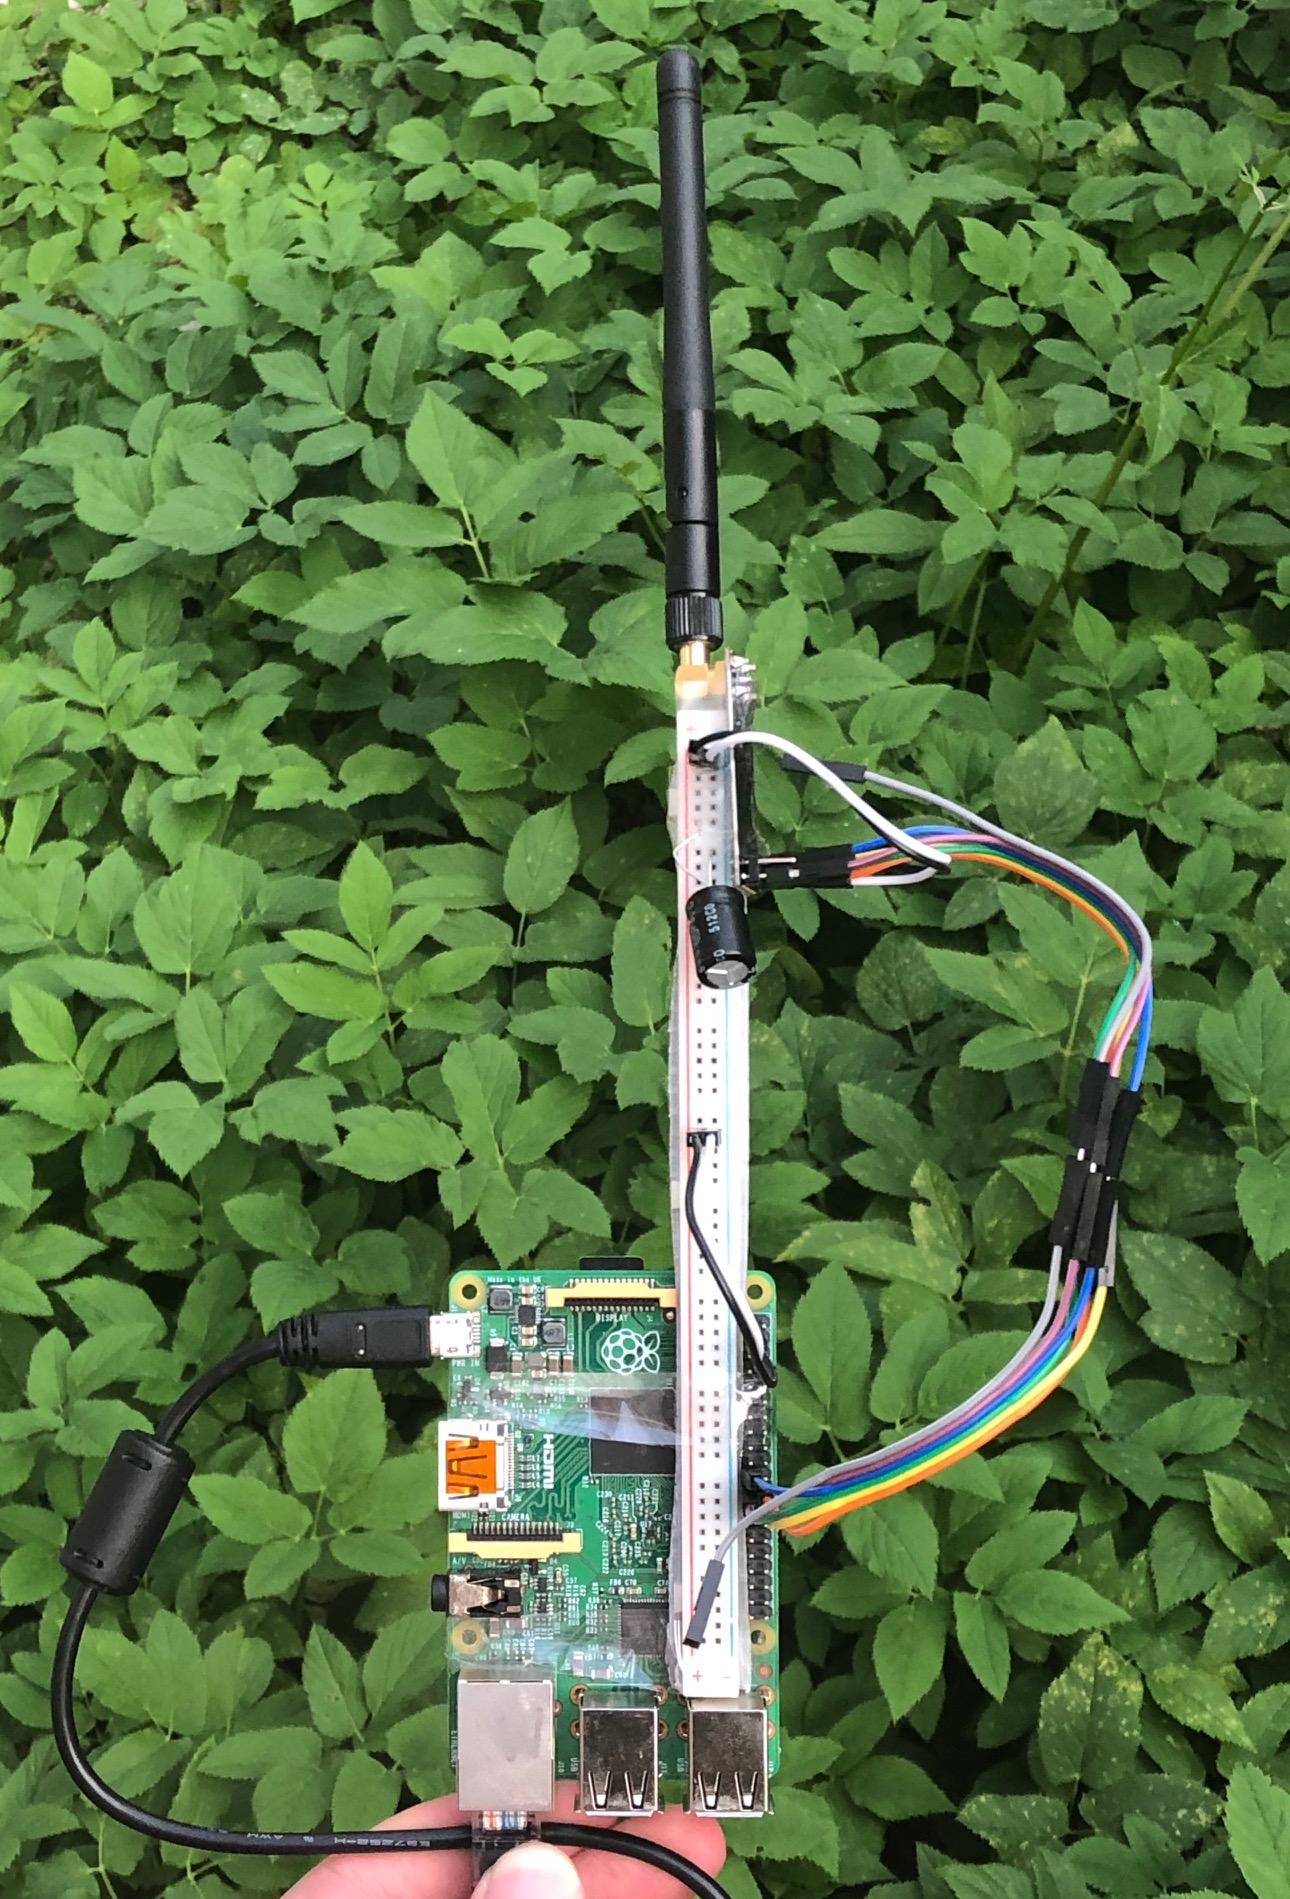
\includegraphics[width=.5\linewidth]{Afbeeldingen/testmodule.jpeg}\end{center}
	\caption{Netwerkmodule gebruikt in de test.}
	\label{fig:testmodule}
\end{figure}

Er is een test uitgevoerd waarbij er een netwerkmodule 1000 pakketten verstuurd naar de andere netwerkmodule die op zijn beurt weer een acknowledgement per pakket terug stuurt. De test is op elke 50 meter tot en met 600 meter afstand herhaald. Op elke punt is de test negen keer uitgevoerd. De resultaten zijn vervolgens opgeslagen in Microsoft Excel. 

\subsection{Resultaten}

In de bijlage \ref{app:testresultaten-lange-afstandtest-nrf24l01} zijn de exacte resultaten van de test terug te vinden.
Deze resultaten zijn verwerkt de grafiek te zien in \autoref{fig:grafiektestresultaten }

\begin{figure}[H]
	\begin{center}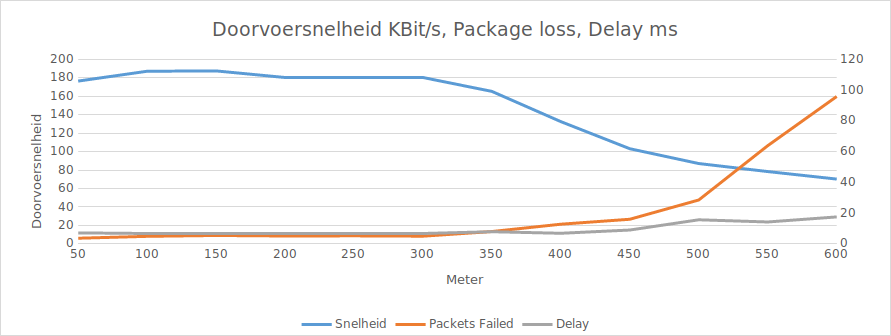
\includegraphics[width=1\linewidth]{Afbeeldingen/meetresultaten.png}\end{center}
	\caption{Grafiek gebaseerd op testresultaten NRF24l01+.}
	\label{fig:grafiektestresultaten }
\end{figure}

In de grafiek wordt zichtbaar dat de netwerkmodules altijd pakketten verliezen tijdens het zenden.
De eis die gesteld was is dat dit niet meer 5 procent mocht zijn op 500 meter.
Bij 500 meter verliest de module gemiddeld 28,55 van de 1000 pakketen waarbij de hoogste uitschieter 41 pakketten is.
Dit houdt in dat er dus gemiddeld 2,85 procent pakketten verloren gaan met een uitschieter van 4,1 procent.
Daarmee wordt de eis behaald van een maximum van 5 procent verlies. 

Een interessante trend in de grafiek is dat hoewel de snelheid vanaf 300 meter afneemt, de delay pas toeneemt bij 500 meter. 
Er is onvoldoende onderzoek aanwezig om te onderbouwen waarom dit is.
Een hypothese is dat de boom die niet direct in het zicht staat maar wel aanwezig is na 500 meter invloed heeft op het signaal. 
Dit omdat het signaal die tegen de boom aankomt ook terug zal reflecteren waardoor het kan storen.  


\chapter{Conclusie}
\label{chapter:conclusie}
In dit hoofdstuk wordt een conclusie getrokken op de vraag: Hoe kunnen een netwerkmodules een groep van ongeveer honderd drones voorzien van een onderling meshnetwerk die snel reageert op uitval van netwerkpunten?

Dit wordt vervolgt met een advies die voortvloeit uit de kennis van dit verslag.

\section{Antwoord op de hoofdvraag}

Uit de resultaten van dit onderzoek is gebleken dat door het combineren van een drone met een controller die zelfstandig kan opereren, een meshnetwerk opgezet kan worden van honderd drones. De controller moet toegang hebben tot een antenne voor onderlinge communicatie waarbij het advies is om gebruik te maken van een \nameref{sec:nrf24l01} vanwege zijn bereik en snelheid. Het onderzoek heeft de fase bereikt waarin de nRF24l01+ module aangesloten op een Raspberry Pi met de ontwikkelde software getest is maar nog wel in de kinderschoenen staat. 

Om het netwerk te kunnen opbouwen en onderhouden wordt een aangepaste variant van de reactieve routeringstechniek LMR toegepast. Belangrijk bij het gebruiken van deze techniek is dat de individuele netwerkpunten in staat zijn te kunnen verifiëren dat er een verbinding bestaat. De routeringstechniek is aangepast zodat deze zich enigszins proactief gedraagt door het versturen van heartbeats naar de gateway waarmee routes onderhouden worden. 

\section{Advies}
Het advies uit dit onderzoek luidt als volgt:

Op het moment dat Alten besluit om drones in te gaan zetten voor het verspreiden van netwerken zal zij zich bewust moeten zijn van haar plan voor dit netwerk.
Het aangepaste LMR protocol is geschikt voor een netwerk waarbij de drones zich verspreiden over een gebied en zich incidenteel verplaatsen naar een ander punt.
Dit is zo gemaakt omdat dit zo aangegeven is door Alten.
Op het moment dat Alten besluit dat de drones een andere gedrag krijgen zoals swarming dan is het protocol ongeschikt en is het advies om te kijken naar een reactief protocol die altijd nieuwe paden berekend.
Als Alten besluit dat de drones altijd op een zelfde positie zullen staan, dan zal een proactief protocol een beter alternatief zijn om zo berichten over het kortste pad te kunnen sturen.    

Dit onderzoek heeft daarnaast aangetoond dat de simulatiesoftware gebruikt kan worden voor het testen van geautomatiseerde herverdelingen bij uitval van netwerkpunten. 
Het advies is wel om het huidig geïmplementeerde herstelprotocol niet te gebruiken, aangezien deze te veel negatieve kenmerken heeft. 

\bibliographystyle{apacite}
\bibliography{bilbliography.bib}

\clearpage
\appendix
\chapter{Schets voor casus drone netwerk}
 \label{app:schetsNetwerk}
\begin{figure}[H]
	\begin{center}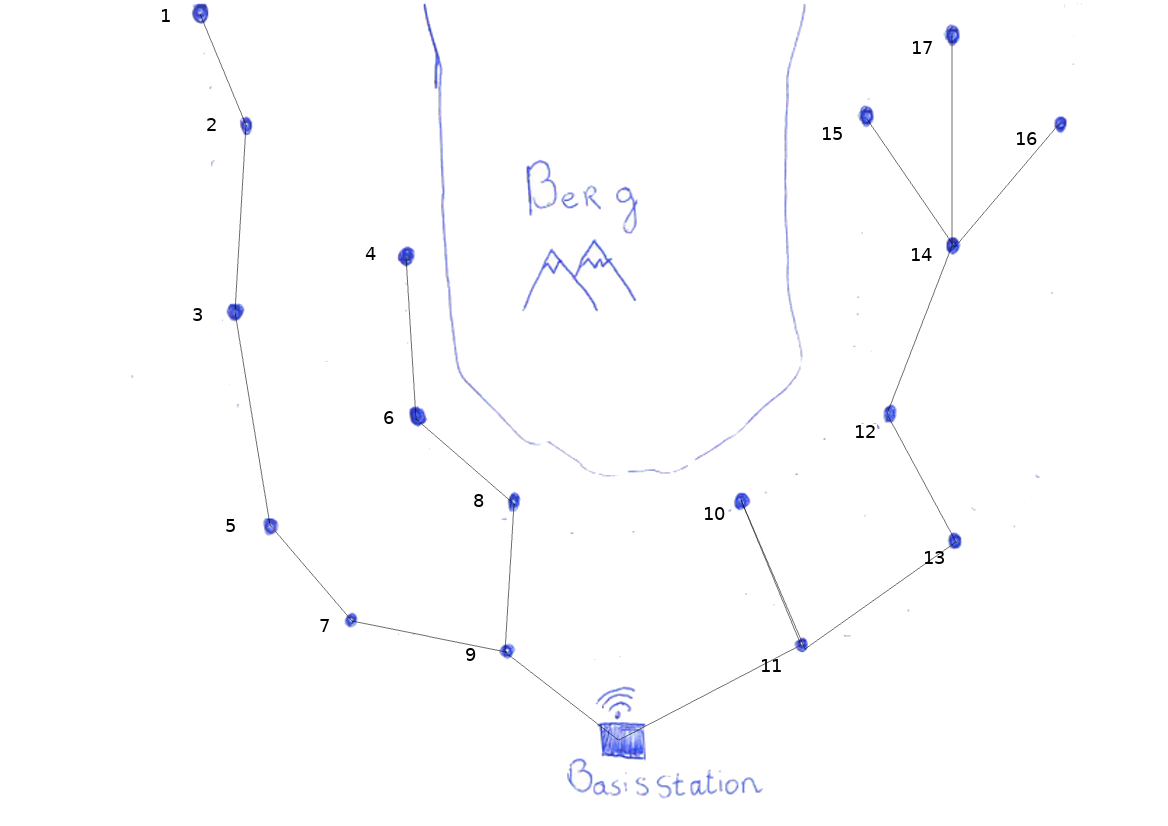
\includegraphics[width=\linewidth]{schetsNetwerk}\end{center}
	\caption{Schets van casus netwerk.}
	\label{fig:schetsNetwerk}
\end{figure}

\chapter{Testresultaten lange afstandtest nRF24l01+}\label{app:testresultaten-lange-afstandtest-nrf24l01}
\begin{center}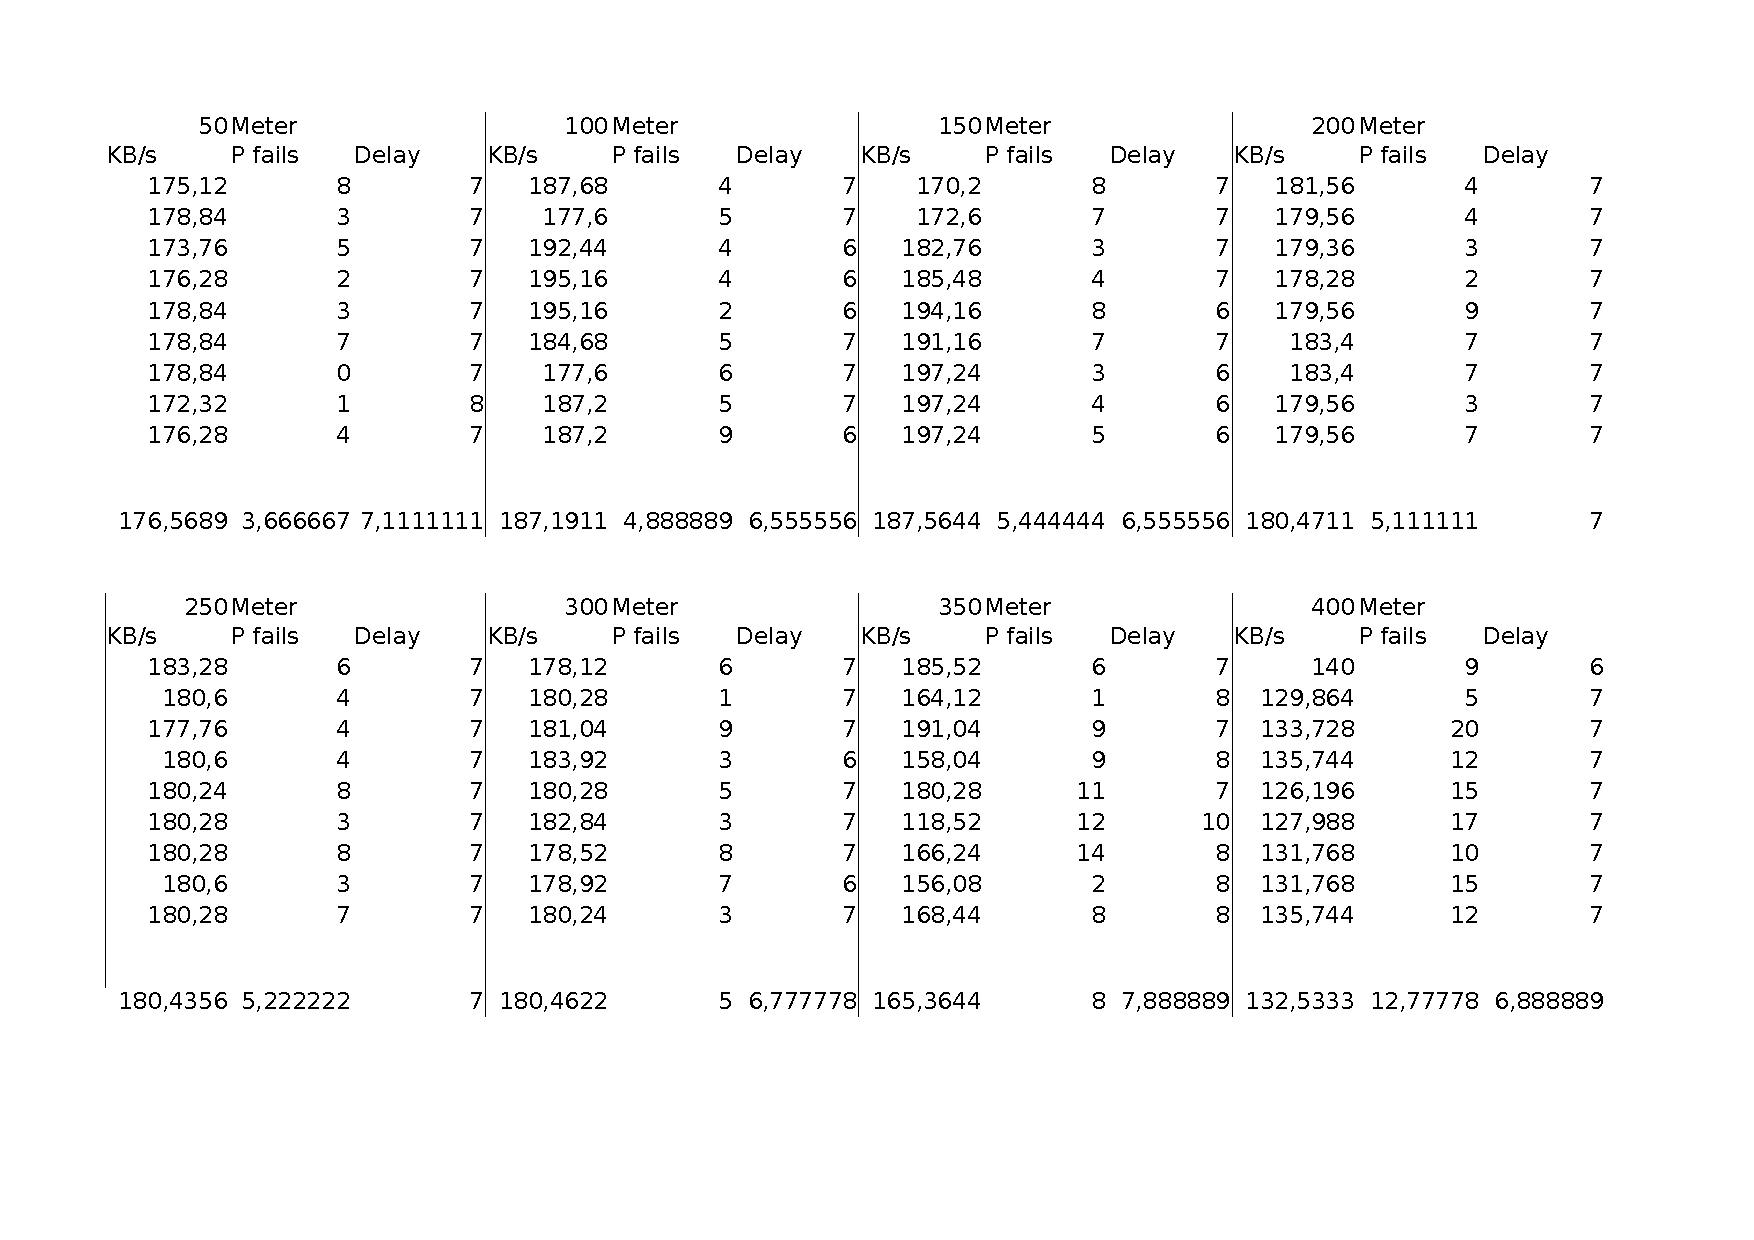
\includegraphics[page=1,width=.8\linewidth]{Bijlagen/Meetresultatennrflongrange.pdf}\end{center}
\begin{center}\includegraphics[page=2,width=.8\linewidth]{Bijlagen/Meetresultatennrflongrange.pdf}\end{center}
./Bijlagen/Meetresultatennrflongrange.pdf

\chapter{Videos simulatie netwerkherstel door drone verplaatsing}\label{sec:videos-simulatie-netwerkherstel-door-drone-verplaatsing}
De video's van deze bijlagen zijn te vinden door het volgende pad te volgen: \newline
./Bijlagen/Videos simulatie netwerkherstel door drone verplaatsing/
\section{enkele verloren drone situatie 1.mp4}\label{sec:enkele-verloren-drone-situatie-1mp4} Video van een enkele drone die verbinding verliest en dit met een enkele stap weer opbouwt.
\section{enkele verloren drone situatie 2.mp4}\label{sec:enkele-verloren-drone-situatie-2mp4} Video van een enkele drone die verbinding verliest en nadat een enkele stap niet werkt weer terugkeert naar de gateway.
\section{groep verloren drones situatie 1.mp4}\label{sec:groep-verloren-drones-situatie-1mp4} Video van een groep verloren drones waarbij het terugzetten van een enkele stap van een drone verbinding weer herstelt.
\section{groep verloren drones situatie 2.mp4}\label{sec:groep-verloren-drones-situatie-2mp4} Video van een groep verloren drones waarbij twee drones een verplaatsing moeten uitvoeren voor het herstellen van het netwerk.
\section{groep verloren drones situatie 3.mp4}\label{sec:groep-verloren-drones-situatie-3mp4} Video waarbij alle werkende drones terug keren naar de gateway omdat er geen herstel wordt gevonden.




\end{document}